\documentclass[twoside, xetex]{report}
%report中的chapter仅仅在新页开始,不强制在奇数页。
\usepackage{hcypaperstyle}

\begin{document}

\title{{\Huge 本科毕业设计论文\\}基于动态链接技术的web服务器动态扩展功能接口的设计与实现}
\author{黄丛宇\\06161032\\指导老师:马瑞芳}
\date{\today}

%\maketitle
\lfour

\zhabstract 

Web服务器作为互联网的核心组成部分,在支撑整个互联网服务中,起到了至关重要的作用。由于互联网中应用的不断更新,要求web服务器也能适应这种更新变化。同时,web服务器必须保证7*24小时的运行。在目前的正在使用的web服务器中,大部分都不支持功能的动态增加,也就是在不重启服务器的情况下,动态的为服务器增加功能。

本论文的主要内容是研究实现基于动态链接技术的Web服务器动态加载功能的接口。首先,介绍本课题的背景和意义以及作者的主要任务和工作,概述与本课题相关的HTTP协议(RFC2616)的内容,简单介绍动态链接技术及其使用,介绍Web服务器的一些主流设计和实现方法。然后,通过对HTTP协议的分析,设计插件的接口,分析动态链接技术,设计动态加载插件的过程。然后,采用非阻塞I/O+线程池+I/O多路复用技术,设计服务器的架构。本系统实现了服务器的基本功能,重点实现模块动态加载特性,并对实现进行测试。

最后,通过测试和观察运行结果,分析服务器是否可以正确处理HTTP请求,包括HTTP/1.1的持久连接和HTTP/1.0的非持久连接,并返回客户端所请求的资源。同时,验证插件接口的设计能否满足扩展功能的需求,能否正确的动态加载插件。

{\zhkeywords Web服务器;接口;Linux;C;动态加载}

\enabstract
	As the core component of the Word Wide Web, the web sever acts as a very important role to support the whole internet service. Due to the continuous update of the internet application, the web server must adapt this update. At the same time, the web server must keep running 7 * 24 hours. In the web servers which are used now, all most of them do not support to dynamically adding functions. Namely, when the server is running and dose not reboot, we can add new function to the server. 
	
	The main content of this paper is that studying the interface of dynamically loading function of the web sever based on dynamic link technology. First, the paper introduces the background and significance of this issue and the main task and job of the author. Then, the paper outlines the HTTP protocol(RFC 2616) and the dynamic link technology and its application, also outlines some design and implement methods of the web server. Next, by analysising the HTTP protocol and the dynamic link technology, we design the interface of the plugin and the process of dynamically loading the function plugin. Then, using nonblocking I/O, thread pool and I/O multiplexing, we design the architecture of the web server. This system implements the base functions of the web server and focuses on the implementation of the feature of dynamically loading function and testing the implementation.
	
	Last, by testing and the obsvervation of the run result, we analysis whether the server handle the HTTP request correctly and response to the client correctly or not, including HTTP/1.1 persistent connections and HTTP/1.0 nonpersistent connections. At the some time, we test whether the interface can santisfy the requirement of dynamically extending and dynamically load the function plugin correctly or not. 


{\enkeywords Web Server;Interface;Linux;C;Dynamically loading}
\setcounter{page}{1}
\tableofcontents

\chapter{绪论}
\setcounter{page}{1}

\section{背景和意义}
\subsection{Web服务器的背景}
	Web服务器也称为WWW(Word Wide Web)服务器,主要功能是提供网上信息浏览服务。Web服务器通过解析处理HTTP协议完成客户端的请求。当Web服务器接收到一个HTTP请求时,通过解析请求的内容,经过一些列的处理(如,查找客户端请求的资源),生成一个HTTP响应并发送给客户端。这个HTTP响应包含客户端所请求的数据(例如送回一个HTML页面)或者提示信息等。在处理一个请求,Web服务器可以返回给客户端一个静态页面或图片,进行页面跳转,或者把动态响应委托给一些其它的程序处理(例如CGI脚本,JSP脚本,ASP脚本,或者一些其它的服务器端技术)。这些处理委托请求的服务器端程序通常产生一个HTML的响应,并通过web服务器发送给客户端。
	
	目前,主流的web服务器包括Apache,Lighttpd和Nginx。
	\begin{itemize}
		\item Apache是世界排名第一的web服务器,是Apache软件基金会的一个开放源码的web服务器。Apache可以运行在几乎所有的计算机平台上,如,Linux,Windows,Unix等。Apache快速、可靠并且可通过简单的API扩充。
		\item Lighttpd是一个德国人领导的开源软件,根本在于提供一个专门针对高性能网站,安全、快速、兼容性好并且灵活的web服务器。Lighttpd具有非常低的内存开销,cpu占用率低,较好的性能以及丰富的模块。Lighttpd主要针对Unix/Linux平台,通过Cygwin也可以运行在Windows平台上,具有较好的夸平台特性。
		\item Nignx("engine x")是一个高性能的HTTP和反向代理服务器,也是一个IMAP/POP3/SMTP代理服务器。 Nginx是由Igor Sysoev为俄罗斯访问量第二的Rambler.ru站点开发的,它已经在该站点运行超过两年半了。Igor将源代码以类BSD 许可证的形式发布。尽管还是测试版,但是Nginx已经因为它的稳定性、丰富的功能集、示例配置文件和低系统资源的消耗而闻名了。
	\end{itemize}
	
	在这三个主流服务器的当前版本中,对于新的功能模块,都必须重启服务器才能是模块生效。然而有些时候,在怎加服务器功能的时候,不能对服务器进行重启,否则将会造成客户端当前状态的丢失,致使客户端当前正在进行的所有操作都将变的无效。比如,服务器和客户端保持了一个持久的连接,服务器不断的处理来自客户端的请求,而每个请求之间又保持着某种数据上的联系。也就是,前一个请求的处理结果影响下一个请求的处理结果。这时候,如果需要增加服务器的功能,同时增加的功能要立刻应用到当前的连接中,那么,服务器就不能进行重启。一旦服务器进行重启,由于HTTP协议不记录连接的状态,当前连接的所有状态都将丢失,那么,客户端的所有请求都将作废并重新开始。在一些场合,这将造成很严重的后果。
	
\subsection{动态链接技术背景}
	%程序员的自我休养---链接、装载和库 俞甲子 石凡 藩爱民 著 电子工业出版社
	动态链接技术是指,在程序的链接阶段,不对一些目标文件进行链接,等到程序运行时,再对这些目标文件进行链接的技术。也就是说,对于一些目标文件,把链接的过程推迟到了运行时在进行\ucite{cxyzwxy}。
	
	动态链接相对于静态链接有很多优点。对于静态链接,存在很严重的内存和磁盘空间的浪费,模块的更新也很困难。对于多个使用同一个库的程序,如果使用静态链接,那么每个程序的目标文件中都保存有这个库的一个副本。在程序运行的时候,每个程序在内存中也都有一个这个库的副本,这就对内存造成了很大的浪费。比如\ucite{cxyzwxy},在Linux系统中,一个普通的程序会使用到的C语言静态库至少在1MB以上,那么,如果在机器中有100个这样的程序,就要浪费掉近100MB的内存。如果磁盘中有2000个这样的程序,就要浪费近2GB的磁盘空间,很多Linux系统中,\verb|/usr/bin|下就有数千个可执行程序。另外,由于库是直接链接到程序的目标文件中的,一旦对库进行更新,将不会影响到程序中的副本,除非对程序进行重新编译。如果要对系统中所有使用这个库的程序进行重新编译,将是一个非常巨大的工作,很多情况下是不可能完成的(比如,没有程序的源文件)。比如,更新了Linux系统中的C语言静态库,那么就要对\verb|/usr/bin|下的那数千的程序进行重新链接。这将是一个繁重的工作。如果更新的是Windows系统中的库,由于很多程序无法获得源代码,也就无法进行重新链接,那么也就无法进行更新。
	
	动态链接则可以很好的解决上面的两个问题。当库是以动态链接的方式链接到程序中时,程序的目标文件中不包含有库的副本,仅仅是在调用库的地方做一个标记,同时在目标文件中记录所依赖的动态库。在程序运行时,操作系统从程序的目标文件中获知程序所依赖的动态库,然后在系统中查找这些动态库。接着,判断这些库是否已经加载到内存中,如果加载了,怎不需要在加载库,否则将库加载到内存中。如果有另一个程序需要同样的动态库,则不需要在将库加载到内存中,可以共享的使用内存中的副本。此时无论系统中运行了多少程序,所有的共享库在内存中只有一个副本,这就大大的提高了内存的使用效率。当需要对库进行升级的时候,仅仅需要将旧的库文件用新的覆盖掉,然后,重启系统中所有使用这个库的程序,那么所有程序都将使用新版的库。这就避免了对程序进行重新的链接。程序重启之后,库的更新工作急完成了。
	
	由于动态链接技术的这些特点,使得动态链接还具有另外一个特点:在程序运行时可以动态地选择加载各种程序模块。这个优点就可以用来制作程序的插件(Plug-in)。
	
\subsection{意义}
	在目前的正在使用的web服务器中,大部分都不支持功能的动态增加,也就是在不重启服务器的情况下,动态的为服务器增加功能。对于一些大型的应用,往往需要同时运行几百甚至几千台服务器,如果每增加一个功能都对服务器进行重启,将会浪费大量的时间,这就会造成很大的经济损失。而且,有些应用不允许服务器进行重启。比如,正在进行电子交易的系统,如果在某一时刻突然重启了服务器,可能造成这一时刻正在处理的交易中断,致使数据丢失。一旦数据发生了丢失,将是一件很严重的事故,会造成无法弥补的损失。
	
	针对这一问题,本课题基于动态链接库技术,使服务器在运行期间,可以动态的获知模块的增加并加载模块。当服务器可以动态的加载功能的时候,服务器可以在任何时间增加或者删除任意的功能。这样,服务器就避免了进行重启,也就可以有效的避免服务器重启带来的损失。
	
\section{课题目标及作者的主要工作}
	\subsection{课题目标}
	本课题通过分析HTTP协议(RFC2616),设计功能插件所需的接口。同时,对每一个接口定义其调用的时机和地点。通过使用动态链接技术,设计插件的动态加载的过程。最后,通过使用非阻塞I/O,I/O多路复用以及线程池的技术,构造出一个简单的Web服务器,并在这个服务器上实现所设计的接口以及接口的调用过程和加载过程。最终,通过这个简单的服务器,测试所设计的接口是否可用,功能能够动态的进行加载,服务器是否可以完成基本的HTTP协议解析和处理,正确的加载和调用插件。
	
	\subsection{作者主要工作}
	为了完成课题目标,本人主要需要完成如下具体工作:
	\begin{enumerate}
		\item 学习动态链接库和web服务器设计实现的相关知识和技术,包括I/O多路复用,HTTP协议等内容。                                
		\item 技术可行性论证,分析在使用动态链接技术的情况下,服务器能否完成动态加载功能的任务以。需求分析,分析系统所包含的主要功能。构造系统结构,完成系统框架的构造。
		\item 搭建开发环境,包括linux,gcc,gdb等。编码实现所有关键功能,包括HTTP协议的解析,处理HTTP请求,功能插件的加载和调用。 
		\item 测试插接接口的额可用性,分析系统是否达到了课题的目标。
		\item 撰写毕业设计论文,翻译外文资料。     
	\end{enumerate}
	
\section{论文章节结构}
	\subsection*{第一章是绪论,主要对本论文的主要内容进行了概述。}
	
	首先介绍了Web服务器和动态链接技术的背景。列举出当前主流的Web服务器的主要特定。在加载模块时都要对服务器进行重启。下面是课题的主要目标和作者的主要工作。最后,给出了本文的章节安排。
	
	\subsection*{第二章介绍了相关协议和技术,主要介绍HTTP协议和当前主流的服务器的设计和实现技术}
		首先介绍了动态链接技术在主流平台上的实现,以及动态库的创建和使用。接下来介绍了有关非阻塞I/O和I/O多路复用的特点。下面介绍了线程池的设计和使用,以及线程池的优点。最后,介绍了状态机的一些基本知识。
		
	\subsection*{第三章是动态扩展功能接口和服务器的分析和设计。包括分析RFC2616,根据HTTP协议设计接口,使用主流技术设计服务器。}
		首先是对HTTP协议(RFC2616)进行分析,设计插件的接口以及接口在处理HTTP协议时调用的过程。基于动态链接技术,设计模块的动态加载的过程,并给出设计方案。然后,介绍了服务器的I/O设计。
	
	\subsection*{第四章是动态扩展功能接口和服务器的实现和测试。主要是在Linux平台下实现插件接口和服务器,并对其进行测试}
		首先是插件接口的实现,通过使用C语言的结构体,将每个插件与一个结构体对应,来实现对插件的管理和调用,。接着是介绍动态加载过程的实现,实现动态加载。然后,实现插件在处理HTTP协议时的调用过程。下面是服务器的I/O实现。最后,通过对系统的测试。
		
	\subsection*{第五章为总结和展望。包括整篇论文的总结和对Web服务器设计的未来的展望}
		首先总结了本人在整个毕业设计期间的工作以及经验和教训。
		
		然后是展望,对Web服务器领域的前景做出展望,提出课题中所设计的服务器的不足和改进。
	
\chapter{Web服务器相关协议和技术}

\section{HTTP协议}
	HTTP协议(Hypertext Transfer Protocol,超文本传输协议)是一个属于应用层的面向对象的协议。它于1990年提出。主要用于从WWW服务器传输超文本到本地浏览器的传送协议。
	
	HTTP是一个客户端和服务器端请求和应答的标准。客户端是终端用户,服务器端是网站。通过使用Web浏览器、网络爬虫或者其它的工具,客户端发起一个到服务器上指定端口(默认端口为80)的HTTP请求。应答的服务器上存储着(一些)资源,比如HTML文件和图像。我们称这个应答服务器为源服务器(origin server)。
	
	通常,由HTTP客户端发起一个请求,建立一个到服务器指定端口(默认是80端口)的TCP连接。HTTP服务器则在那个端口监听客户端发送过来的请求。一旦收到请求,服务器(向客户端)发回一个状态行,比如"HTTP/1.1 200 OK",和(响应的)消息,消息的消息体可能是请求的文件、错误消息、或者其它一些信息。通过HTTP或者HTTPS协议请求的资源由统一资源标识符(Uniform Resource Identifiers,URI)来标识。
	
	HTTP/1.1协议中共定义了八种方法(有时也叫“动作”)来表明Request-URI指定的资源的不同操作方式:
	\begin{enumerate}
		\item OPTIONS 返回服务器针对特定资源所支持的HTTP请求方法。也可以利用向Web 服务器发送'*'的请求来测试服务器的功能性。
		\item HEAD 向服务器索要与GET请求相一致的响应,只不过响应体将不会被返回。这一方法可以在不必传输整个响应内容的情况下,
					就可以获取包含在响应消息头中的元信息。
		\item GET 向特定的资源发出请求。注意:GET方法不应当被用于产生“副作用”的操作中,例如在Web Application中。
					其中一个原因是GET可能会被网络蜘蛛等随意访问。参见安全方法
		\item POST 向指定资源提交数据进行处理请求(例如提交表单或者上传文件)。数据被包含在请求体中。POST请求可能会导致新的资源的建立和/或已有资源的修改。
		\item PUT 向指定资源位置上传其最新内容。
		\item DELETE 请求服务器删除Request-URI所标识的资源。
		\item TRACE 回显服务器收到的请求,主要用于测试或诊断。
		\item CONNECT HTTP/1.1协议中预留给能够将连接改为管道方式的代理服务器。
	\end{enumerate}
	
	HTTP服务器至少应该实现GET和HEAD方法,其他方法都是可选的。当然,所有的方法支持的实现都应当符合下述的方法各自的语义定义。此外,除了上述方法,特定的HTTP服务器还能够扩展自定义的方法。
	
	所有HTTP响应的第一行都是状态行,依次是当前HTTP版本号,3位数字组成的状态代码,以及描述状态的短语,彼此由空格分隔。状态代码的第一个数字代表当前响应的类型:
	\begin{itemize}
		\item 1xx 消息——请求已被服务器接收,继续处理
		\item 2xx 成功——请求已成功被服务器接收、理解、并接受
		\item 3xx 重定向——需要后续操作才能完成这一请求
		\item 4xx 请求错误——请求含有词法错误或者无法被执行
		\item 5xx 服务器错误——服务器在处理某个正确请求时发生错误
	\end{itemize}
	%http://zh.wikipedia.org/zh-cn/%E8%B6%85%E6%96%87%E6%9C%AC%E4%BC%A0%E8%BE%93%E5%8D%8F%E8%AE%AE
\section{动态链接技术}
	\subsection{动态链接的实现}
	动态链接设计运行时的链接及多个文件的加载,必须要有操作系统的支持,因为动态链接的情况下,进程的虚拟地址空间的分部会比静态链接情况下更为复杂。目前主流的操组系统的几乎都支持动态链接这种方式,在Linux系统中,ELF动态链接文件被称为动态共享对像(DSO,Dynamic Shared Objects),简称共享对象,他们一般是以“.so”为扩展名的一些文件。在Window系统中,动态链接文件被称为动态链接库(DLL, Dynamicla Linking Library),它们通常是我们平时很常见的".dll"为扩展名的文件。
	
	在程序被加载时,系统的动态链接器会将程序所需要的所有动态链接库装载到进程的地址空间中,并且程序中所有未决议的符号绑定到响应的动态链接库中,并进行重定位工作。动态链接把链接这个过程从程序加载前推迟到程序加载时,这会造成程序性能上的一些损失。据估算,动态链接与静态链接相比,性能损失大约在5\%以下。
	
	\subsection{动态库的创建和使用}
	在Linux下和Window下,动态库的创建和使用是不相同的。由于本课题主要是在Linux系统中进行,因此在这里,将通过一个例子来简单的介绍在Linux下动态库的使用\ucite{cxyzwxy}。例子的程序源码如下:
	\begin{verbatim}
	/* Program1.c*/
	#include "Lib.h"
	int main(int argc, char *argv[])
	{
		foobar(1);
		return 0;
	}
	
	/*Program2.c*/
	#include "Lib.h"
	int main(int argc, char *argv[])
	{
		foobar(2);
		return 0;
	}
	
	/*Lib.c*/
	#include <stdio.h>
	void foobar(int i)
	{
		printf("Printing from Lib.so %d\n", i);
	}
	/*Lib.h*/
	#ifndef LIB_H
	#define LIB_H
	void foobar(int i);
	#endif
	\end{verbatim}
	程序很简单,两个程序的主要模块Program1.c和Program2.c分别调用Lib.c里面的foobar()函数。
	在Linux下,我们使用gcc讲Lib.c编译成一个共享库:
\begin{verbatim}
	gcc -fPIC -shared -o Lib.so Lib.c
\end{verbatim}
	-fPIC和-shared是GCC的参数,这也是创建共享库的关键参数:
	\begin{itemize}
		\item -fPIC 表示使用地址无关代码(Position Independent Code)技术来产生输出文件。
		\item -shared 表示输出结果是共享库类型。
	\end{itemize}
	
	这时候,我们得到了一个Lib.so文件,这就是包含了Lib.c的foobar()函数的共享对象文件。然后,我们分别编译链接Program1.c和Program2.c:
	\begin{verbatim}
	gcc -o Program1 Program1.c ./Lib.so
	gcc -o Program2 Program2.c ./Lib.so
	\end{verbatim}
	在链接程序Program1时,没有将动态库链接到程序的目标文件中,而仅仅是做了一个标记。当系统加载程序Program1时,动态链接加载器会根据Program1目标文件中的信息,搜索共享库Lib.so并加载到内存中。完成最后的链接工作。
	
\section{非阻塞I/O与I/O多路复用}
	非阻塞I/O使我们可以调用open、read和write这样的I/O操作,并使这些操作不会永远阻塞。如果这种操作不能完成,则调用立即出错返回,表示该操作如继续执行将阻塞。\ucite{apue}
	
	对于一个给定的描述符有两种方法对其置顶非阻塞I/O:
	\begin{enumerate}
		\item 如果调用open获得描述符,则可指定O\_NONBLOCK标志。
		\item 对于已经打开的描述符,则可调用fcntl,有该函数打开O\_NONBLOCK文件状态标志。
	\end{enumerate}
	
	I/O多路复用(或者I/O多路转接,I/O multiplexing),是指先构造一张有关描述符的列表,然后调用一个函数,知道这些描述符中的一个或多个已准备好进行I/O时,该函数返回,在返回时,它告诉进程那些描述符已经准备好进行I/O。\ucite{apue}
	
	I/O多路复用有多种实现。主要包括:
	\begin{enumerate}
		\item 传统的select 对所监听的描述符数量有一个硬性的限制:FD\_SETSIZE。这个限制通常很难改变。另外,随着所监听的描述符的数量的增加,select的效率有明显的下降。这是由于select要对所有被监听的描述符进行扫描。
		\item 传统的poll 对监听的描述符数量没有硬性的限制。真正的显示通常来自机器的内存大小等。和select一样, 随着描述符的增加效率明显降低。
		\item /dev/poll 是Solaris中poll的替代品。
		\item kqueue 是FreeBSD中的poll的替代品。(也是NetBSD的)
		\item epoll 在Linux 2.6内核中被引入。是epoll的替代品。对描述符的数量没有限制(限制通常来自内存大小),并且,效率不随描述符数量的增加而下降。
		\item Completion Port NT内核(Window平台)中I/O多路复用的实现。
	\end{enumerate}
	
	图\ref{epollvspoll}是有关epoll和poll的效率比较。sys\_epoll和/dev/epoll是epoll的不同接口。
	\begin{figure}[htbp]
	\centering
	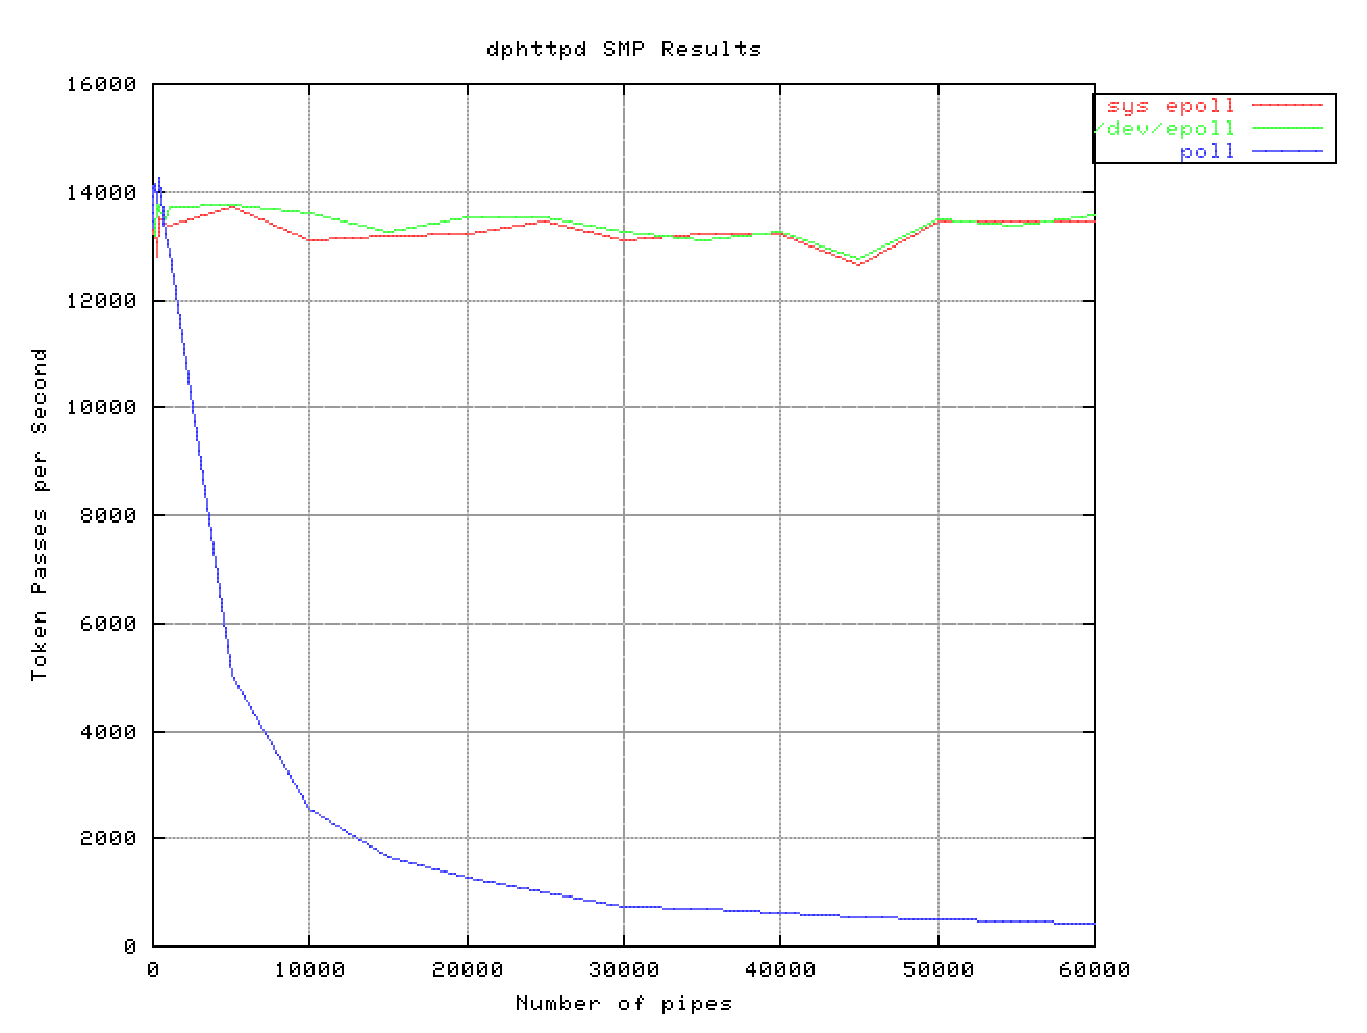
\includegraphics[height=11cm, width=15cm]{pics/epollvspoll.eps}
	\caption{epoll与poll效率比较}
	\label{epollvspoll}
	\end{figure}
	
	由于本课题主要是在Linux平台下进行,因此,系统中使用Linux下推荐的epoll。
	
	epoll主要有三个接口函数:epoll\_create, epoll\_wait, epoll\_ctl。
	\begin{enumerate}
		\item epoll\_create 创建一个epoll实例,并返回一个epoll的描述符。这个描述符是后面两个函数的参数。
		\item epoll\_wait 等待epoll实例所监听的描述符发生I/O事件。一旦有描述符发生事件,返回这些描述符和对应的事件。
		\item epoll\_ctl 增加或删除epoll实例所监听的描述符,或修改描述符所监听的事件。
	\end{enumerate}
	
	epoll有两种模式:水平触发(level-triggered)和边际触发(edge-triggered)。当在水平触发模式时,只要有描述符处于就绪状态(比如,有数据可读),那么调用epoll\_wait时,epoll\_wait立即返回描述符及其对应事件。而当处于边际触发时,当有描述符从不就绪变成就绪,epoll\_wait返回描述符及其事件,并且epoll假设调用这已经知道了事件的发生并且会进行正确的处理。之后,无论多少次调用epoll\_wait,只要描述符的状态不发生变化(从不就绪变成就绪),就算此时有数据可以读,epoll都不会再次提醒调用者。这就有可能造成数据丢失。
	epoll默认处在水平触发模式。
	
\section{线程池}
	虽然线程的创建和初始化相对于进程来说,已经很快速了。但是,在很多程序中,特别是负载较高的服务器程序,频繁的创建销毁线程也会影响程序的运行效率。而线程池则可以避免掉对线程的频繁的创建和销毁。
	
	在线程池中通常会有若干个处于等待状态的线程。这些线程仅仅是处于等待状态,各种资源都是已经分配好的。当需要线程来处理某一个任务时,通过线程池获得一个处于等待状态的线程,然后通知这个线程去处理这个任务。此时的线程可以立即执行任务(准确的说是立即处于就绪状态),而不需要花费时间进行初始化等工作。当处理完任务后,线程重新回到线程池中,继续处于等待状态,直到下次任务到达。
	
	线程池中关键的是如何通知处于等待状态的线程有新的任务需要处理。这需要对应平台的线程库予以支持。在Linux下,线程的使用通常依赖pthread库。pthread库提供了一套线程的创建管理方法。其中,条件变量可以很好的实现通知等待线程的功能。条件变量是指线程等待某一事件的发生,在事件发生之前,线程一直处于等待状态。

\section{状态机}
	状态机,即有限状态机(Finite State Machine)。是表示有限个状态以及在这些状态之间的转移和动作等行为的数学模型。
	
	图\ref{fsm}是一个简单的关于开门和关门的状态机。
	
	\begin{figure}[htbp]
	\centering
	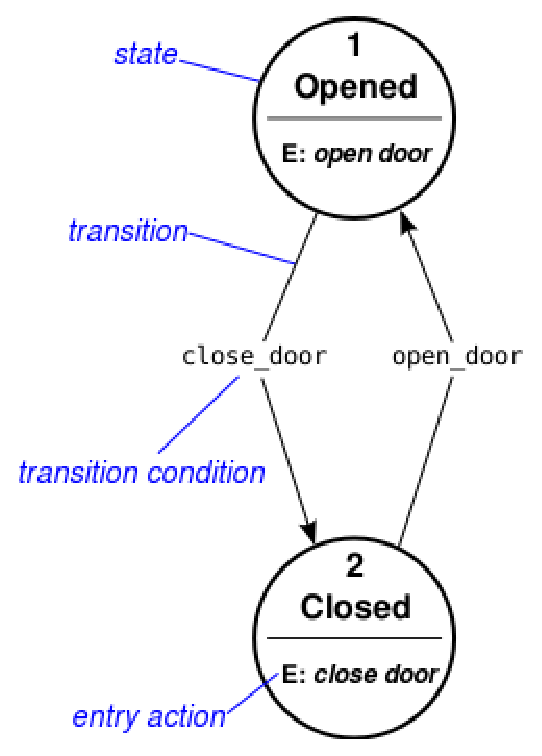
\includegraphics[height=8cm, width=6cm]{pics/fsm.eps}
	\caption{开门关门状态机}
	\label{fsm}
	\end{figure}
	
	状态机可分为确定型(DFA)和非确定型(NDFA、GNFA)状态机。在确定型状态机中,每个状态对每个可能输入只有精确的一个转移。在非确定型状态中,给定状态对给定可能输入可以没有或有多于一个转移。
	
\section{本章小结}
	在本章中,首先对HTTP协议进行了概述,包括HTTP协议的历史,主要的方法以及状态码等。接着概述了动态链接技术,包括动态链接技术在linux平台下的实现以及怎样创建和使用动态链接库。然后简单介绍了非阻塞I/O和I/O多路复用的相关内容,包括I/O多路复用的各种实现及其性能比较以及epoll的使用。最后简单的介绍了状态机,包括状态机的定义和表示方法。
	
\chapter{动态扩展功能接口与服务器的分析和设计}
	
	Web服务器的主要工作就是根据HTTP协议处理客户端的请求,因此,HTTP协议是Web服务器的核心。在对服务器的功能进行怎加时,必须能够和HTTP协议的处理无缝接合。因此在本章中,首先对HTTP协议处理过程和数据格式进行了分析。在分析的基础之上,设计接口的具体内容以及接口的调用过程。为了实现动态加载功能,服务器必须动态的感知插件的增加。本章针对这个问题进行分析并给出了设计方案。对于服务器的分析和设计,着重描述了I/O处理和连接处理两个部分。
	
\section{动态扩展功能接口的分析和设计}
\subsection{HTTP协议的分析}
	HTTP协议的主要数据格式包括Request格式和Response格式。
	
	Request是客户端发送个服务器的请求数据。包括服务器完成请求所需要的信息。HTTP协议规定Request的格式如下:
\begin{verbatim}
    ---------------------------------------
    | Methods |sp| URI |sp| Version |cr|lf|  -----> Request line
    ---------------------------------------
    | Header Field Name: |sp| Value |cr|lf|  -]
    ---------------------------------------   |
    |   ... (more headers)                |   |---> Header lines
    ---------------------------------------   |
    | Header Field Name: |sp| Value |cr|lf|  -]
    ---------------------------------------
    |cr|lf|                                  -----> a blank line
    ---------------------------------------
    |                                     |
    | Data...                             |  -----> Entity body
    |                                     |
    ---------------------------------------
      cr = \r ; lf = \n ; sp = blankspace
\end{verbatim}
 	从上面的格式可以看出,Request的格式非常简单,包括Request line,Header lines和 Entity body三个部分。Request line包含请求的方法,请求资源的URI以及客户端所使用的HTTP协议的版本。其中,对于所请求的资源的URI中的特殊字符(如汉字),客户端要对其进行编码。编码的格式为“\% HEX HEX”(具体参见RFC 2396)。Header lines包含一些“key:value”形式的键值信息,是客户端发送给服务器的有关自身信息或者链接处理方式等数据。这些键值信息的键在HTTP协议中有明确的规定,服务器一般不对这些键值信息的意义进行更改或扩充HTTP协议规定之外的键值信息。Entity body中包含客户端发送给服务器的数据。这些数据通常对服务器透明,也就是说服务器不需要关心这些数据的意义,只需要将这些数据传递给一些处理链接请求的委托程序(如,CGI脚本),由这些委托程序进行处理。在HTTP协议中,没有对Entity body中的数据的格式和意义做任何形式的规定或定义。
 	
 	Response的格式与Request格式类似。Response数据由服务器处理完请求之后,发送给客户端。Response格式如下:
\begin{verbatim}
-----------------------------------------------
|Version|sp|Status-Code|sp|Reason-Phrase|cr|lf| ---> Status line
-----------------------------------------------
| Header Field Name:   |sp|  Value      |cr|lf| -]
-----------------------------------------------  |
|  ... (more headers)                         |  |-> Header lines
-----------------------------------------------  |
| Header Field Name:   |sp|    Value    |cr|lf| -]
-----------------------------------------------
|cr|lf|                                        ---> a blank line
-----------------------------------------------
|                                             |
| Data...                                     |  ---> Entity body
|                                             |
-----------------------------------------------
 cr = \r ; lf = \n ; sp = blankspace
\end{verbatim}
 	Response格式和Resquest格式的主要区别在第一行的Status line。Status line包含HTTP 协议的版本,请求处理结果的状态码和结果原因描述。Response中Header lines中的键值对和Request中的键值对一样,都是由HTTP协议进行明确的规定。Entity body包含处理结果。
 	
	通常,在HTTP协议中,有客户端发起请求,服务器被动的接受请求。如图\ref{httpbaike}
	\begin{figure}[htbp]
	\centering
	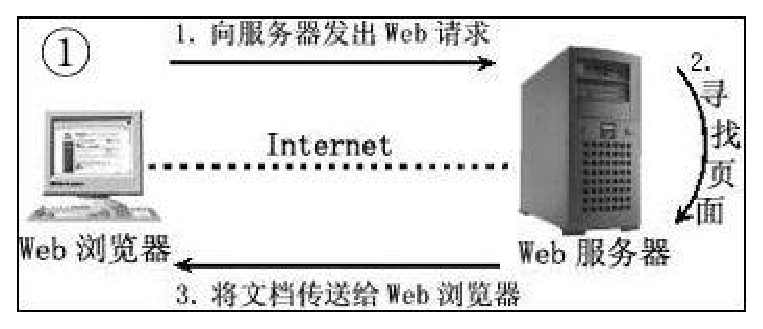
\includegraphics[height=3cm, width=8cm]{pics/httpbaike.eps}
	\caption{HTTP协议的处理过程}
	\label{httpbaike}
	\end{figure}
	
	在客户端和服务器之间建立连接之后,客户端发送Request数据,服务器对Request数据进行解析然后按照解析出来的数据对请求进行处理,处理完毕之后(包括处理出错),服务器构造Response数据,返回给客户端。在整个过程中,服务器对客户端的请求不做任何信息或者状态的记录。也就是说,即使是同一客户端的同一个请求,多次发送给服务器,服务器都认为是不同的请求。在本课题中,我们主要关心在服务器端HTTP协议的处理过程。如图\ref{serverhttp}。
	\begin{figure}[htbp]
	\centering
	\includegraphics[height=8cm, width=10cm]{pics/serverhttp.eps}
	\caption{服务器端HTTP协议的处理过程}
	\label{serverhttp}
	\end{figure}
	
\subsection{动态扩展功能接口调用过程的设计}
	在图\ref{serverhttp}中可以看到,服务器在处理HTTP请求的时候,基本上分为三步:解析协议,处理请求和返回处理结果。在解析协议和返回处理结果的过程中,服务器都要必须严格按照HTTP协议的规定进行处理,这两个过程中,没有必要也不能增加HTTP协议规定之外的处理步骤。并且,插件基本上都是针对处理请求设计的,因此,插件的调用过程集中在处理请求的阶段。插件的调用过程如图\ref{httpplugin}所示。
	\begin{figure}[htbp]
	\centering
	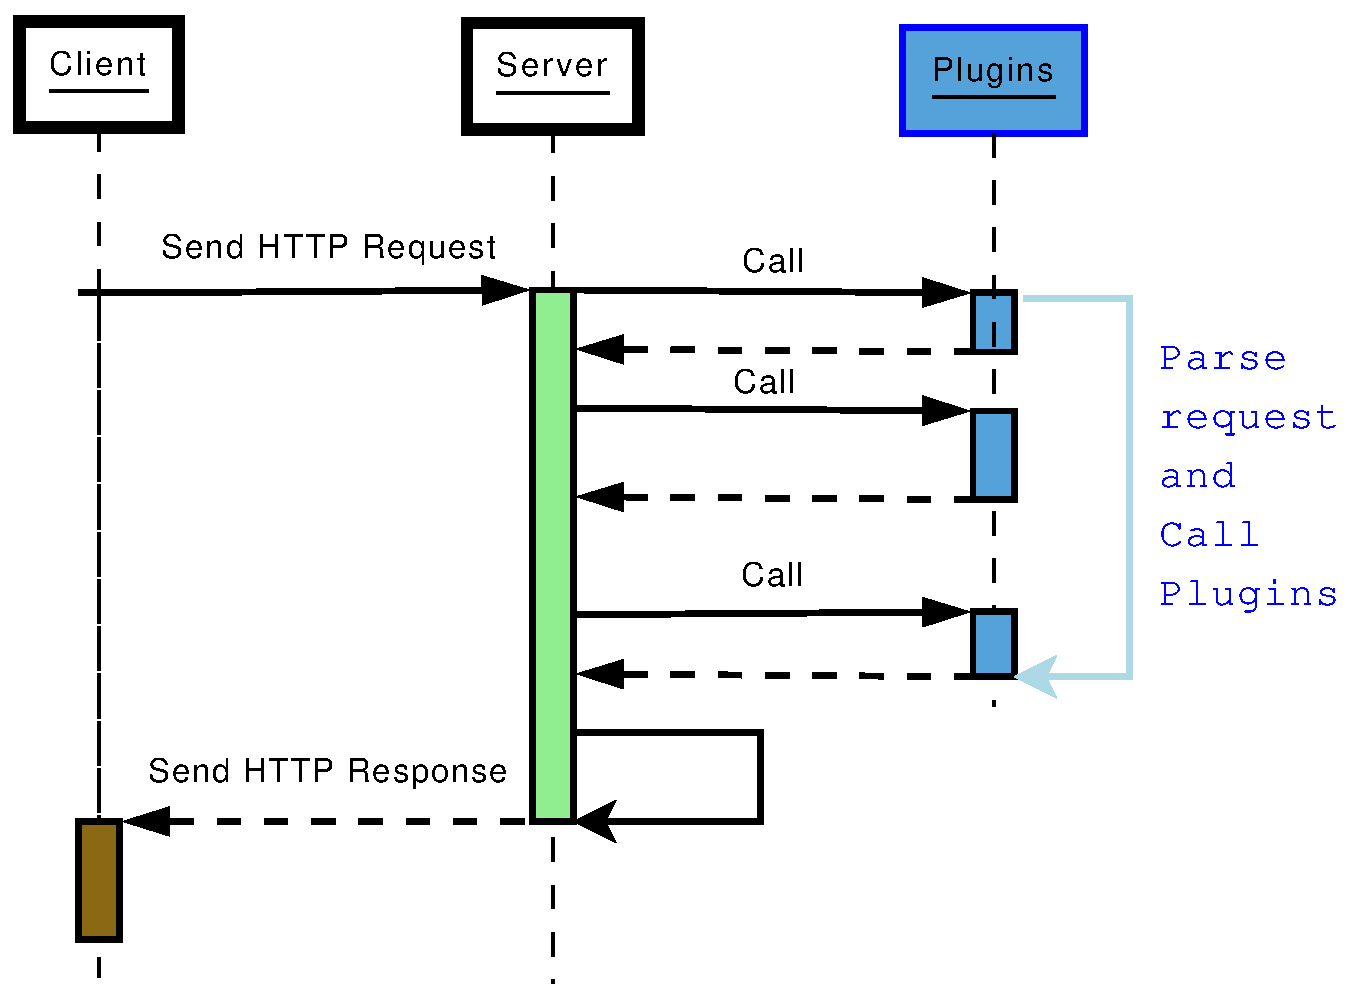
\includegraphics[height=9.5cm, width=12cm]{pics/httpplugin.eps}
	\caption{接口调用过程}
	\label{httpplugin}
	\end{figure}
	
	由于插件的具体功能对于服务器是透明的,服务器无法获知插件具体要对连接进行何种处理。服务器所知道的仅仅是插件所实现的接口。对于服务器而言,所有的插件都是一样的。当服务器处理某一个特定的请求时,服务器无法判断当前请求是否需要调用某一个插件进行处理。因此,服务器对于每一个请求,依次调用所有的插件。当某一个插件完成了对请求的处理之后,服务器将不在调用其他插件。服务器将这个插件的处理结果返回给客户端。那么,对于是否要对当前连接进行处理将有插件自己决定。比如,插件可以通过Request中的URI来判断是否需要对这个请求进行处理。
	
	由于插件的调用是按照一定的顺序进行的,因此,对于插件的调用就存在一个隐含的优先级。通常,最先加载的插件在处理请求的时候最先被调用。如果一个请求同时需要两个插件进行处理,那么,在第一个插件处理完毕之后,如果插件返回的是处理完毕,而不是继续处理,那么服务器将不会调用第二个插件进行处理。因此,通常情况下,插件处理完请求之后,应该告诉服务器继续调用其他插件处理请求,这样可以防止出现请求没有处理完毕的错误。
	
\subsection{动态扩展功能接口函数的设计}
	插件接口被定义一些列标准函数原型。所有函数都有明确的定义和调用时机。这些函数大部分都是在前一节中描述的处理请求的过程中被调用。还有一些函数则在其他一些地方调用,以完成一些辅助的任务。下面详细介绍这些接口。
	
	首先,需要定义插件的初始化等函数。这些函数不用来处理请求,而是做一些辅助性的工作,不是在服务器处理请求的过程中被调用。
	\begin{itemize}
		\item init: 初始化插件。只调用一次,在加载插件之后调用。
		\item set\_default: 设置插件的配置为默认值。只调用一次,在加载插件之后调用。
		\item cleanup: 清理插件。在卸载插件的时候只调用一次。
		\item trigger: 每秒钟调用一次。相当于计时器。可以用来完成一些周期性的任务。
		\item sighup: 处理挂断信号。在服务器接收到这个连接的挂断信号(SIGHUP)时调用。
		\item connection\_close: 连接关闭时调用。
		\item connection\_reset: 连接重置时调用。
		\item joblist: 在连接被加入到作业队列中调用。作业队列中的连接处在等待I/O事件的状态。
	\end{itemize}
	
	下面需要定义在处理请求时所要调用的函数。在前面分析HTTP协议数据格式和处理过程可以看出,Request中的URI用来对所请求的资源进行定位。对于不同的资源,可以调用不同的插件进行处理。比如,如果请求的资源是以".o"为扩展名,那么就可以通过这一扩展名来判断所请求的是一个CGI脚本,还是一个普通文件。通常,以".o"为扩展名的是一个CGI脚本,那么就可以调用CGI插件进行处理。
	
	处理请求的函数如下:
	\begin{itemize}
		\item url\_raw: 获得原始的URI后调用。也就是未对“\% HEX HEX”形式的字符进行解码的URI。
		\item url\_clean: 获得已解码的URI后调用。
		\item docroot: 设置插件工作的根目录 。在获得解码后的URI后调用。
		\item physical: 获得请求资源对应的物理地址后调用。
		\item subrequest\_start: 子请求开始。
		\item handle\_subrequest: 处理子请求。
		\item subrequest\_end: 子请求结束。
	\end{itemize}
	
	最后三个处理子请求的函数在服务器处理请求的最后阶段分别调用。
	
	这些函数仅仅规定了其调用的时间,对于其具体的任务不做任何限定。比如,插件可以在调用physical接口函数的时候,查找所请求的资源,也可以在调用subrequest\_end时进行查找。同时,将接口细分之后,插件可以只对请求做部分的处理。例如,插件统计某一资源的请求次数时,可以在调用physical函数的时候完成,而不需要等到请求处理完毕。这样可以给予插件以较高的灵活性。
	
	对于每一个插件,这些接口函数都是选择性的进行实现。服务器会对插件所实现的接口函数进行记录。对于没有实现的接口函数,服务器将不会调用。
	
	由于插件接口有可能会因为需求的改变而随着服务器的不断升级而发生改变。对于一些使用旧版本的插件,很有可能在新版本的服务器中无法使用。因此,必须对插件的版本进行控制。
	
	插件的版本控制采用如下方法:插件版本号分为两个部分:主版本号和次版本号,两个版本号依次排列,并用'.'分割。比如:2.3,主版本号为2,次版本号为2。服务器的主次版本号和插件接口的主次版本号必须一致。主版本号改变通常由于插件接口发生了变化,不同主版本号的插件和服务器不兼容。次版本号改变通常是由于对插件的接口进行了增加,同时兼容较低次版本号的版本。次版本号底的插件同样可以运行在次版本号高的服务器上,当然,前提是主版本号相同。但是,不保证次版本号高的插件可以运行在次版本号底的服务器上。通常,服务器还有第三个版本号——BUG修正版本号,这个版本号不会对插件接口产生影响,仅仅是服务器的BUG修正。因此,不需要考虑到插件设计中。
	
\subsection{动态加载过程的设计}
	为了进行动态的加载插件,服务器必须能实时的获知插件的增加。
	
	服务器可以通过检测插件的动态库所在的目录的变化,来获知是否有新的插件加入。但是,插件的动态库可能会放在不同的地方,这样就需要同时监测多个目录。这会影响服务器的效率。而且,一旦需要增加插件动态库存放的地方,必须通知服务器新增加的地方。这会增加服务器的复杂度。为了降低服务器的复杂度,本系统采用监测插件配置文件的方法。一旦插件配置发生更改(如,修改,删除等),服务器就重新读取插件配置文件,重新加载插件。监测的过程如图\ref{loadplugin}。
	\begin{figure}[htbp]
	\centering
	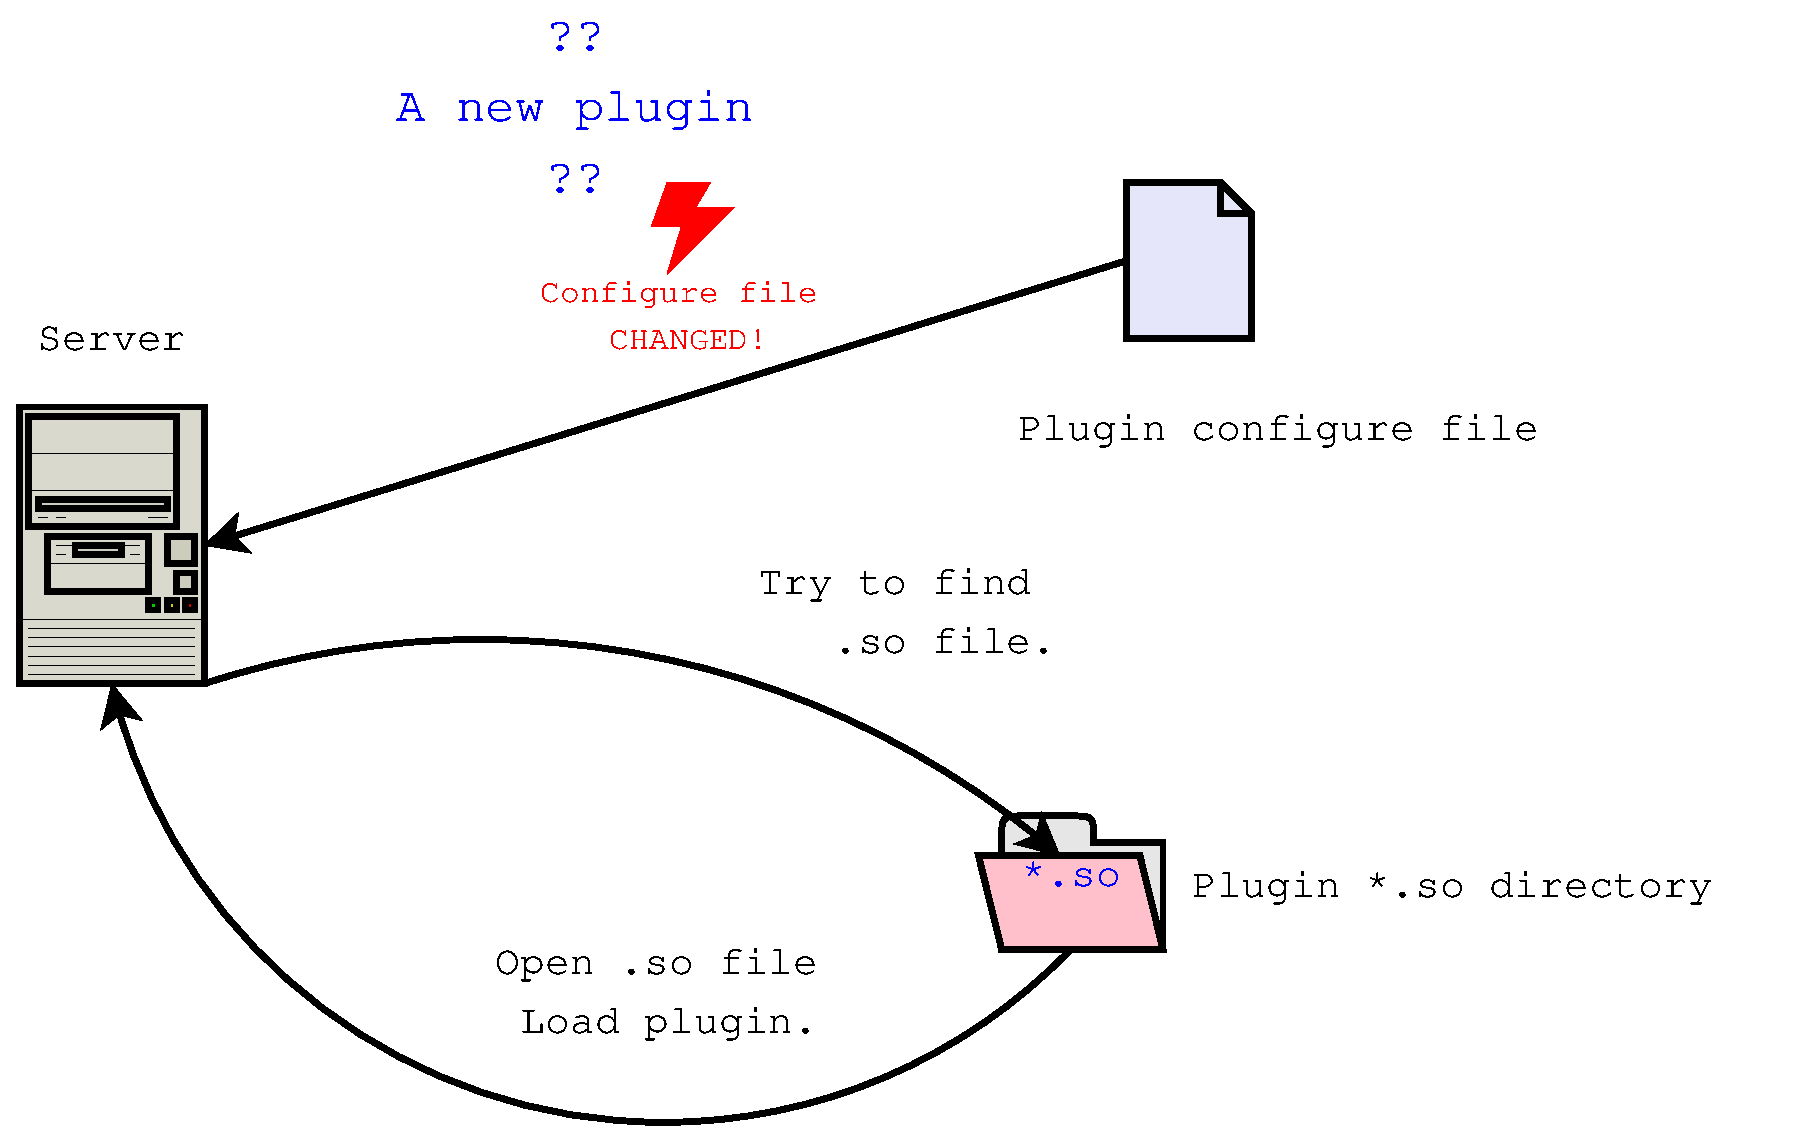
\includegraphics[height=8cm, width=13cm]{pics/loadplugin.eps}
	\caption{动态加载过程}
	\label{loadplugin}
	\end{figure}
	
	插件的加载和插件的调用是异步进行的。因此,在加载插件的时候,必须对插件的核心数据加锁,避免出现数据错乱导致服务器崩溃。
	
	动态链接技术可以选择性的加载共享库,也就是说,在程序的运行过程中,程序可以在任意时刻加载任意的共享库。动态链接技术的这个特点可以用来实现插件的加载。在服务器监测到插件的增加之后,通过配置文件中的信息,检索到插件的共享库,利用动态链接技术,将插件的共享库加载到内存中,并通知服务器插件接口的地址。服务器得到这些信息之后,就可以对插件进行调用。

\section{服务器的分析和设计}
\subsection{I/O分析和设计}
	Web服务器是I/O密集型的程序。在运行的大部分时间中,服务器都在进行这I/O处理。这些I/O处理包括接收和发送网络数据,读取和写入磁盘数据等。因此,服务器I/O效率的高低直接决定这服务器运行效率的高低。服务器在处理连接请求的时候,通常在某一时刻要同时处理多个请求,但这些请求并不是同时需要进行I/O。当某一个请求在等待I/O事件时,将这个请求暂时不处理,直到I/O事件发生再进行处理。在这个过程中,服务器对需要I/O的请求进行处理。这样可以增加服务器的吞吐量,提高效率。
	
	在本系统中,服务器的I/O处理采用非阻塞I/O+I/O多路复用+线程池的模式。对于所有的描述符,都将其设置为非阻塞模式,并通过I/O多路复用监测描述符的I/O事件。一旦某个描述符需要进行I/O,那么从线程池中获得一个线程,在这个线程中运行描述符对应的I/O处理函数。如果多个描述符同时需要I/O,可以实现并行处理,提高效率。I/O的结构图如图\ref{IO}。
	
	\begin{figure}[htbp]
	\centering
	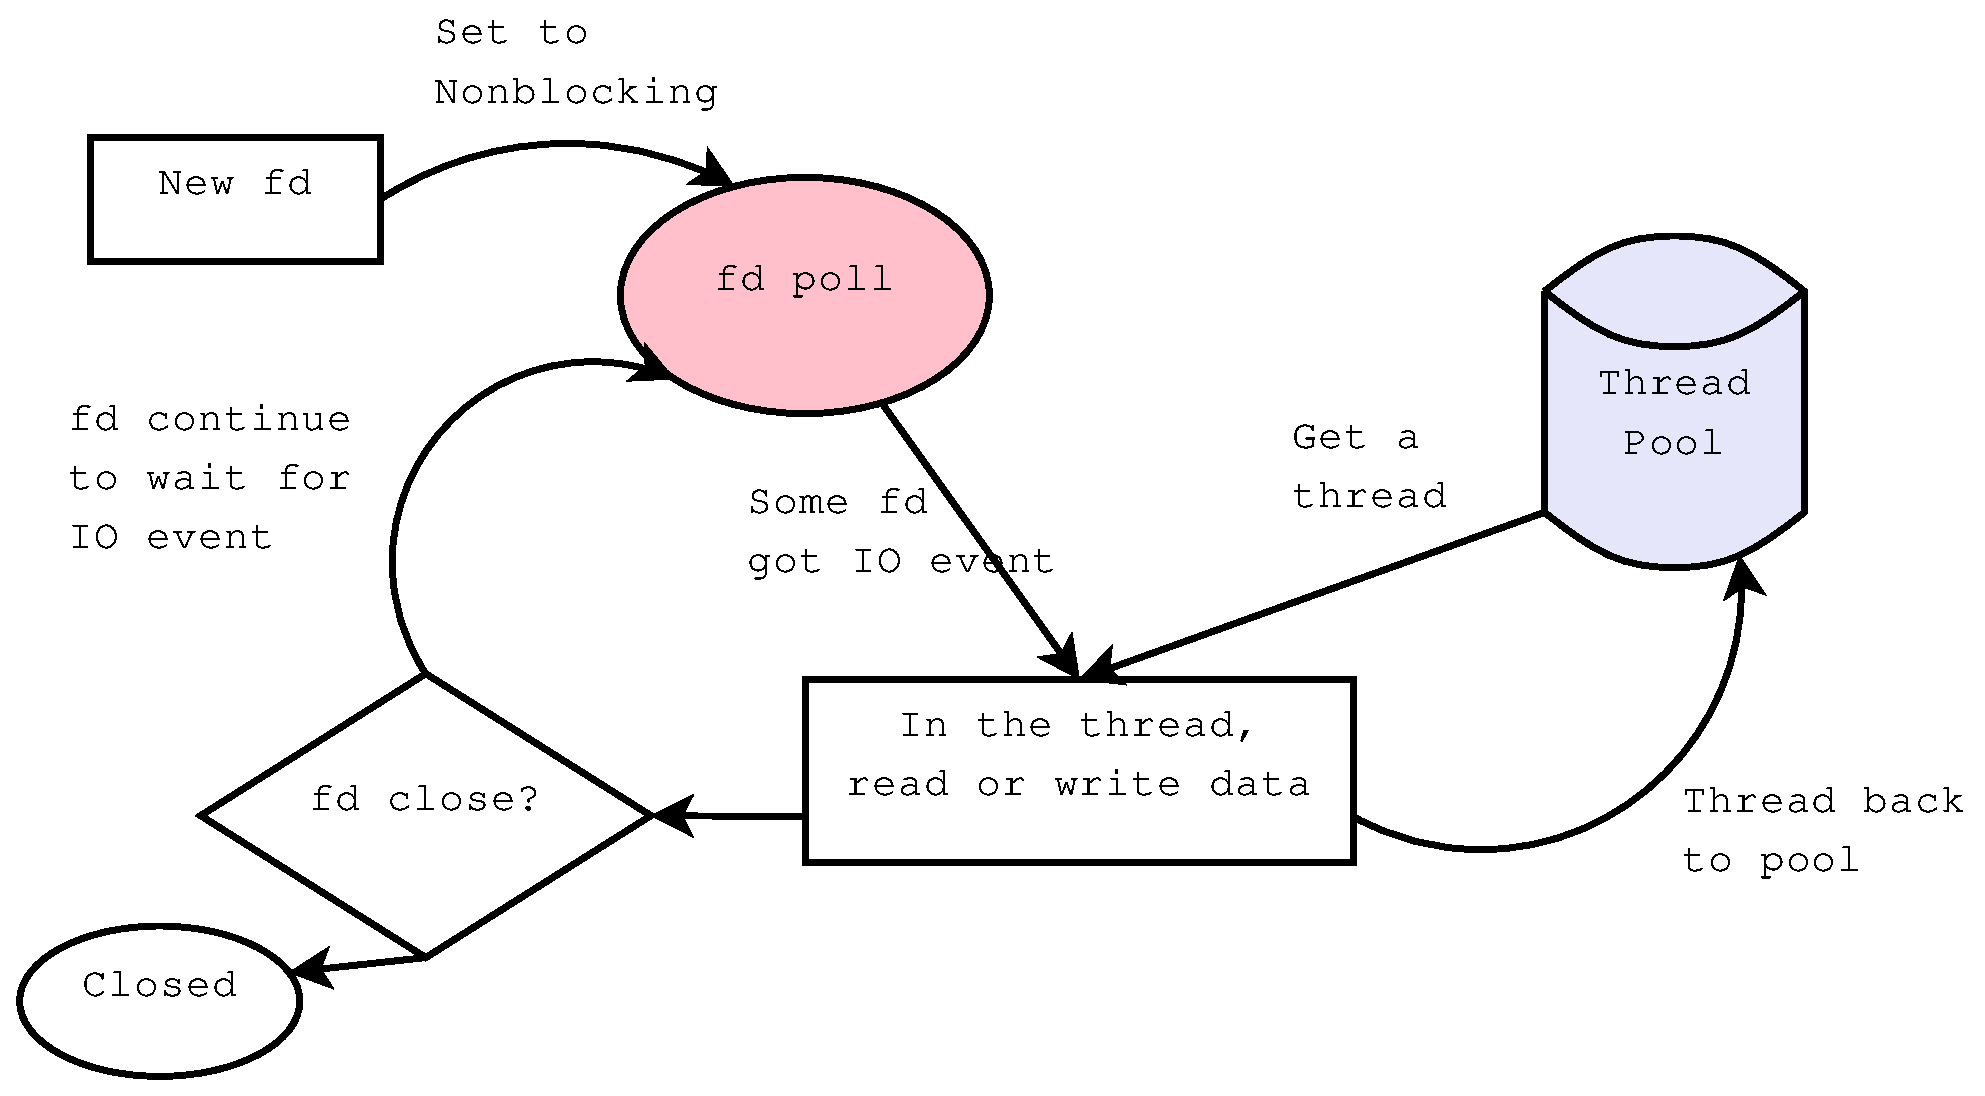
\includegraphics[height=8cm, width=15cm]{pics/IO.eps}
	\caption{I/O结构图}
	\label{IO}
	\end{figure}
	
\subsection{线程池的分析和设计}
	为了实现线程池的目的,必须能够控制线程使其在没有任务执行的时候处于等待状态(或者睡眠状态),而当有任务需要线程处理的时候,又可以快速的使线程恢复运行。当然,这里的运行只线程处于可运行状态(Running),是否真正运行要看线程调度程序对线程的调度。
	
	线程池具有如下特点:
	\begin{itemize}
		\item 在线程池的初始化阶段,预创建一些线程放入线程池中。
		\item 当线程池中没有可用线程时候,创建一个新的线程。这个新线程运行完任务之后,被加到线程池中,等待下一次调用。
		\item 当线程的总数量达到某一个最大值的时候,线程池将不在创建新的线程。如果此时没有可用线程,则请求线程的调用将阻塞,直到有线程可以使用。
		\item 当空闲线程较多时,将适当的销毁一些线程。通常,保证空闲线程的数量不会大于总的线程数量的2/3。
		\item 创建一个管理线程,对线程池进行管理。包括统计线程池的各种数据,销毁过多的空闲线程等。
	\end{itemize}
	
	在Linux下,使用Pthread库对线程进行创建管理等操作。Pthread库中的条件变量(Condition Variables)可以用来实现控制线程运行和等待的目的。条件变量可以使线程一直处于睡眠状态直到一些事件发生(或者条件改变)\ucite{unp}。线程处在一个循环中,循环的还是调用pthread\_cond\_wait等待有任务可以运行。此时,线程处于sleep状态。当有任务需要处理时,线程池调用pthread\_cond\_signal告诉线程有任务可以运行,唤醒线程。随后,线程处理任务。任务结结束后,线程再次回到sleep状态。线程的状态改变可用图\ref{tpthread}表示。
	
	\begin{figure}[htbp]
	\centering
	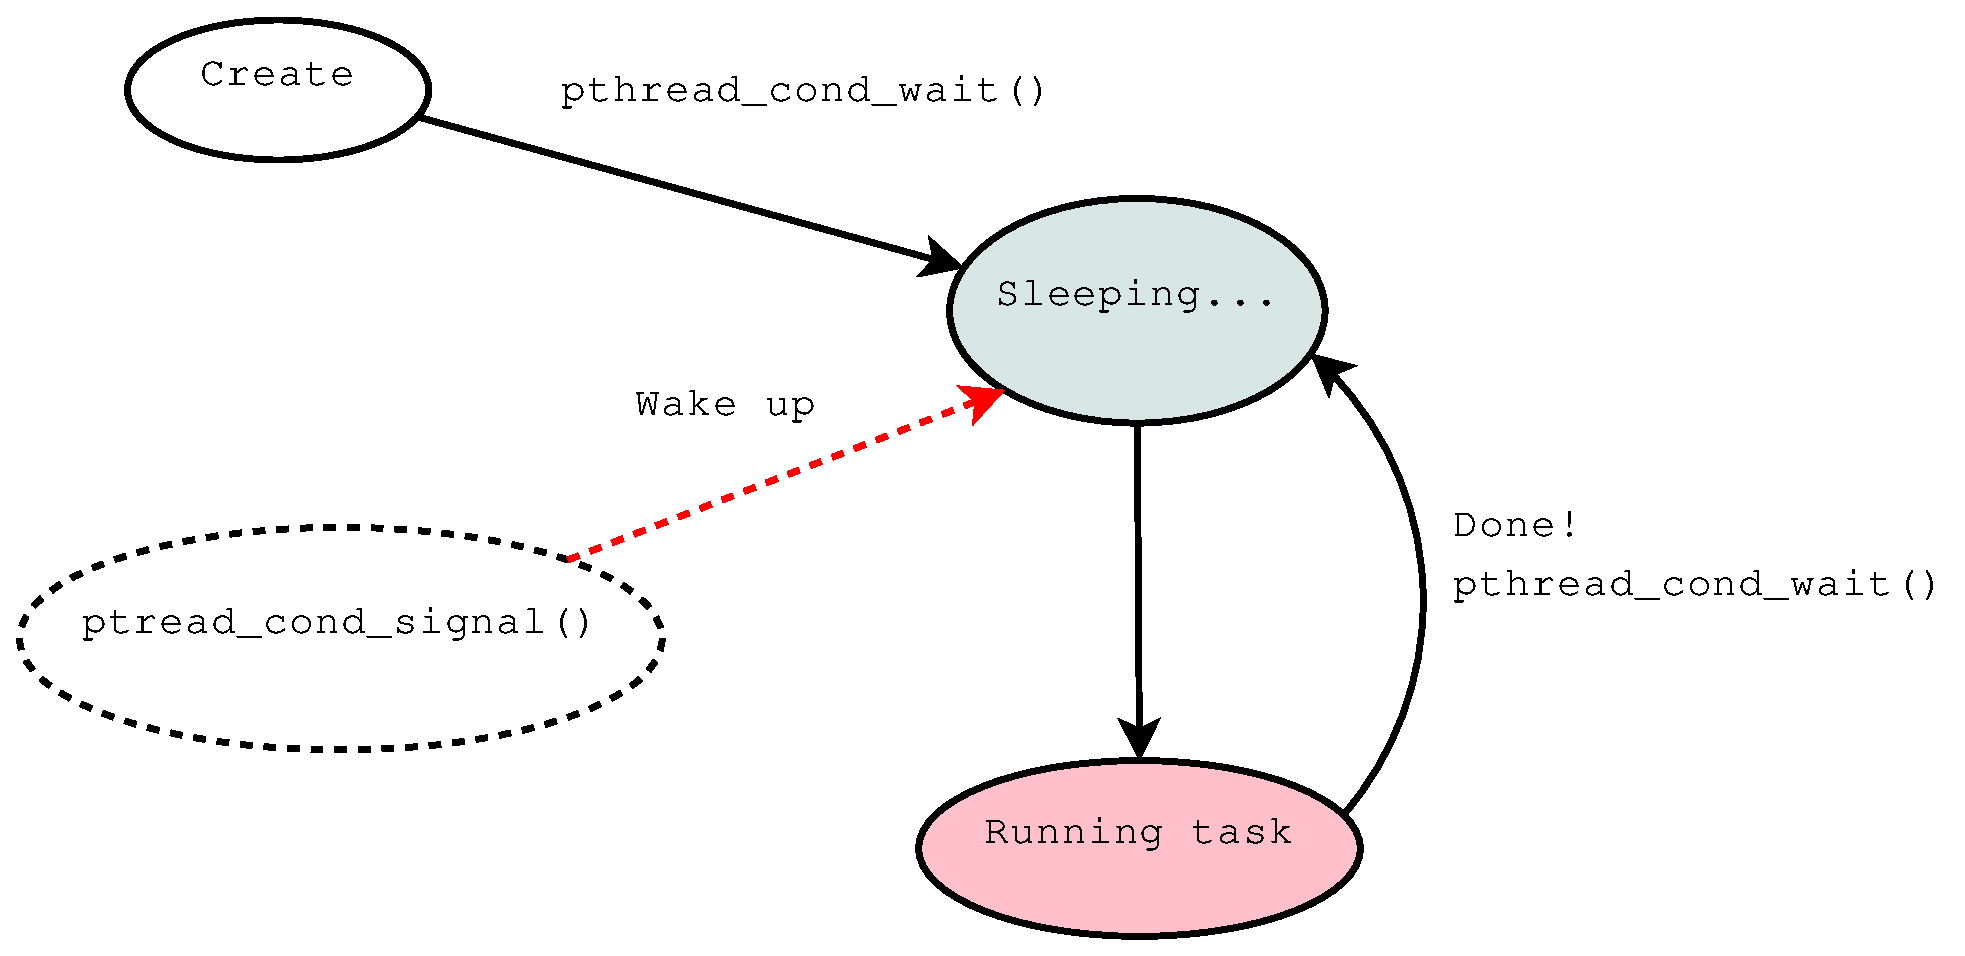
\includegraphics[height=6cm, width=13cm]{pics/tpthread.eps}
	\caption{线程状态图}
	\label{tpthread}
	\end{figure}
	
\subsection{连接处理状态机的分析和设计}
	对于每一个请求,在不同的时刻,对请求所处在的状态进行定义。根据HTTP协议的规定,对于服务器而言,请求经历了读取Reqeust,解析Request,读取POST数据,处理连接请求,创建Response,发送Response回客户端这几个状态。为了便于处理,在请求的生命周期中增加了几个状态,最后的状态图如图\ref{state}。
	\begin{figure}[t]
	\centering
	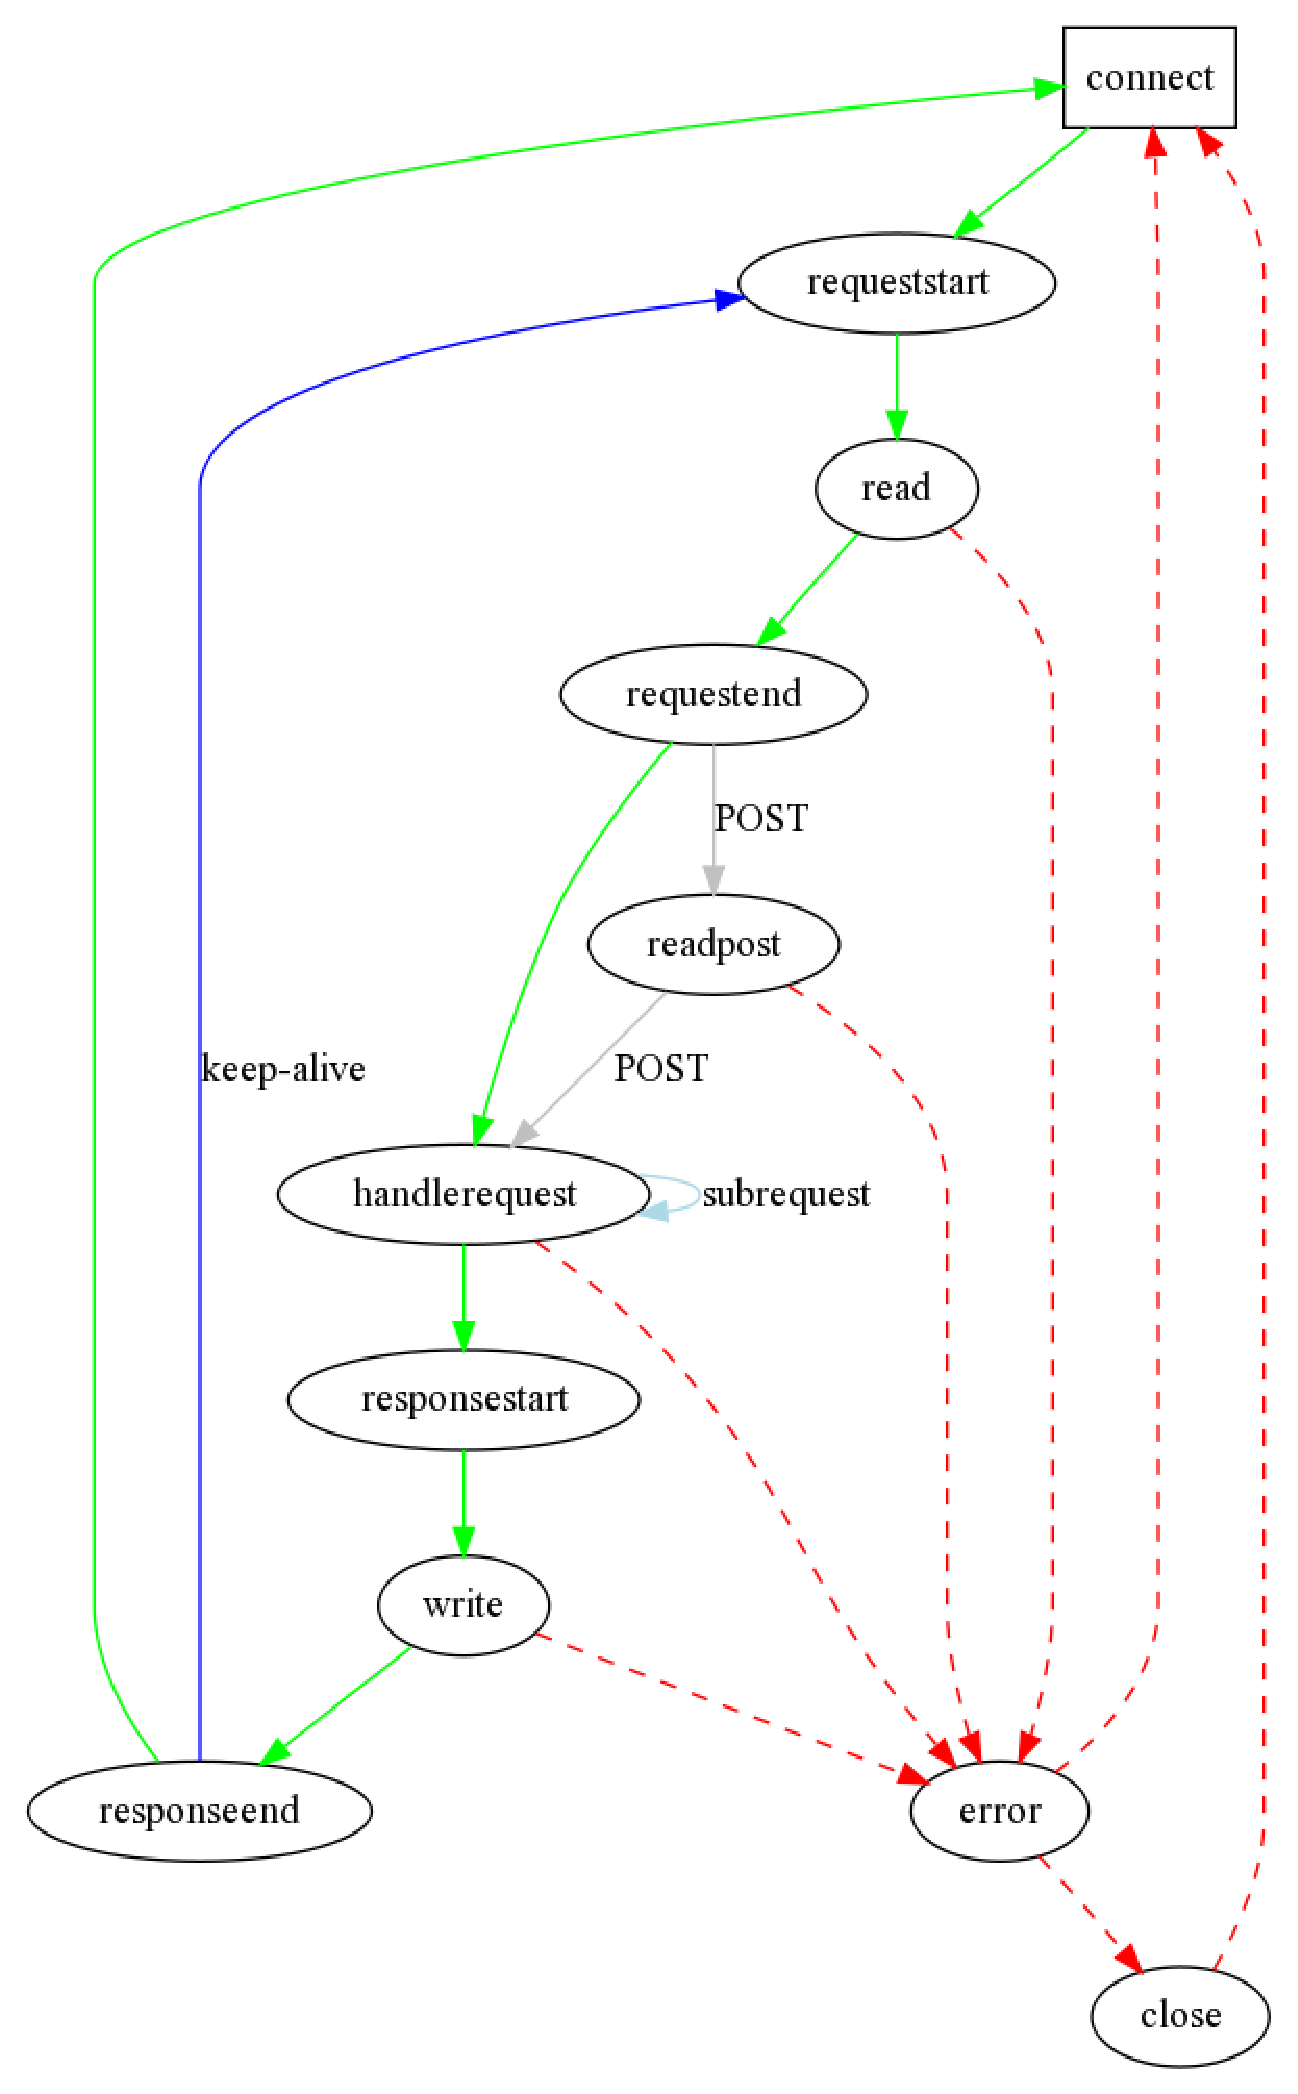
\includegraphics[height=16cm, width=12cm]{pics/state.eps}
	\caption{请求处理状态图}
	\label{state}
	\end{figure}
	
	总共定义了10状态(图中椭圆所示)。connect状态是一个比较特殊的状态,它并不是请求在某一时刻的状态,它仅仅是用来标记连接对应的结构体可以使用。这个状态用来进行内部的数据处理,不参与请求的处理。
	
	各个状态的含义:
	\begin{itemize}
		\item connect: 标记connection结构体可用。
		\item requeststart: 请求开始。主要做一些时间的记录工作。
		\item read: 读取Request数据。
		\item handlerequest: 解析Request数据。
		\item requestend: 解析结束。做一些解析的收尾工作。
		\item readpost: 读取POST数据。如果没有POST数据,跳过此状态。
		\item responsestart: 处理请求。在这个状态中调用插件。这也是最重要的状态。
		\item write: 发送数据回client。
		\item responseend: 处理结束。做最后的清理工作。
		\item error: 出错。设置错误信息。
		\item close: 连接关闭。
	\end{itemize}
	
	图\ref{state}中虚线表示错误处理流程。一旦处理出错,服务器将关闭连接,不在接收这个连接的其余的请求。
	
	responseend状态结束后有两条路径:一条是标有keep-alve的指向requeststart状态的路径,一条是指向connect的路径。对于HTTP/1.1,通常是持久连接(Persistent Connection),也就是说,在处理完一个请求之后,连接不关闭。在此连接上可以再进行多次请求,直到连接双方有一方关闭了连接。如果连接不是持久连接,那么在处理完请求之后,服务器关闭连接。此时,请求已经处理完毕,不再需要任何状态表示。但是,为了方便内部数据的处理,将连接对应的结构体标记为connect状态。当有新的连接时,可以重新使用这个结构体。
	
	当请求处于handlerquest状态时,可能还需要进行子请求。这时候,请求依然处于handlerquest状态,并在这个状态中对子请求进行处理。某些请求可能会有多个子请求。这时,请求会一直停留在这个状态,处理所有子请求,然后进入下一个状态。
	
\section{本章小结}
	本章包括动态扩展功能接口的分析设计和服务器的分析设计。
	
	在动态扩展功能接口的分析和设计中,首先通过分析HTTP协议,根据HTTP协议的处理过程,设计动态扩展功能接口的调用过程。然后,根据HTTP协议的数据格式,设计接口函数。最后,根据动态链接技术,设计出动态加载功能的过程。
	
	在服务器的分析和设计中,通过对I/O,线程池和连接处理状态机三个主要部分的分析和设计,构建出服务器的主体框架,完成服务器关键部分的设计。I/O使用非阻塞I/O和I/O多路复用,配合线程池提高服务器的I/O效率。对连接请求的生命周期进行划分,设计出连接的各个状态,通过状态机完成对连接的处理。
	
\chapter{动态扩展功能接口和服务器的实现和测试}

	基于上一章的分析和设计,本章描述了动态扩展功能接口和服务器的实现,最后给出了测试的结果。动态扩展功能接口的实现主要描述了接口定义的实现,加载过程的实现和调用过程的实现。在服务器的实现中重点描述了I/O,连接处理状态机和线程池的实现

\section{动态扩展功能接口的实现}

\subsection{动态扩展功能接口定义的实现}
	为了对插件进行描述,通过plugin结构体对插件进行封装。plugin结构体使用C语言的struct实现,包含有插件的所有信息。包括版本,名称,一系列接口函数指针以及一些辅助的数据成员。plugin结构体可以用图\ref{plugin_s}描述。
	
	\begin{figure}[htbp]
	\centering
	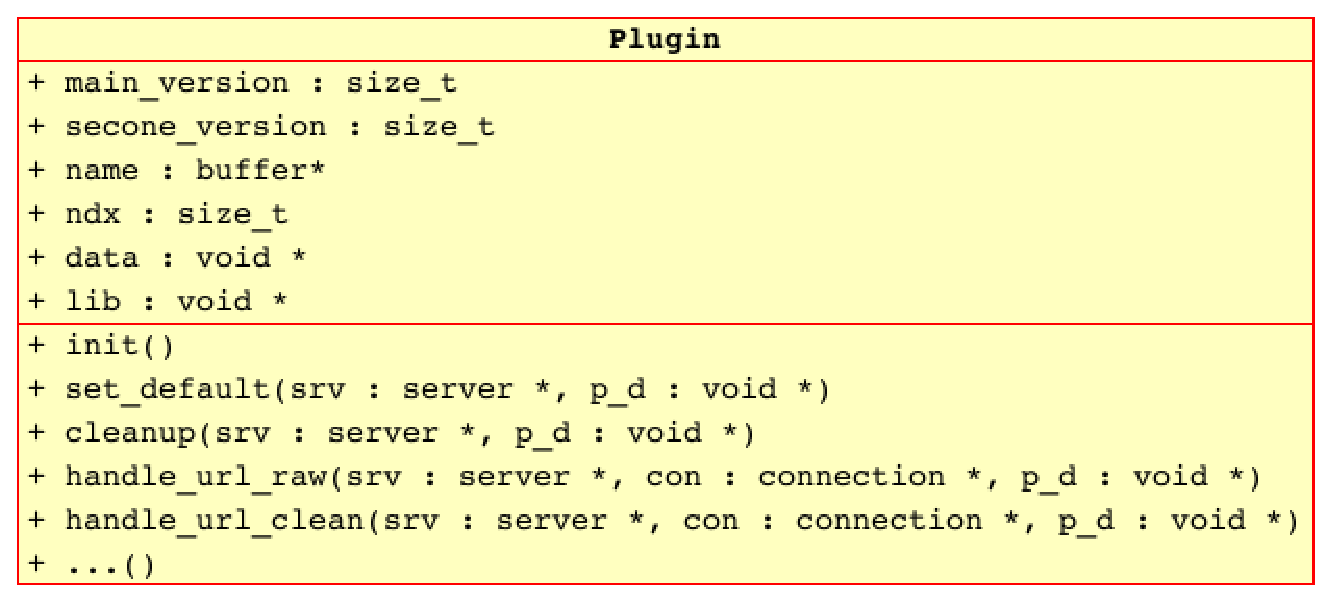
\includegraphics[height=6cm, width=12cm]{pics/plugin_s.eps}
	\caption{plugin结构体定义}
	\label{plugin_s}
	\end{figure}
	
	其中,main\_version和second\_version数据成员分别表示插件的主版本号和次版本号。服务器在加载插件的过程中,要对这两个版本号依据版本控制的规则进行检查。如果版本不兼容,则服务器不对插件进行加载,同时在日志文件中提示插件版本不兼容。
	
	name用来保存插件的名称。data指向插件自己使用的数据,和后面的函数指针中的p\_d参数对应。插件在初始化的过程中要自己分配所需要的数据空间,然后将地址赋给data。插件卸载时,要对这个数据空间进行释放。后面的一系列的函数指针保存着插件对应的函数的入口地址。每一个插件都要定义一个结构体plugin\_data用来存储插件所使用的私有数据。这个结构体的名称必须是plugin\_data,且在定义的开始部分一定是宏:PLUGIN\_DATA。插件在初始化的时候,要将这个结构体实例化并将其指针赋给plugin结构体中的data成员。宏PLUGIN\_DATA定义了一些数据成员。通过这一硬性规定,所有的插件的私有数据空间的开始部分都包含PLUGIN\_DATA所定义的数据成员。同时,插件系统自己也定义了一个plugin\_data结构体,这个结构体中只包含PLUGIN\_DATA定义的数据成员。插件系统通过把插件的数据空间强制转换成自己定义的plugin\_data结构体类型,就可以访问插件中这些有PLUGIN\_DATA定义的数据,从而实现对插件的一些管理。
	
	对于服务器而言,无论系统中有多少插件并且插件的接口实现个数都不相同,对于每个请求,服务器按部就班的调用所有插件接口函数。对于插件中的每一个接口函数,插件系统也定义了一些列的接口函数用于服务器调用插件。在调用插件时,服务器仅仅能看到这些接口,至于插件系统中到底有多少插件,服务器无法也不必知道。这些接口的定义如下:
	
\begin{verbatim}
handler_t plugin_handle_url_raw(server *srv, connection *con);
handler_t plugin_handle_url_clean(server *srv, connection *con);
handler_t plugin_handle_docroot(server *srv, connection *con);
handler_t pluginhandle_physical(server *srv, connection *con);
handler_t plugin_handle_connection_close(server *srv, connection *con);
handler_t plugin_handle_joblist(server *srv, connection *con);
handler_t plugin_handle_subrequest_start(server *srv, connection *con);
handler_t plugin_handle_handle_subrequest(server *srv, connection *con);
handler_t plugin_handle_request_end(server *srv, connection *con);
handler_t plugin_handle_connection_reset(server *srv, connection *con);
handler_t plugin_handle_trigger(server *srv);
handler_t plugin_handle_cleanup(server *srv);
\end{verbatim}

	在这些函数中,对每个插件的对应的接口函数进行调用。如果插件没有实现对应的接口函数,怎将忽略之。由于服务器无法判断当前连接是否需要使用某个插件来处理。因此,在这些函数中,通常都是逐个的调用系统所有插件的对应的函数,然后根据这些函数的返回值,判断是否需要继续调用其他插件的对应函数还指直接处理结束。
	
\subsection{动态加载过程的实现}
	首先,定义插件的配置文件。插件的配置文件名字是固定的:swiftd-plugin.conf。插件配置文件存放的位置可以在服务器的配置文件中进行设置。配置文件的形式为”插件名称:插件动态库文件所在目录的绝对路径\$“。每一个插件,在配置文件中都有单独一行的这种形式的配置信息。例如:

\begin{verbatim}
#以#开头的行为注释。swiftd-plugin.conf
#每个插件一行,每个插件配置信息必须以"$"结尾。
dir_index:/home/hcy/plugins/$
cgi:/home/temp/plugins/$
...
\end{verbatim}

	这个例子中定义了两个插件:dir\_index和cgi。它们存放的位置分别是 /home/hcy/plugins/ 和 /home/temp/plugins/ 。
	
	插件的动态库的名称必须为:插件名称 +.so。服务器读取到插件配置信息之后,根据配置文件中的插件名称,可以确定插件的动态库的名称。这样就可以得到插件动态库的绝对路径。例如,上面两个插件的绝对路径分别为/home/hcy/plugins/dir\_index.so和/home/temp/plugins/cgi.so。
	
	服务器使用Linux平台下的Inotify技术对插件配置文件进行监测。Inotify产生一个文件描述符,通过监测这个文件描述符是否有数据可读即可监测到文件的改变。由于Inotify是根据文件描述符的有无数据可读来判断文件是否发生了改变。因此,可以将Inotify的描述符设置成非阻塞模式,然后利用服务器中的I/O多路复用来监测其描述符的I/O事件 。这样,可以实现对配置文件修改的异步实时监测,同时,也不会影响服务器的效率。监测过程如图\ref{inotify}。
	
	\begin{figure}[htbp]
	\centering
	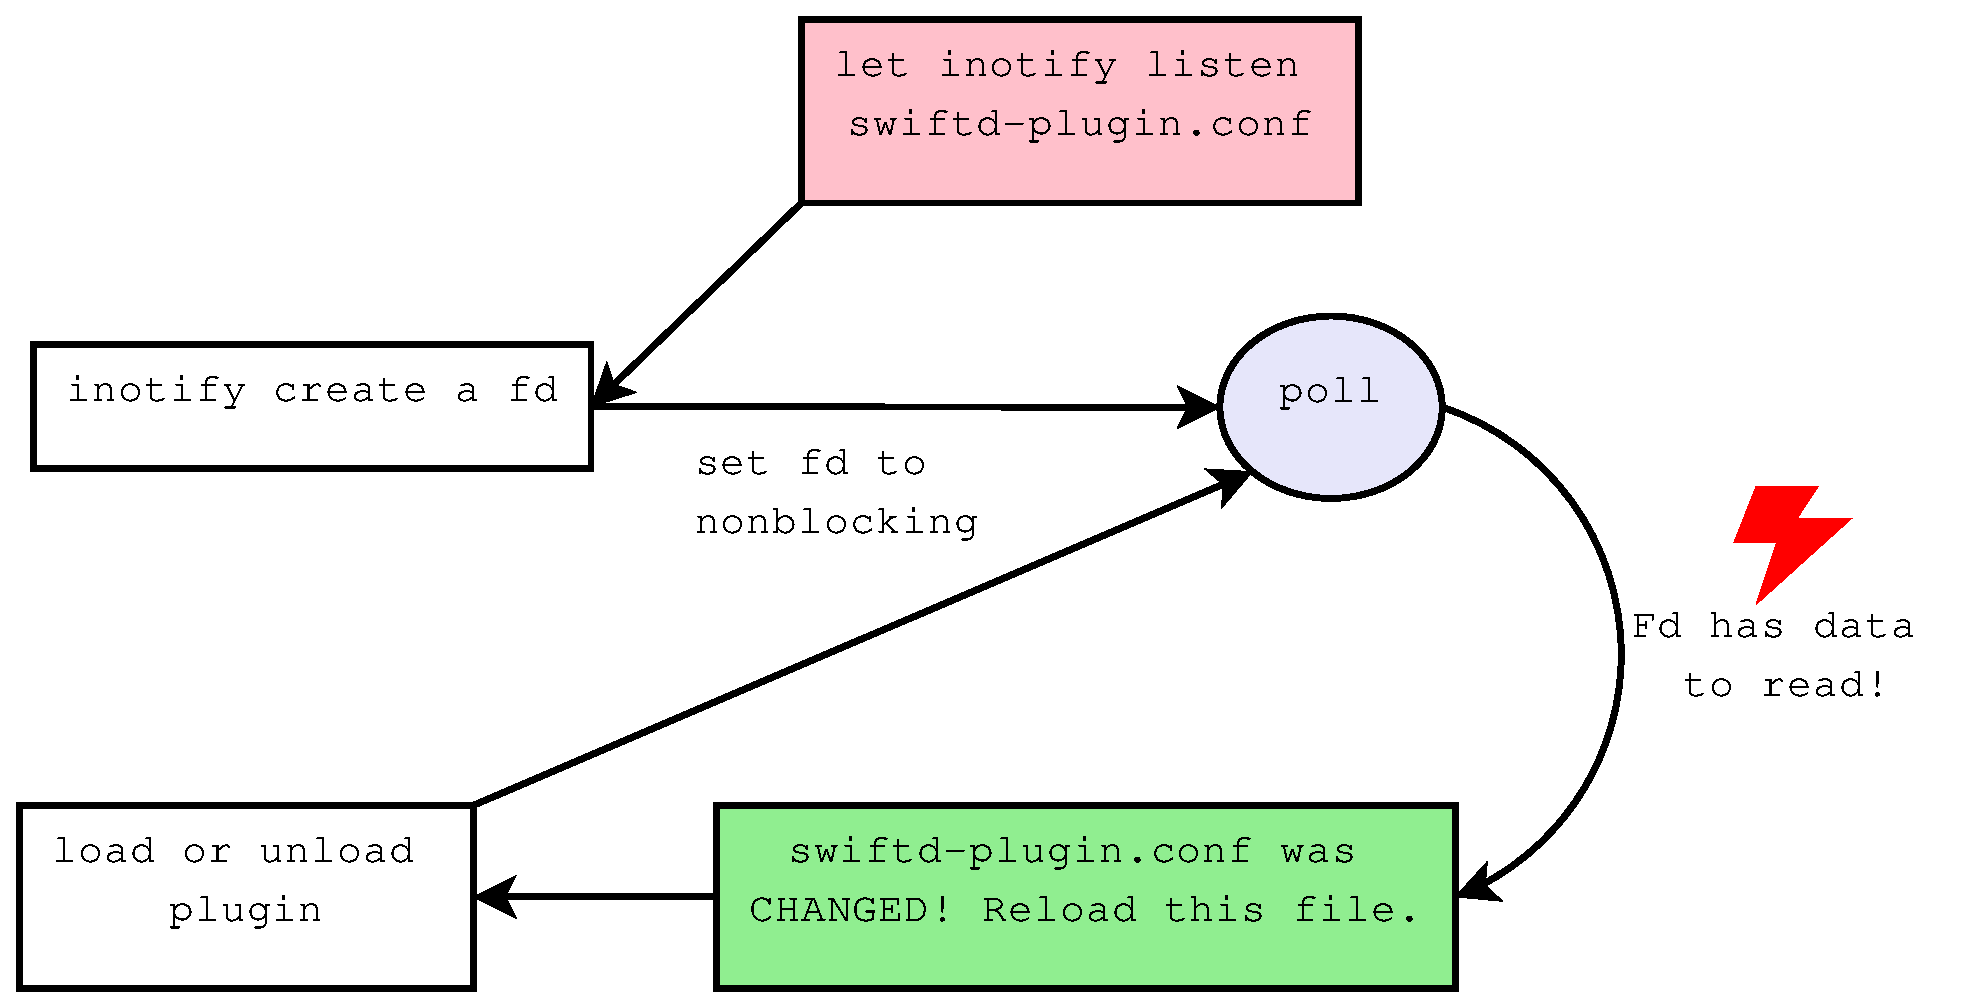
\includegraphics[height=8cm, width=15cm]{pics/inotify.eps}
	\caption{Inotify监测过程}
	\label{inotify}
	\end{figure}
	
	\begin{enumerate}
		\item 在服务器初始化阶段,调用inotify\_init()创建一个Inotify实例。此时函数返回一个文件描述符fd。
		\item 调用inotify\_add\_watch()对插件配置文件所在的目录监测IN\_CLOSE\_WRITE事件(参见后文)。
		\item 将inotify\_init()返回的文件描述符fd和对应的I/O事件处理函数\\plugin\_conf\_inotify\_fdevent\_handler()注册到I/O多路复用系统中。由I/O多路复用监测fd的I/O事件。
		\item 配置文件被修改。调用fd的I/O事件处理函数。在这个处理函数中重新加载所有插件。
		\item fd重新进入等待I/O事件状态。
	\end{enumerate}
	
	对于有些编辑器(如,vi),在对文件进行编辑的时候并不是在原文件上进行修改,而是首先复制一个文件的副本,然后在这个副本上进行编辑操作。当编辑完毕之后,用这个副本覆盖原来的文件。如果直接监测对应文件的IN\_MODIFY事件,那么,在进行文件覆盖时,监测到文件被删除,Inotify将停止对文件的监测,也就是相当于inotify\_rm\_watch文件了。这样,就只能监测到一次IN\_DELETE\_SELF事件。随后什么也监测不到。为了能够对文件进行正常的监测,这里不直接监测文件,而监测包含文件的文件夹。一旦文件被覆盖,将触发文件夹IN\_CLOSE\_WIRTE事件。这样即可得到文件的修改事件。
	
	当服务器检测到了配置文件的修改之后,服务器执行下面的函数完成插件的加载。这个函数被注册到I/O多路复用系统中,有多路复用系统在检测到配置文件修改后调用。
	
	\begin{verbatim}
static handler_t plugin_conf_inotify_fdevent_handler(
				void *srv, void *ctx, int revents)
{
	server *s = (server*)srv;
	conf_inotify *ity = (conf_inotify*)ctx;
	//分配存储空间ity-> buf
	...
	
	int rlen, offset = 0;
	int read_done = 0;
	while(!read_done)
	{
		if(-1 == (rlen = read(ity -> fd
			, ity -> buf + offset
			, ity -> buf_len - offset))){
			...
		}
		else{
			offset += rlen;
		}
	}
	int tmp_len;
	struct inotify_event *e;
	for(tmp_len = 0; tmp_len < offset; )
	{
		e = (struct inotify_event *)
				(ity -> buf + tmp_len);
		if(e -> wd == ity -> plugin_conf_wd)
		{
			if(e -> mask & IN_CLOSE_WRITE)
			{
				pthread_mutex_lock(
					&s -> plugin_lock);
				plugin_free(s);
				pthread_mutex_unlock(
					&s -> plugin_lock);
				plugin_load(s);
			}
			break;
		}
		tmp_len += sizeof(int); 			
		tmp_len += 3 * sizeof(uint32_t);	
		tmp_len += e -> len;
	}
	
	return HANDLER_FINISHED;
}
	\end{verbatim}
	
	在函数中,通过read从inotify系统中读取发生的修改事件,判断所发生的事件是不是IN\_CLOSE\_WRITE。最后,释放以前加载的所有插件,调用plugin\_load重新加载所有的插件,包括新增加的。
	
	为了能对插件进行初始化并得到其所实现的接口函数的入口地址。规定所有的插件中必须实现一个函数XXX\_init,其中,	XXX为插件的名称(必须为插件配置文件中的名称)。这个函数的原型为:
	
\begin{verbatim}
        void XXX_init(plugin *p)
\end{verbatim}

	在这个函数中,主要而且必须的工作就是对所传进来的plugin结构体的数据成员进行赋值。其中,最重要的是版本和接口函数指针的赋值。如果插件没有实现某一个接口函数,那么那么接口函数对应的函数指针必须赋值为NULL。这点很重要。在插件系统得到了插件动态库的路径之后,通过dlopen调用将动态库加载到内存中。然后,插件系统通过dlsym调用获得插件对应的XXX\_init函数的入口地址。接着插件系统创建一个plugin结构体的实例,并以这个实例的地址为参数调用刚才得到的XXX\_init函数。至此,插件系统得到了插件的所有信息。完成了插件的加载工作。
	
\subsection{动态扩展功能接口调用的实现}

	首先,为了对插件的各个接口进行标记,程序中定义了一个枚举类型plugin\_slot\_t。定义如下:
\begin{verbatim}
typedef enum
{
	PLUGIN_SLOT_SET_DEFAULT= 0,
	PLUGIN_SLOT_CLEANUP,
	PLUGIN_SLOT_TRIGGER,
	PLUGIN_SLOT_SIGHUP,
	PLUGIN_SLOT_URL_RAW,
	PLUGIN_SLOT_URL_CLEAN,
	PLUGIN_SLOT_DOCROOT,
	PLUGIN_SLOT_PHYSICAL,
	PLUGIN_SLOT_JOBLIST,
	PLUGIN_SLOT_CONNECTION_CLOSE,
	PLUGIN_SLOT_CONNECTION_RESET,
	PLUGIN_SLOT_SUBREQUEST_START,
	PLUGIN_SLOT_HANDLE_SUBREQUEST,
	PLUGIN_SLOT_SUBREQUEST_END,
	PLUGIN_SLOT_SIZE, 			//slot的数量。
}plugin_slot_t;
\end{verbatim}

	这个枚举类型中的值与接口函数有这对应关系。从这些值的名称中可以得知。比如,PLUGIN\_SLOT\_DOCROOT对应于docroot接口函数。
	
	然后,为了提高插件的调用效率,对每一个插件进行登记造册。plugin\_slot是一个void *类型的二维数组,相当于plugin的登记表。当插件加载之后,插件所有的信息都存放在对应的plugin结构体中。插件系统遍历所有的plugin结构体,对插件所实现的接口方法进行登记(前面已经说过,对于没有实现的插件接口,插件必须将对应的函数指针赋值为NULL。这就可以帮助插件系统判断插件到底实现了哪些接口函数)。
	
	plugin\_slot虽说是一个void*类型的数组,但是其存放的是plugin结构体的插件。plugin\_slot数组的每一行对应一个接口函数。对应关系由plugin\_slot\_t枚举类型确定。比如,根据C语言语法规定,枚举值PLUGIN\_SLOT\_DOCROOT等于6。那么docroot接口函数对应的行就是第7行(C语言从第0行开始计算),换句话说,第7行中保存这所有实现了docroot接口函数的插件的plugin结构体指针。
	
	例如,目前有三个插件,它们登记之后plugin\_slot数组的情况可有表\ref{example_plugin}表示。
	\begin{table}[htbp]
	\caption{plugin\_slot示例:}
	\label{example_plugin}
	\centering
	\begin{tabularx}{\textwidth}{p{6cm}XXXl} %最后一列是空的。这样可以是倒数第二列居中,否则会报错或不居中。
	\toprule
	\centering 名称 & \centering  插件1 & \centering  插件2 &\centering 插件3&\\
	\midrule
	\centering PLUGIN\_SLOT\_PHYSICAL &\centering  p1 &\centering  p2 &\centering  p3&\\
	\centering PLUGIN\_SLOT\_URI\_CLEAN &\centering  p1 &\centering  p2 &\centering  p3&\\
	\centering PLUGIN\_SLOT\_DOCROOT &\centering  p1 & \centering NULL & \centering NULL&\\
	\bottomrule
	\end{tabularx}
	\end{table}
	
	NULL表示插件没有实现对应的接口函数。px表示插件对应的plugin结构体指针。
	
	表\ref{example_plugin}中仅仅示例了三个接口函数。从表\ref{example_plugin}可以看出,插件1实现了全部的三个接口函数,插件2没有实现第三个接口函数,插件3和插件2一样。插件系统利用如下的宏对插件进行登记:
	
\begin{verbatim}
#define PLUGIN_REGISTER_SLOT(x, y)\
 for(i = 0; i < srv -> plugins -> used; ++i)\
 {\
  plugin *p = srv -> plugins -> ptr[i];\
  if(p -> handle_##y)\
  {\
   log_error_write(srv, __FILE__, __LINE__, \
   			"sb", "slot: ", p -> name);\
   if(NULL == srv -> slots -> size)\
   {\
    srv -> slots -> used = (size_t *)\
    		calloc(PLUGIN_SLOT_SIZE, sizeof(size_t *));\
    srv -> slots -> size = (size_t *)\
    		calloc(PLUGIN_SLOT_SIZE, sizeof(size_t *));\
	srv -> slots -> ptr = (void ***)\
		calloc(PLUGIN_SLOT_SIZE, sizeof(void **));\
   }\
   if (srv -> slots -> size[x] == 0)\
   {\
	srv -> slots -> size[x] = 8;\
	srv -> slots -> ptr[x] = (void **)\
		calloc(srv -> slots -> size[x], sizeof(void *));\
   }\
   else if (srv -> slots -> size[x] \
   		== srv -> slots -> used[x])\
   {\
	srv -> slots -> size[x] += 8;\
	srv -> slots -> ptr[x] = (void **)realloc(\
			srv -> slots -> ptr[x],\
			srv -> slots -> size[x] * sizeof(void *));\
   }\
   srv -> slots -> ptr[x][srv -> slots -> used[x]] = (void*)p;\
   ++srv -> slots -> used[x];\
  }\
 }
\end{verbatim}

	宏的第一个参数x确定需要登记的接口函数的类型,这个参数是plugin\_slot\_t类型。第二个参数y是x对应的接口函数在pluing结构体中对应的数据成员的名称不包含开头的handle\_。宏中扫描所有的插件,如果插件实现了x对应的接口函数,就将这个插件对应的plugin结构体指针存入plugin\_slot数组中。宏中还包含了对plugin\_slot数组空间申请。
	
	例如,这个宏调用实现对docroot接口函数的登记工作。
\begin{verbatim}
	PLUGIN_REGISTER_SLOT(PLUGIN_SLOT_DOCROOT, handle_docroot);
\end{verbatim}

	得到这张登记表之后,基本上所有的操作都是围绕这个表来进行的。插件系统定义了下面的宏,这个宏用来作为模板,实现先前提到的插件系统提供给服务器的那一些列接口函数。而这些接口函数是服务器调用插件的关键。
\begin{verbatim}
#define PLUGIN_CALL_HANDLER(x,y)\
 handler_t plugin_handle_##y(server *srv, connection *con)\
 {\
  if (NULL == srv || NULL == con)\
  {\
   return HANDLER_ERROR;\
  }\
   \
  if (!srv -> slots -> ptr)\
  {\
   return HANDLER_GO_ON;\
  }\
  if (!srv -> slots -> ptr[x])\
  {\
   return HANDLER_GO_ON;\
  }\
   \
   pthread_mutex_lock(&srv -> plugin_lock);\
   plugin *p;\
   size_t i;\
   handler_t ht;\
   for (i = 0; i < srv -> slots -> used[x]; ++i)\
   {\
	if (srv -> slots -> ptr[x][i])\
	{\
	 p = (plugin*)srv -> slots -> ptr[x][i];\
	 switch(ht = p -> handle_##y(srv, con, p -> data))\
	 {\
	  case HANDLER_GO_ON:\
	    break;\
	  case HANDLER_FINISHED:\
	  case HANDLER_COMEBACK:\
	  case HANDLER_WAIT_FOR_EVENT:\
	  case HANDLER_ERROR:\
	  case HANDLER_WAIT_FOR_FD:\
		pthread_mutex_unlock(&srv -> plugin_lock);\
		return ht;\
	  default:\
		log_error_write(srv, __FILE__, __LINE__, \
				"Unknown handler type.");\
		pthread_mutex_unlock(&srv -> plugin_lock);\
		return HANDLER_ERROR;\
	  }\
     }\
   }\
   pthread_mutex_unlock(&srv -> plugin_lock);\
   return ht;\
 }
\end{verbatim}	

	宏的第一个参数x确定需要登记的接口函数的类型,这个参数是plugin\_slot\_t类型。第二个参数y是x对应的接口函数在pluing结构体中对应的数据成员的名称不包含开头的handle\_。在这个宏中,通过x确定pluing\_slot数组的行,依次调用这行中存储的plugin结构体的对应的成员函数(函数指针)。这些成员函数的名称有y确定。这一调用工作,正是插件系统提供给服务器的所有接口函数的全部工作。利用这个宏,可以模板化的实现所有这些函数。例如,宏调用
\begin{verbatim}
	PLUGIN_CALL_HANDLER(PLUGIN_SLOT_DOCROOT, docroot);
\end{verbatim}

	将这个宏展开就得到了plugin\_handle\_docroot函数的完整定义。
	
	当请求进入reponsestart状态(图\ref{state})时,服务器调用http\_prepare\_response函数。在这个函数中,解析Resquest中的URI。在解析的过程中,按照插件接口的定义,在完成某一解析步骤之后,调用插件接口函数,调用插件处理请求。
	
	http\_prepare\_response函数的框架如下:
	\begin{verbatim}
handler_t http_prepare_response(server *srv, connection *con)
{
	handler_t ht;
	/*
	 * 在此处,函数对uri地址进行解析。  
	 * 将解析好的uri地址存放在con -> uri中。
	 */
	...
	//得到没有解码的url地址。调用插件。
	switch(ht = plugin_handle_url_raw(srv, con))
	{
		case HANDLER_GO_ON:
			break;
		case HANDLER_FINISHED:
			return ht;
		default:
			break;
	}
	//解码url地址和query数据。
	...
	//解码url地址。调用插件。
	switch(ht = plugin_handle_url_clean(srv, con))
	{
		case HANDLER_GO_ON:
			break;
		case HANDLER_FINISHED:
			return ht;
		default:
			break;
	}
	//设置连接处理时的默认根目录。
	buffer_copy_string_buffer(con -> physical.doc_root
	, srv -> srvconf.docroot);
	
	//有些插件需要设置工作根目录。
	...
	//此处函数拼接物理地址。
	...
	//得到物理地址。 调用插件。
	...
	//检查所请求的资源是否存在。
	...
	//处理子请求
	...
	//处理静态页面。
	...
	return HANDLER_ERROR;
}
	\end{verbatim}
	
	上面的代码省略了对request请求的处理过程,着重突出插件接口的调用时机。由这个函数的实现可以看出,插件接口的调用都有固定的时机。当服务器需要增加功能时,只需要根据功能的特定,实现相应的接口函数即可。
	
	\subsection{功能插件实现}
	
	插件的实现通常有第三方开发者来完成。在这节中,将描述插件的具体实现过程。服务器将当前连接的描述结构体connection和服务器的描述结构体server传递给插件,因此插件可以直接对这两个结构体中的内容进行读写。这两个结构体的定义在base.h文件中。由于需要使用base.h文件,因此,开发者要获得服务器的代码。为了能够编写出正确的插件,开发者还应对服务器的流程有一定的了解。
	
	在本节中,将创建一个简单的插件:dir\_index。这个插件的功能就是如果请求的资源是一个目录,那么,自动搜索目录下面的类似index.html的文件,并返回这个搜索到的文件。很明显,插件必须在服务器解析出了客户端请求的资源对应的物理地址之后才能做出判断。因此,插件实现的接口函数为:
\begin{verbatim}
void dir_index_init()
handler_t dir_index_handle_physical(server *srv
		, connection *con, void *p_d)
\end{verbatim}

	由于服务器需要的仅仅是这些实现函数的入口地址,因此函数名服务器并不关心,开发者可以设置任意的合法名称。但是,由于服务器规定了插件接口函数的形式,因此,这些实现函数的参数和返回值必须和接口定义中的完全一致。否则,可能会出现意想不到的错误。
	
	在插件找到了index.html之类的文件之后,直接修改con -> physical.real\_path。服务器在后面的程序中通过这个地址确定客户端所请求的资源。如果没有找到合适的文件,则不做任何修改。服务器会做成合适的处理。另外,无论在何种情况下,dir\_index\_handle\_physical函数不打断服务器的处理流程,也就是说,调用这个函数之后,服务器继续调用其他的插件。
	
	编写好插件之后,编译成动态库:
\begin{verbatim}
gcc -c mod_dir_index.c  -o  ${OBJSPATH}/mod_dir_index.o
gcc -fPIC -shared ${OBJS} ${OBJSPATH}/mod_dir_index.o -o dir_index.so
\end{verbatim}

	OBJSPATH中保存的是目标文件(.o)的存放路径。OBJS中保存的是所有文件编译后的目标文件。只所以要加上这个,是因为在插件中使用了服务器提供的其他的文件。比如,dir\_index插件中使用了管理内存的buffer结构体及其处理函数。当然,开发者也可以自行编写这些基础代码。
	
	生成动态库之后(.so),将动态库拷贝到合适的目录中。修改插件配置文件swiftd-plugin.conf。增加下面的行:
\begin{verbatim}
	dir_index:/home/hcy/plugins/$
\end{verbatim}

	这里假设插件的动态库放在/home/hcy/plugins/目录中。
	
	之后,插件可以正常被服务器调用。
	
\section{服务器的实现}

\subsection{I/O实现}
	首先,对I/O多路复用进行包装。这样可以实现使用不同的I/O多路复用实现时,对服务器而言有一个统一的接口。用户可以在对服务器编译阶段,通过定义不同的宏来选择系统中包含哪些实现。默认情况下使用的是Linux下的epoll。下面这个结构体描述了服务器的I/O多路复用系统:
\begin{verbatim}	
typedef struct fdevent
{
	fdevent_handler_t type;
	fdnode *fdarray;
	size_t maxfds;
	pthread_mutex_t lock; //锁

#ifdef USE_EPOLL
	int epoll_fd;
	struct epoll_event *epoll_events;
#endif
#ifdef USE_SELECT
	//用于传递给select函数。
	fd_set select_read;
	fd_set select_write;
	fd_set select_error;
	//select函数会改变上面三个函数,在这保留一个副本。
	fd_set select_set_read;
	fd_set select_set_write;
	fd_set select_set_error;
	//select函数的第一个参数。
	int select_max_fd;
#endif
	int (*reset)(struct fdevent *ev);
	void (*free)(struct fdevent *ev);
	int (*event_add)(struct fdevent *ev, int fd, int events);
	int (*event_del)(struct fdevent *ev, int fd);
	int (*event_get_revent)(struct fdevent *ev, int ndx);
	int (*event_get_fd)(struct fdevent *ev, int ndx);
	int (*event_get_next_ndx)(struct fdevent *ev, int ndx);
	int (*poll)(struct fdevent *ev, int timeout);
	int (*fcntl)(struct fdevent *ev, int fd);
}fdevent;
\end{verbatim}

	结构体中的宏可以在服务器使用不同I/O多路复用实现时,结构体包含不同的数据成员。如果系统中有多个实现,那么结构体中也可以包括多个实现所需要的数据。最终使用哪个实现,由type决定。这个可以在配置文件中进行设置。type的值决定了初始化函数中对哪个I/O多路复用实现进行初始化。type是一个枚举类型变量。
	
	结构体最后的一系列函数指针类似于成员函数。当是使用不同的I/O多路复用实现时,函数指针中存放的是对应的各个函数的入口地址。对于不同的I/O多路复用实现,都有与这几个函数指针对应的函数定义。在初始化的时候,服务器根据所使用的I/O多路复用实现,对这些函数指针赋予不同的值。在服务器运行阶段,服务器不需要知道所使用的I/O多路复用的具体情况,仅仅通过这几个函数指针调用对应的函数来完成I/O监听任务。为了方便服务器的调用,在实现中对这几个函数指针进行了一次包装。也就是,定义了一系列接口函数,在这些函数中调用这些函数指针。而服务器只需要调用这些接口函数。接口函数的声明如下:
\begin{verbatim}
int fdevent_reset(fdevent *ev);
void fdevent_free(fdevent *ev);
int fdevent_event_add(fdevent *ev, int fd, int events);
int fdevent_event_del(fdevent *ev, int fd);
int fdevent_event_get_revent(fdevent *ev, int ndx);
int fdevent_event_get_fd(fdevent *ev, int ndx);
int fdevent_event_get_next_ndx(fdevent *ev, int ndx);
int fdevent_poll(fdevent *ev, int timeout);
int fdevent_fcntl(fdevent *ev, int fd);
\end{verbatim}

	在程序的主循环中,接口函数的调用过程如下:
\begin{verbatim}
do
{
	n = fdevent_poll(srv -> ev, 1000);
	ndx = -1;
	while(--n >= 0)
	{
		ndx = fdevent_event_get_next_ndx(srv -> ev
			, ndx);
		fd  = fdevent_event_get_fd(srv -> ev, ndx);
		revents = fdevent_event_get_revent(srv -> ev
			, ndx);
		handler = fdevent_event_get_handler(srv -> ev
			, fd);
		ctx = fdevent_event_get_context(srv -> ev, fd);			
		
		//调用线程处理I/O事件。
	}
}while(!shutdown_server);
\end{verbatim}	

	fdevent\_poll函数用来开始监听所有注册的描述符。通常,程序阻塞在这个函数中,直到有描述符发生了I/O事件或者等待超时。当有描述符发生I/O事件时,通过接口函数,获得发生I/O事件的描述符和所发生的事件,以及其对应的事件处理函数。最后,调用线程处理I/O事件。fdevent\_poll函数被设定为等待1s后超时。如果1s后没有I/O事件发生,那么fdevent\_poll函数将返回。通过这个超时设置,可以实现一个粗略的计时器。通过这个计时器,可以做一些秒一级的计时工作。
	
	在这些接口函数中,大部分的任务仅仅是调用了这些函数指针对应的函数。增加这一层包装,进一步隐藏I/O多路复用系统的实现细节,降低程序的耦合性。

	对于每一种描述符,服务器中都定义了一个与之对应的I/O事件处理函数。当描述符发生了I/O事件时,服务器通过调用与这个描述符对应的处理函数处理I/O事件。对于这个处理函数,定义了如下的原型:
\begin{verbatim}
typedef handler_t (*fdevent_handler)(void *srv, void *ctx, int revents);
\end{verbatim}

	通过定义这样一个函数原型,强制所有的I/O处理函数都必须有一致的形式。这样,当服务器调用处理函数处理I/O事件时,不需要区分到底是哪种描述符发生了I/O事件。服务器与I/O多路复用系统的耦合度进一步的降低。
	
	最后,对于每一种I/O多路复用实现,对于I/O事件的定义都不尽相同。因此,为了对这些实现差异进行隐藏,服务器中定义了自己的一套I/O事件定义。对于不同的I/O多路复用实现,要将其I/O事件的定义与之对应。而这些对应关系和装换,则完全隐藏在具体的实现中。服务器只需要关系接口函数返回的事件。
	
	在服务器的实现中,使用一个整数类型的不同的位表示不同的事件。具体的定义如下:
\begin{verbatim}	
#define BV(x) (1 << x)

#define FDEVENT_IN	  BV(1) 	//fd可写
#define FDEVENT_OUT 	BV(2) 	//有数据可读
#define FDEVENT_ERR 	BV(3) 	//出错
#define FDEVENT_PRI 	BV(4) 	//有不阻塞的可读的高优先级数据。
#define FDEVENT_HUP 	BV(5) 	//已挂断
#define FDEVENT_NVAL	BV(6) 	//描述符不引用一个打开文件。
\end{verbatim}

	这样定义事件,即节省内存,又可以通过或运算在一个整数类型变量中表示多个事件。当一个描述符同时发生了多个事件时,这种定义可以方便的在一个变量中表示这多个事件。对于函数的定义有很大的帮助。当然,如果I/O事件较多,可能一个整型变量表示不了这么多,那么就必须使用其他方法来解决。在本系统中,值定义了6中I/O事件,在32位系统上用整型变量表示不存在这个问题。
	
\subsection{线程池的实现}
	为了便于管理和隐藏实现细节,同样,使用一个结构体表示线程池:
\begin{verbatim}
\begin{verbatim}
struct s_thread_pool
{
	pthread_mutex_t lock; 
	int max_num;            //最大线程数。
	int min_num;            //最小线程数。
	int cur_num; 
	thread_info *threads;
	//用于达到线程最大值且还有作业时,等待线程空闲。
	sem_t thread_cnt_sem;   
};
\end{verbatim}

	这个结构体中最重要的数据成员是threads数组。这个数组中存放着线程池中所有线程的信息。其定义如下:
\begin{verbatim}	
typedef struct 
{
	pthread_t id; 
	int ndx;              //在数组threads中的位置。
	pthread_mutex_t lock; 
	pthread_cond_t  cond; //条件变量。用于等待作业分配。
	thread_pool *tp;
	int stop;
	int is_busy;
	job_func job;         //线程需要执行的作业
	void *ctx;            //执行作业需要的数据.
}thread_info;
\end{verbatim}

	这个结构体中保存了线程的一些重要的信息,包括线程id,在threads数组中的下标等。job成员变量是一个函数指针,这个指针的原型为:
\begin{verbatim}
	typedef void *(*job_func)(void *ctx); 
\end{verbatim}

	在每个线程中,当有任务去需要执行的时候,线程回去执行这个指针所指向的函数。通过定义这个指针,可以强制所有需要线程处理的任务都具有相同的形式。当线程处理任务的时候,不需要知道具体是什么任务。参数ctx通常指向一个结构体,这个结构体中保存着任务所需要的一些信息。这个结构体的指针保存在thread\_info结构体的ctx变量中。当线程执行任务时,把这个变量作为参数传递给job所指向的函数。
	
	线程池的接口函数很简单,只有三个:
\begin{verbatim}
thread_pool* tp_init(int minnum, int maxnum);
void tp_free(thread_pool *tp);
int tp_run_job(thread_pool *tp, job_func job, void *ctx);
\end{verbatim}

	前面两个是初始化和释放函数,初始化函数的参数表示线程池中线程的最小值和最大值。在服务器的运行过程中只执行一次。第三个函数是在线程池中获得一个线程,然后执行参数job指向的函数(任务),参数ctx是这个函数的运行参数。tp\_run\_job函数首先查找空闲的线程,如果没有空闲线程则创建一个。如果线程书达到最大数量且没有空闲线程,那么函数阻塞,直到有线程空闲可用。当找到一个线程之后,tp\_run\_job函数将其后两个参数分别赋值给线程对应的结构体的job成员和ctx成员,最后,通过pthread\_cond\_signal函数通知线程执行任务函数。
	
	当线程启动之后,线程就一直运行在下面的循环中:
\begin{verbatim}
	while(1)
	{
		if (info -> stop)
		{
			break;
		}
		pthread_mutex_lock(&info -> lock);
		while(!info -> is_busy && !info -> stop)
		{
			pthread_cond_wait(&info -> cond
				, &info -> lock);
			if (info -> stop && !info -> job)
			{
				stop = 1;
				break;
			}
		}
		pthread_mutex_unlock(&info -> lock);
		if (info -> job)
		{
			info -> job(info -> ctx);
		}
		pthread_mutex_lock(&info -> lock);
		info -> is_busy = 0;
		sem_post(&info -> tp -> thread_cnt_sem);
		pthread_mutex_unlock(&info -> lock);
	}
\end{verbatim}

	开始循环时,首先判断线程是否必须停止。接着,在pthread\_cond\_wait函数中阻塞等待任务到达。一旦有任务到达,线程调用任务函数。执行完任务之后,线程通知线程池任务执行完毕,处于空闲状态,然后,进入pthread\_cond\_wait函数阻塞,继续等待下一次任务到达。
	
\subsection{连接处理状态机的实现}
	对于所有的状态,定义枚举类型connection\_state\_t表示:
\begin{verbatim}	
typedef enum 
{
	CON_STATE_CONNECT, 		//connect 连接开始 
	CON_STATE_REQUEST_START, 	//request start 开始读取请求
	CON_STATE_READ, 		//read 读取并解析请求
	CON_STATE_REQUEST_END, 	//request end 读取请求结束
	CON_STATE_READ_POST, 	//readpost 读取post数据
	CON_STATE_HANDLE_REQUEST, 	//handel request 处理请求
	CON_STATE_RESPONSE_START, 	//response start 开始回复
	CON_STATE_WRITE, 		//write 回复写数据
	CON_STATE_RESPONSE_END, 	//response end 回复结束
	CON_STATE_ERROR, 		//error 出错
	CON_STATE_CLOSE 		//close 连接关闭
} connection_state_t;
\end{verbatim}

	状态机实现的关键函数是connection.c文件中的connection\_state\_machine()函数。函数的框架如下:
\begin{verbatim}	
int connection_state_machine(server *srv, connection *con)
{
	int done = 0;
	connection_state_t old_state;
	while(!done)
	{	
		switch(con -> state)
		{
			case CON_STATE_REQUEST_START:
				...
				break;
			case CON_STATE_REQUEST_END:
				...
				break;
			
			...
			
			default:
				...
				break;
		}
		if (old_state == con -> state)
		{
			done = 1;
		}
	}
	
	switch(con -> state)
	{
		case CON_STATE_READ:
		case CON_STATE_READ_POST:
			//add to fdevent and joblist
			break;
		case CON_STATE_WRITE:
			//delete from fdevent and joblist
			break;
		default:
			break;
	}
	return 0;
}
\end{verbatim}

	当请求进入状态机之后,在while循环中switch语句中,根据请求当前的状态,做相应的处理,然后进入下一状态。直到,在退出switch语句时,请求的状态没有改变,退出循环。这时,说明请求需要等待一些I/O事件,因此,在后面的switch语句中,将请求对应的连接描述符加入到I/O多路复用系统和作业队列中。退出函数,当有I/O事件发生时,连接描述符对应处理函数中会再次调用状态机函数。
	
\section{测试}
%\subsection{功能测试}
	启动服务器。如图\ref{startup}
	
	\begin{figure}[htbp]
	\centering
	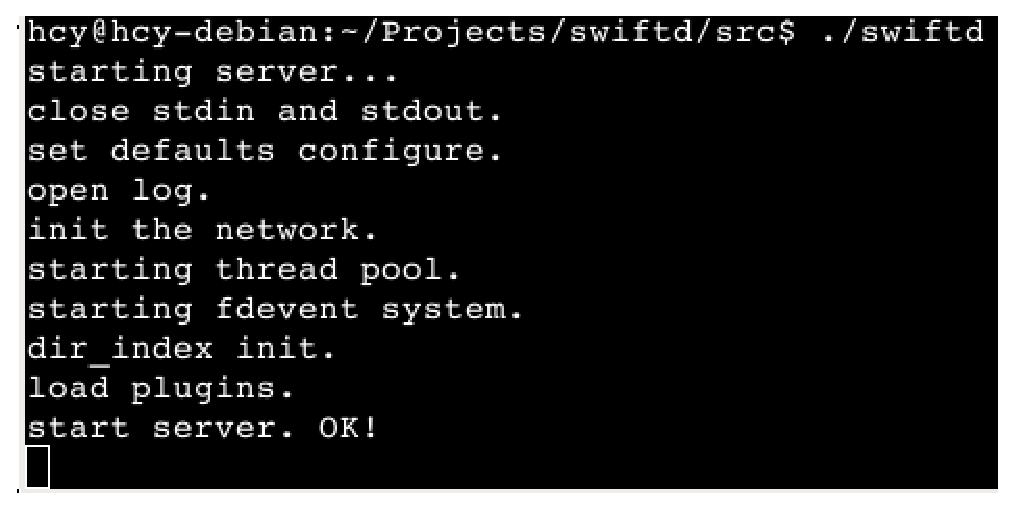
\includegraphics[height=6cm, width=15cm]{pics/startup.eps}
	\caption{服务器启动}
	\label{startup}
	\end{figure}
	
	在启动的控制台输出中可以看出服务器正常启动。
	
	启动日志。如图\ref{startuplog}。启动日志详细的记录了服务器的启动信息。
	\begin{figure}[htbp]
	\centering
	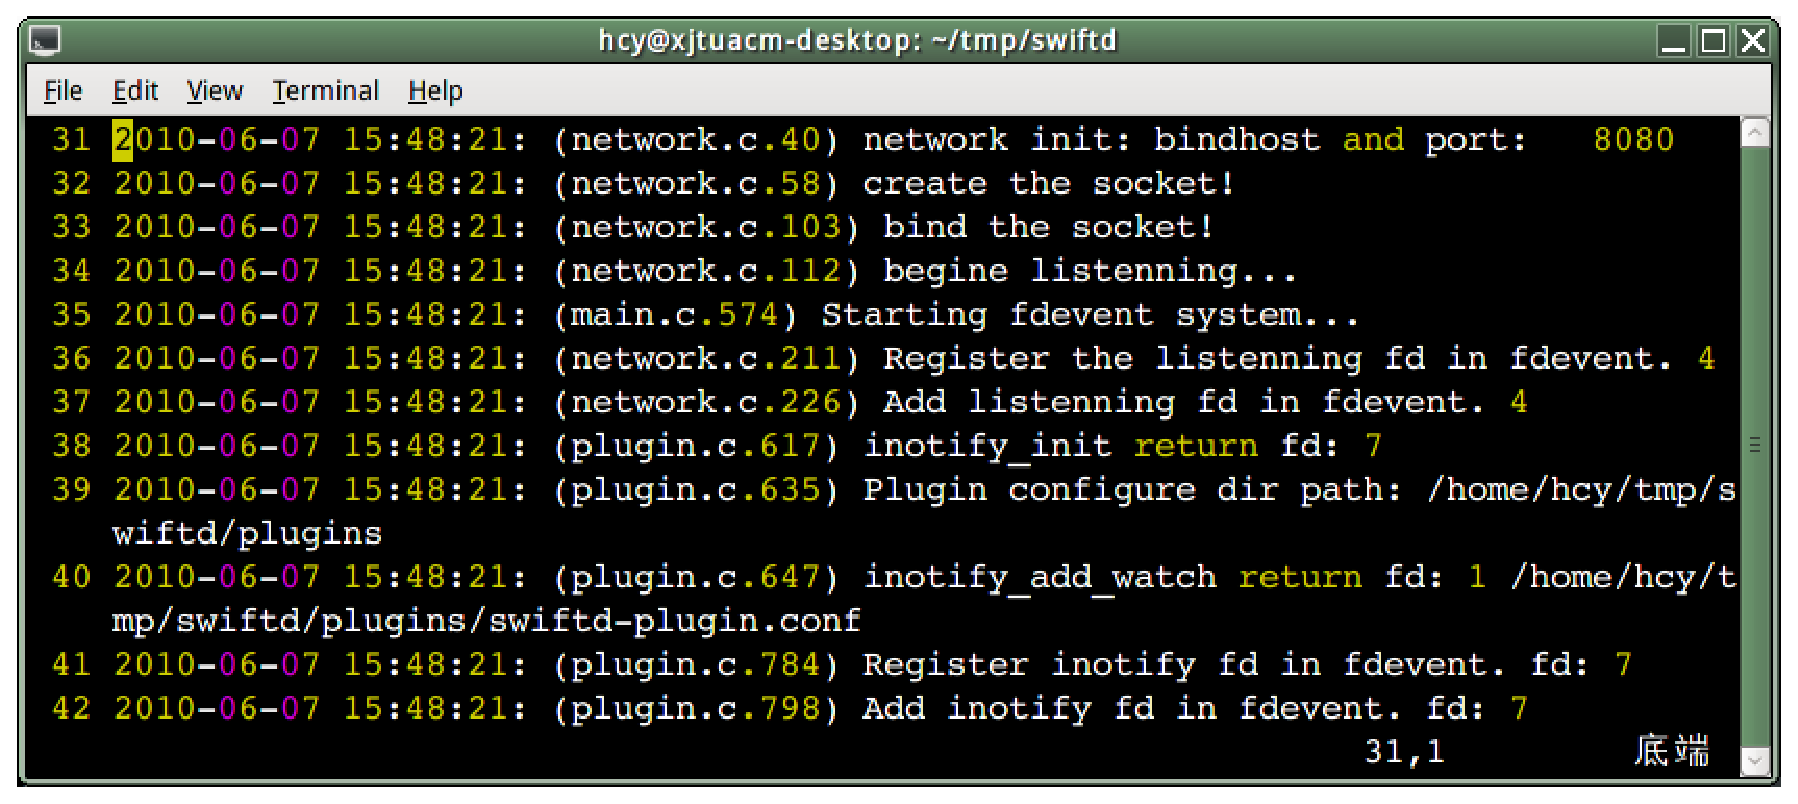
\includegraphics[height=7cm, width=16cm]{pics/startuplog.eps}
	\caption{启动日志}
	\label{startuplog}
	\end{figure}
	
	在服务器日志中同样显示服务器正常启动。监听8080端口。线程池,I/O多路复用系统都正常初始化。服务器通过Inotify开始对配置文件进行检测。服务器开始等待客户端请求。此时,服务器中没有任何插件。服务器只提供简单的返回静态资源的服务。
	
	通过浏览器访问服务器资源。如图\ref{access1}。图中浏览器地址栏中的地址必须有index.html,此时服务器还没有加载插件。如果访问目录的话,会返回404(资源不存在)错误。服务器对于定位到目录的资源请求,默认返回404错误。
	
	\begin{figure}[htbp]
	\centering
	\includegraphics[height=9cm, width=12cm]{pics/access1.eps}
	\caption{浏览器请求数据}
	\label{access1}
	\end{figure}
	
	浏览器得到了服务器返回的资源,服务器正确的处理的来自浏览器的请求。
	
	服务器请求处理日志。如图\ref{access1log}
	
	\begin{figure}[htbp]
	\centering
	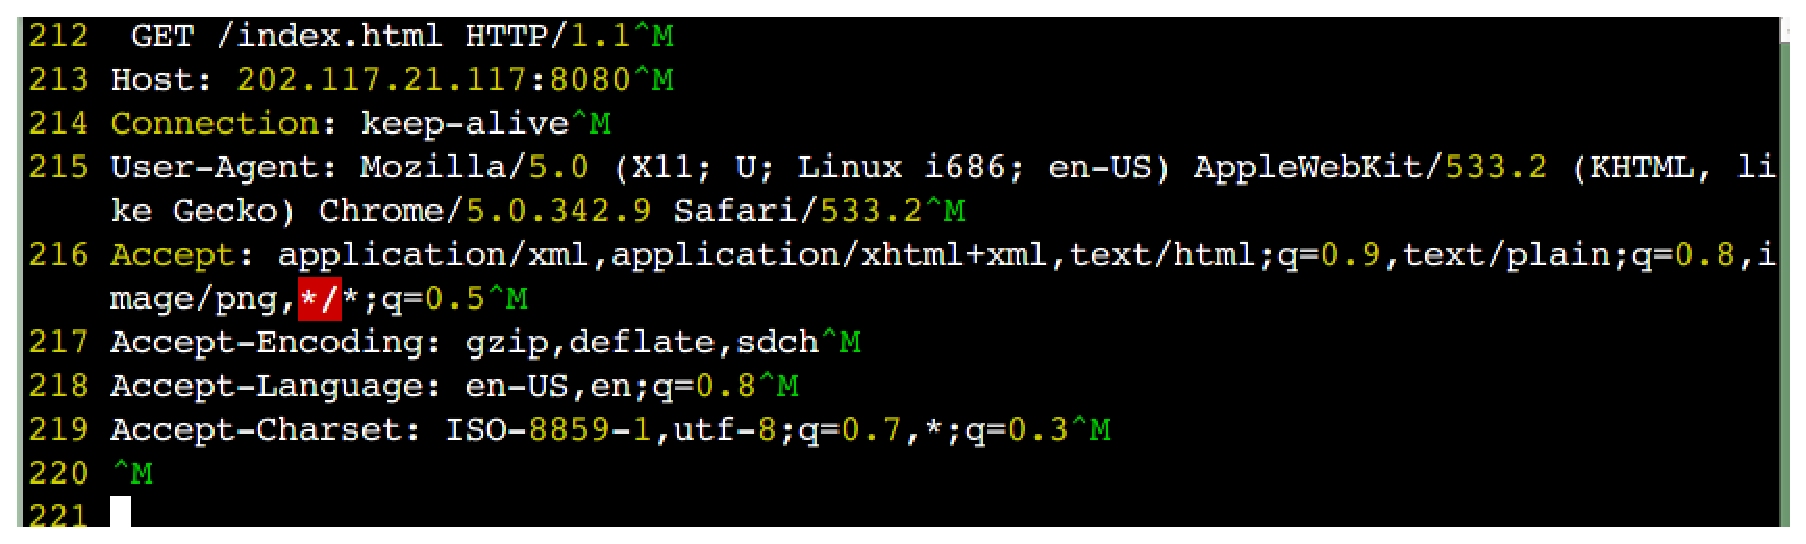
\includegraphics[height=5cm, width=15cm]{pics/access1log.eps}
	\caption{请求处理日志}
	\label{access1log}
	\end{figure}
	
	服务器的日志文件显示了本次请求的一些信息,主要包括HTTP请求头的数据。通过这些日志信息可以清除的看到服务器对各个请求的处理。日志中没有记录连接的次数,仅仅记录了各个请求的处理情况。
	
	
	加载插件。修改插件配置文件swiftd-plugin.conf。将插件的位置和名称写入配置文件中。保存。如图\ref{pluginconf}
	\begin{figure}[htbp]
	\centering
	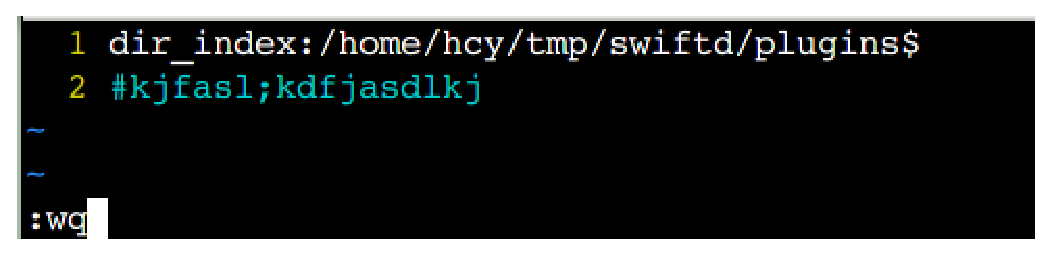
\includegraphics[height=3cm, width=10cm]{pics/pluginconf.eps}
	\caption{加载插件}
	\label{pluginconf}
	\end{figure}
	
	加载插件的日志。如图\ref{loadpluginlog}。从日志中我们可一看到,服务器检测到了配置文件的修改。接着,服务器重新读取了配置文件,然后加载插件。日志中还显示了插件所实现的结构。可以看到,插件实现了三个接口,服务器获得了所实现接口函数的入口地址。
	
	\begin{figure}[htbp]
	\centering
	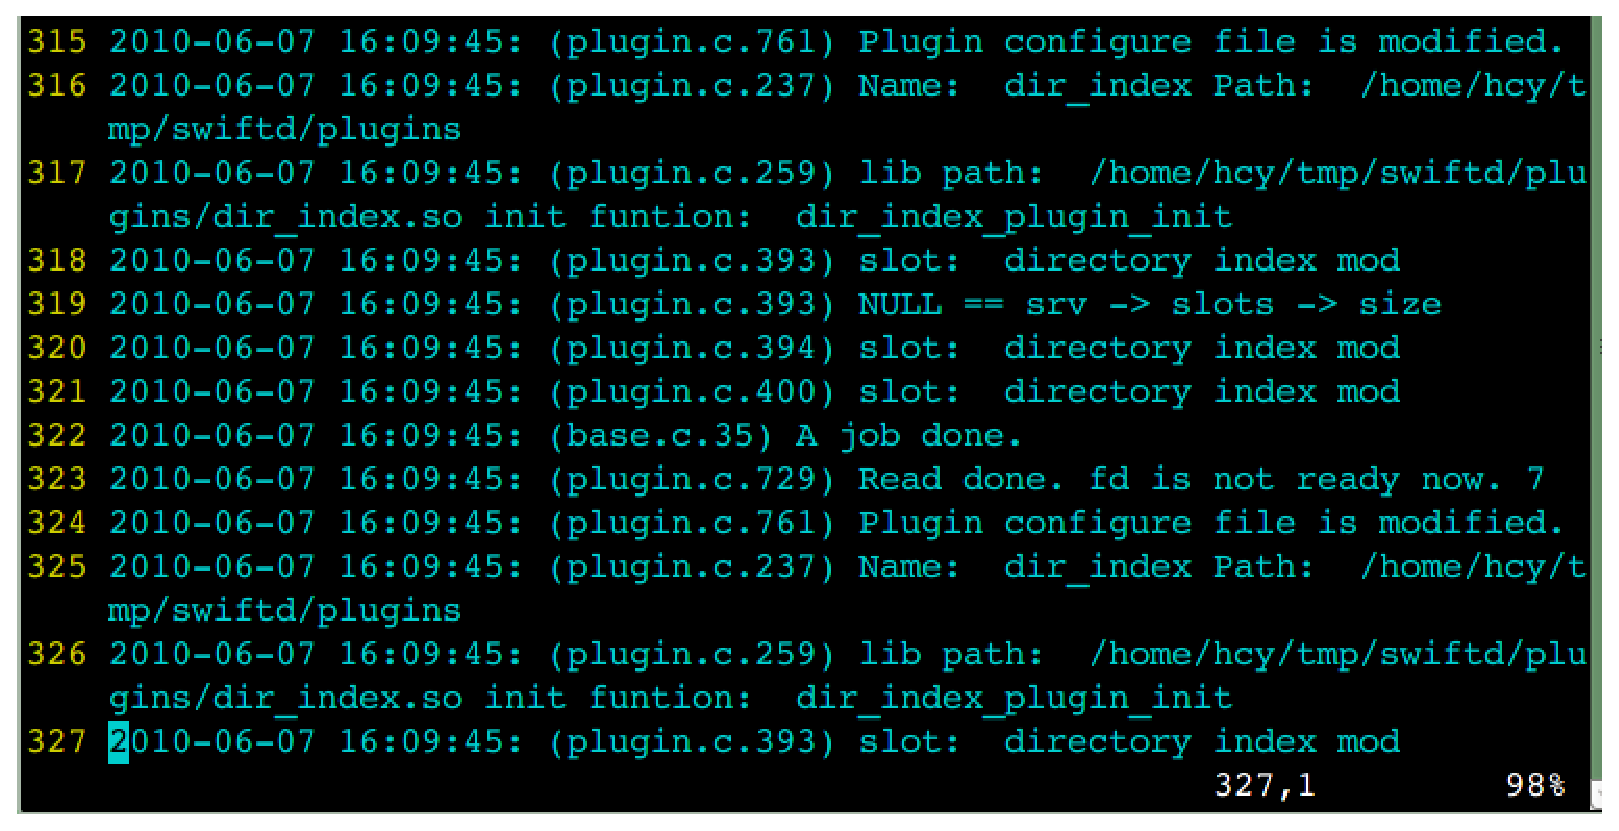
\includegraphics[height=9cm, width=15cm]{pics/loadpluginlog.eps}
	\caption{加载插件日志}
	\label{loadpluginlog}
	\end{figure}
	

	再次通过浏览器访问资源所在的目录。如图\ref{access2}。这个时候,服务器通过调用插件,完成在目录中搜索index.html的任务。如果搜索到这个文件,则返回这个文件。图\ref{access2}中显示服务器返回了目录下的index.html文件。
	\begin{figure}[htbp]
	\centering
	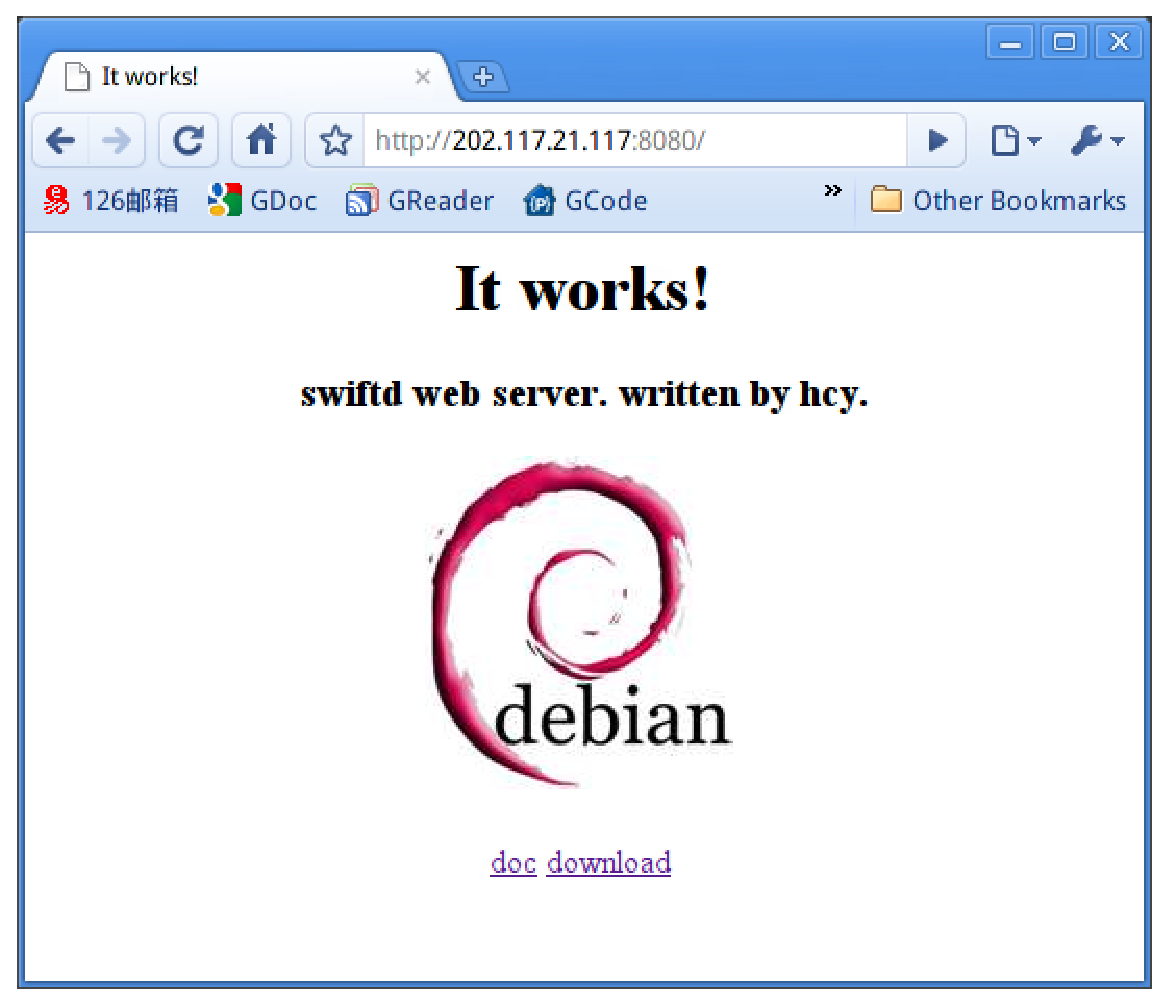
\includegraphics[height=9cm, width=12cm]{pics/access2.eps}
	\caption{浏览器请求数据,仅定位到目录}
	\label{access2}
	\end{figure}
	
	将插件卸载,删掉配置文件中的配置项。此时,服务器再次重新读取配置文件,删除配置文件中没有描述的插件。使用浏览器再访问资源所在目录。此时服务器返回404错误。

	
	测试结果总结如表\ref{testingresult}
	\begin{table}[htbp]
	\caption{测试结果:}
	\label{testingresult}
	\centering
	\begin{tabularx}{\textwidth}{p{1cm}XXXXl} %最后一列是空的。这样可以是倒数第二列居中,否则会报错或不居中。
	\toprule
	\centering 序号 & \centering  测试内容 & \centering  测试结果 &\centering 实际运行结果&\centering 是否符合要求&\\
	\midrule
	\centering 1 &\centering 启动并监听端口 &\centering 成功启动和监听端口 &\centering 成功启动和监听端口 & \centering 符合&\\
	\centering 2 &\centering 处理客户端请求 &\centering 返回请求资源 &\centering   返回请求资源& \centering 符合&\\
	\centering 3 &\centering 动态加载插件 &\centering  加载成功 &\centering  加载成功& \centering 符合&\\
	\centering 4 &\centering 调用插件 & \centering 正确调用插件 & \centering 正确调用插件& \centering 符合&\\
	\centering 5 &\centering 卸载插件 &\centering  卸载成功 &\centering  卸载成功& \centering 符合&\\
	\bottomrule
	\end{tabularx}
	\end{table}

%\subsection{性能测试}
%	处理大量请求。
	
%	传送大文件。
	
\section{本章小结}

	在本章中,论述了动态加载插件功能接口的实现,以及服务器的核心部分的实现,包括I/O,线程池和连接处理状态机,最后对服务器进行了测试。
	
	在动态加载插件功能接口的实现中,首先通过C语言的结构体和回调函数,实现功能接口的定义和调用。并且,使用面向对象的技术,实现解偶合。接着,利用Linux平台上的Inotify和动态链接技术,实现动态的检测和加载功能插件。最后,论述了如何实现一个功能插件。
	
	在服务器的实现中,重点论述了I/O,线程池和连接处理状态机的实现。服务器的I/O通过Linux下的epoll实现多路复用,线程池则借助Phtread库实现。连接处理状态机通过switch语句进行实现。
	
	在最后的测试中,服务器能够正确的动态的加载和卸载功能插件,并能够对功能插件的实现函数进行正确的调用嗯。服务器正确的处理了HTTP请求,并返回正确的处理结果。因此,服务器达到了课题目标的要求。
	
\chapter{结论与展望}
\section{结论}
	在三个月的毕业设计期间,本人查阅了大量HTTP协议的相关文献资料,重点分析了RFC2616,理解了HTTP协议处理的基本过程,包括请求的分析处理,回复的生成发送等。本人还搜集查阅了动态链接技术的相关资料,理解并掌握了动态链接技术的特点和使用。在此基础之上,通过分析HTTP协议的处理过程和动态链接技术,设计动态加载功能的接口。最后,通过实现一个服务器原型,完成接口的实现和验证。在此期间,本人学习了在Linux下进行C编程的知识,比如,使用gdb进行程序的调试,pthread库的使用,以及非阻塞I/O的使用等。通过这些知识的学习,使我系统的掌握了在linux下进行C开发的过程,也对Linux下的一些系统调用和库有了初步的了解。通过对HTTP协议的分析,本人了解了HTTP协议的处理过程,并且,通过实现web服务器的原型,是我对web服务器的设计有了初步的认识。在本论文中,首先阐述了课题的背景和意义,以及章节安排作者任务。然后,概述了一些有课题相关的技术。最后,详细的描述了系统的设计和实现,以及最后的运行测试结果。
	
	在毕业设计期间,本人完成的主要工作有:
	\begin{enumerate}
		\item 搜集学习有关动态链接技术和服务器设计技术的资料文献。掌握了动态链接技术的特点和应用,理解了HTTP协议的处理过程和主要的数据结构。
		\item 学习在Linux下进行服务器设计实现的相关技术。熟悉了gcc,gdb等工具的使用,对linux下的系统调用和库的使用有了初步的了解。
		\item 分析和设计动态加载功能的接口。通过分析HTTP协议的处理流程,设计接口和接口的调用过程。通过动态链接技术,设计动态加载功能的过程和方法。
		\item 在linux下对接口进行实现。通过实现一个web服务器的原型,在这个原型之上实现和验证所设计的接口。总共完成c代码约11000行。服务器可以完成功能的动态加载,能够正确的调用接口函数完成处理。服务器能够正确的处理HTTP请求。
		\item 对接口的实现进行测试和分析,确保实现的接口达到了预期的目的。
		\item 整理测试分析结果。完成毕业设计论文以及外文翻译。
	\end{enumerate}
	
\section{展望}
	随着互联网的高速发展,人们的生活越来越离不开互联网。越来越多的服务被从终端计算机搬到了互联网上。Google公司将要推出的网络操作系统chromeOS预示着未来的互联网将包含现在桌面PC的一切。随着应用规模的不断扩大,单一的服务器已经无法满足应用的需求。因此,分布式将成为互联网的未来。由于HTTP协议的先天特点,在分布式系统的应用中有着其得天独厚的优势。而HTTP协议的实现者————Web服务器必将是这些应用的中流砥柱。通过动态加载功能,web服务器将满足未来互联网应用的需求。随着硬件和操作系统能力的不断提高,web服务器将越来越强大。
	
	本系统没有对分布式系统进行考虑,不能很好的支持分布式应用。但是,在未来的互联网中,分布式将是主流。所有的服务器都会很好的支持分布式系统。

\five
\begin{thebibliography}{99}
\bibitem{cxyzwxy}俞甲子,石凡,藩爱民\quad 程序员的自我休养--链接、装载和库[M]\quad 电子工业出版社\quad 2009年4月
\bibitem{apue}W.Richard Stevens,Stepphen A. Rago 著\quad 尤晋元,张亚英,戚正伟 译\quad UNIX环境高级编程[M]\quad 第二版\quad 人民邮电出版社\quad 2008年12月
\bibitem{unp}W.Richard Stevens,Bill Fenner, Andrew M.Rudoff\quad UNIX Network Programming Volume 1:The Socket Networking API, Thrid Edition[M]\quad 人民邮电出版社\quad 2009年11月
\bibitem{usp}Kay A.Robbins, Steven Robbins 著\quad 陈涓,赵振平 译\quad UNIX系统编程[M]\quad 机械工业出版社\quad 2005年5月
\bibitem{pwpthread}David R. Butenhof\quad Programming with POSIX Threads[M]\quad Addison-Wesley\quad 2005年6月
\bibitem{sun}Sun Microsystems Inc.\quad 多线程编程指南[R]\quad 文件号码819–7051–10\quad 2006年10月
\bibitem{pp}Bil Lewis Daniel,J. Berg\quad PThreads Primer, A Guide to Multithreaded Programming[M]\quad SunSoft Press 2002年2月
\bibitem{http}R. Fielding,UC Irvine,J. Gettys等\quad Hypertext Transfer Protocol -- HTTP/1.1(RFC2616)[S]\quad Network Working Group\quad 1999年6月
\bibitem{WCW}Arlitt, T. Jin\quad Workload Characterization of the 1998 World Cup Web Site[M]\quad 1999年2月\quad http://www.hpl.hp.com/techreports/1999/HPL-1999-35R1.html.

\bibitem{wsw}F. Arlitt, C. L. Williamson\quad Web Server Workload Characterization: The Search for Invariants[M]\quad ACM SIGMETRICS Performance Evaluation Review\quad 24(1):126–137\quad 1996年5月

\bibitem{pp}Jon Bentley 著\quad 黄倩,钱丽艳 译\quad 编程珠玑[M]\quad 第二版本\quad 人民邮电出版社\quad 2008年10月
\bibitem{lighttpd}Lighttpd 1.4.20 源代码[CP]
\end{thebibliography}

%后面的chapter不需要标号。
\titleformat{\chapter}{\center \three \bf}{}{1em}{}

\lfour
\chapter{附录一: The C10k Problem}

It's time for web servers to handle ten thousand clients simultaneously, don't you think? After all, the web is a big place now.

And computers are big, too. You can buy a 1000MHz machine with 2 gigabytes of RAM and an 1000Mbit/sec Ethernet card for \$1200 or so. Let's see - at 20000 clients, that's 50KHz, 100Kbytes, and 50Kbits/sec per client. It shouldn't take any more horsepower than that to take four kilobytes from the disk and send them to the network once a second for each of twenty thousand clients. (That works out to \$0.08 per client, by the way. Those \$100/client licensing fees some operating systems charge are starting to look a little heavy!) So hardware is no longer the bottleneck.

In 1999 one of the busiest ftp sites, cdrom.com, actually handled 10000 clients simultaneously through a Gigabit Ethernet pipe. As of 2001, that same speed is now being offered by several ISPs, who expect it to become increasingly popular with large business customers.

And the thin client model of computing appears to be coming back in style -- this time with the server out on the Internet, serving thousands of clients.

With that in mind, here are a few notes on how to configure operating systems and write code to support thousands of clients. The discussion centers around Unix-like operating systems, as that's my personal area of interest, but Windows is also covered a bit.

\section*{I/O frameworks}

Prepackaged libraries are available that abstract some of the techniques presented below, insulating your code from the operating system and making it more portable.
	
	\begin{enumerate}
	
	\item ACE, a heavyweight C++ I/O framework, contains object-oriented implementations of some of these I/O 		
	strategies and many other useful things. In particular, his Reactor is an OO way of doing nonblocking I/O, and 
	Proactor is an OO way of doing asynchronous I/O.
	
	\item ASIO is an C++ I/O framework which is becoming part of the Boost library. It's like ACE updated for the STL era.
	\item libevent is a lightweight C I/O framework by Niels Provos. It supports kqueue and select, and soon will 
	support poll and epoll. It's level-triggered only, I think, which has both good and bad sides. Niels has a nice 
	graph of time to handle one event as a function of the number of connections. It shows kqueue and sys\_epoll as 
	clear winners.
	\item My own attempts at lightweight frameworks (sadly, not kept up to date):
		
		\begin{enumerate}
		\item Poller is a lightweight C++ I/O framework that implements a level-triggered readiness API using 
		whatever underlying readiness API you want (poll, select, /dev/poll, kqueue, or sigio). It's useful for 
		benchmarks that compare the performance of the various APIs. This document links to Poller subclasses below 
		to illustrate how each of the readiness APIs can be used.
		\item rn is a lightweight C I/O framework that was my second try after Poller. It's lgpl (so it's easier to 
		use in commercial apps) and C (so it's easier to use in non-C++ apps). It was used in some commercial 
		products.
		\end{enumerate}
		
	\item Matt Welsh wrote a paper in April 2000 about how to balance the use of worker thread and event-driven 
	techniques when building scalable servers. The paper describes part of his Sandstorm I/O framework.
	\item Cory Nelson's Scale! library - an async socket, file, and pipe I/O library for Windows
	
	\end{enumerate}

\section*{I/O Strategies}

Designers of networking software have many options. Here are a few:

	\begin{enumerate}
	\item Whether and how to issue multiple I/O calls from a single thread
		\begin{enumerate}
		\item Don't; use blocking/synchronous calls throughout, and possibly use multiple \\threads or processes to 
		    achieve concurrency
		\item Use nonblocking calls (e.g. write() on a socket set to O\_NONBLOCK) to start I/O, and readiness 
		    notification (e.g. poll() or /dev/poll) to know when it's OK to start the next I/O on that channel. 
		    Generally only usable with network I/O, not disk I/O.
		\item Use asynchronous calls (e.g. aio\_write()) to start I/O, and completion notification (e.g. signals or 
			completion ports) to know when the I/O finishes. Good for both network and disk I/O.
		
		\end{enumerate}
	\item How to control the code servicing each client
		\begin{enumerate}
		\item one process for each client (classic Unix approach, used since 1980 or so)
		\item one OS-level thread handles many clients; each client is controlled by:
			
			\begin{itemize}
			\item a user-level thread (e.g. GNU state threads, classic Java with green \\threads)
			\item a state machine (a bit esoteric, but popular in some circles; my favorite)
			\item a continuation (a bit esoteric, but popular in some circles)
			\end{itemize}
		\item one OS-level thread for each client (e.g. classic Java with native threads)
		\item one OS-level thread for each active client (e.g. Tomcat with apache front end; NT completion ports; 
			thread pools)
		\end{enumerate}
	\item Whether to use standard O/S services, or put some code into the kernel (e.g. in a custom driver, kernel 
		module, or VxD)
	\end{enumerate}
	
The following five combinations seem to be popular:

	\begin{itemize}
	\item Serve many clients with each thread, and use nonblocking I/O and level-triggered readiness notification
	\item Serve many clients with each thread, and use nonblocking I/O and readiness change notification
	\item Serve many clients with each server thread, and use asynchronous I/O
	\item serve one client with each server thread, and use blocking I/O
	\item Build the server code into the kernel
	\end{itemize}
\subsection*{Serve many clients with each thread, and use nonblocking I/O and level-triggered readiness notification}

... set nonblocking mode on all network handles, and use select() or poll() to tell which network handle has data waiting. This is the traditional favorite. With this scheme, the kernel tells you whether a file descriptor is ready, whether or not you've done anything with that file descriptor since the last time the kernel told you about it. (The name 'level triggered' comes from computer hardware design; it's the opposite of 'edge triggered'. Jonathon Lemon introduced the terms in his BSDCON 2000 paper on kqueue().)

Note: it's particularly important to remember that readiness notification from the kernel is only a hint; the file descriptor might not be ready anymore when you try to read from it. That's why it's important to use nonblocking mode when using readiness notification.

An important bottleneck in this method is that read() or sendfile() from disk blocks if the page is not in core at the moment; setting nonblocking mode on a disk file handle has no effect. Same thing goes for memory-mapped disk files. The first time a server needs disk I/O, its process blocks, all clients must wait, and that raw nonthreaded performance goes to waste. 

This is what asynchronous I/O is for, but on systems that lack AIO, worker threads or processes that do the disk I/O can also get around this bottleneck. One approach is to use memory-mapped files, and if mincore() indicates I/O is needed, ask a worker to do the I/O, and continue handling network traffic. Jef Poskanzer mentions that Pai, Druschel, and Zwaenepoel's 1999 Flash web server uses this trick; they gave a talk at Usenix '99 on it. It looks like mincore() is available in BSD-derived Unixes like FreeBSD and Solaris, but is not part of the Single Unix Specification. It's available as part of Linux as of kernel 2.3.51, thanks to Chuck Lever.

But in November 2003 on the freebsd-hackers list, Vivek Pei et al reported very good results using system-wide profiling of their Flash web server to attack bottlenecks. One bottleneck they found was mincore (guess that wasn't such a good idea after all) Another was the fact that sendfile blocks on disk access; they improved performance by introducing a modified sendfile() that return something like EWOULDBLOCK when the disk page it's fetching is not yet in core. (Not sure how you tell the user the page is now resident... seems to me what's really needed here is aio\_sendfile().) The end result of their optimizations is a SpecWeb99 score of about 800 on a 1GHZ/1GB FreeBSD box, which is better than anything on file at spec.org.

There are several ways for a single thread to tell which of a set of nonblocking sockets are ready for I/O:

	\begin{enumerate}
	\item The traditional select() 
	
	Unfortunately, select() is limited to FD\_SETSIZE handles. This limit is compiled in to the standard library and 
	
	user programs. (Some versions of the C library let you raise this limit at user app compile time.)
	
	See Poller\_select (cc, h) for an example of how to use select() interchangeably with other readiness 
	notification schemes.

	\item  The traditional poll()
	 
	There is no hardcoded limit to the number of file descriptors poll() can handle, but it does get slow about a 
	few thousand, since most of the file descriptors are idle at any one time, and scanning through thousands of 
	file descriptors takes time.
	
	Some OS's (e.g. Solaris 8) speed up poll() et al by use of techniques like poll hinting, which was implemented 
	and benchmarked by Niels Provos for Linux in 1999.

	See Poller\_poll (cc, h, benchmarks) for an example of how to use poll() interchangeably with other readiness 
	notification schemes.

	\item /dev/poll
	
	This is the recommended poll replacement for Solaris.
	
	The idea behind /dev/poll is to take advantage of the fact that often poll() is called many times with the same 
	arguments. With /dev/poll, you get an open handle to /dev/poll, and tell the OS just once what files you're 
	interested in by writing to that handle; from then on, you just read the set of currently ready file
	descriptors from that handle.

	It appeared quietly in Solaris 7 (see patchid 106541) but its first public appearance was in Solaris 8; 	
	according to Sun, at 750 clients, this has 10% of the overhead of poll().

	Various implementations of /dev/poll were tried on Linux, but none of them perform as well as epoll, and were 
	never really completed. /dev/poll use on Linux is not recommended.

	See Poller\_devpoll (cc, h benchmarks ) for an example of how to use /dev/poll interchangeably with many other 
	readiness notification schemes. (Caution - the example is for Linux /dev/poll, might not work right on Solaris.)

	\item kqueue()
	
	This is the recommended poll replacement for FreeBSD (and, soon, NetBSD).
	See below. kqueue() can specify either edge triggering or level triggering.
	
	\end{enumerate}
\subsection*{Serve many clients with each thread, and use nonblocking I/O and readiness change notification}

Readiness change notification (or edge-triggered readiness notification) means you give the kernel a file descriptor, and later, when that descriptor transitions from not ready to ready, the kernel notifies you somehow. It then assumes you know the file descriptor is ready, and will not send any more readiness notifications of that type for that file descriptor until you do something that causes the file descriptor to no longer be ready (e.g. until you receive the EWOULDBLOCK error on a send, recv, or accept call, or a send or recv transfers less than the requested number of bytes).

When you use readiness change notification, you must be prepared for spurious events, since one common implementation is to signal readiness whenever any packets are received, regardless of whether the file descriptor was already ready.

This is the opposite of "level-triggered" readiness notification. It's a bit less forgiving of programming mistakes, since if you miss just one event, the connection that event was for gets stuck forever. Nevertheless, I have found that edge-triggered readiness notification made programming nonblocking clients with OpenSSL easier, so it's worth trying.

[Banga, Mogul, Drusha '99] described this kind of scheme in 1999.

There are several APIs which let the application retrieve 'file descriptor became ready' notifications:
\begin{itemize}

	\item kqueue() This is the recommended edge-triggered poll replacement for FreeBSD (and, soon, NetBSD).
FreeBSD 4.3 and later, and NetBSD-current as of Oct 2002, support a generalized alternative to poll() called kqueue()/kevent(); it supports both edge-triggering and level-triggering. (See also Jonathan Lemon's page and his BSDCon 2000 paper on kqueue().)

Like /dev/poll, you allocate a listening object, but rather than opening the file /dev/poll, you call kqueue() to allocate one. To change the events you are listening for, or to get the list of current events, you call kevent() on the descriptor returned by kqueue(). It can listen not just for socket readiness, but also for plain file readiness, signals, and even for I/O completion.

Note: as of October 2000, the threading library on FreeBSD does not interact well with kqueue(); evidently, when kqueue() blocks, the entire process blocks, not just the calling thread.

See Poller\_kqueue (cc, h, benchmarks) for an example of how to use kqueue() interchangeably with many other readiness notification schemes.

Examples and libraries using kqueue():

\begin{itemize}
\item PyKQueue -- a Python binding for kqueue()
\item Ronald F. Guilmette's example echo server; see also his 28 Sept 2000 post on freebsd.questions.
\end{itemize}

\item epoll
This is the recommended edge-triggered poll replacement for the 2.6 Linux kernel.
On 11 July 2001, Davide Libenzi proposed an alternative to realtime signals; his patch provides what he now calls /dev/epoll www.xmailserver.org/linux-patches/nio-improve.html. This is just like the realtime signal readiness notification, but it coalesces redundant events, and has a more efficient scheme for bulk event retrieval.

Epoll was merged into the 2.5 kernel tree as of 2.5.46 after its interface was changed from a special file in /dev to a system call, sys\_epoll. A patch for the older version of epoll is available for the 2.4 kernel.

There was a lengthy debate about unifying epoll, aio, and other event sources on the linux-kernel mailing list around Halloween 2002. It may yet happen, but Davide is concentrating on firming up epoll in general first.

\item Polyakov's kevent (Linux 2.6+) News flash: On 9 Feb 2006, and again on 9 July 2006, Evgeniy Polyakov posted patches which seem to unify epoll and aio; his goal is to support network AIO. See:

\begin{itemize}
\item the LWN article about kevent
\item his July announcement
\item his kevent page
\item his naio page
\item some recent discussion
\end{itemize}

\item Drepper's New Network Interface (proposal for Linux 2.6+)
At OLS 2006, Ulrich Drepper proposed a new high-speed asynchronous networking API. See:

\begin{itemize}
\item his paper, "The Need for Asynchronous, Zero-Copy Network I/O"
\item his slides
\item LWN article from July 22
\end{itemize}

\item Realtime Signals
This is the recommended edge-triggered poll replacement for the 2.4 Linux kernel.
The 2.4 linux kernel can deliver socket readiness events via a particular realtime signal. Here's how to turn this behavior on:

\begin{verbatim}
/* Mask off SIGIO and the signal you want to use. */
sigemptyset(&sigset);
sigaddset(&sigset, signum);
sigaddset(&sigset, SIGIO);
sigprocmask(SIG_BLOCK, &m_sigset, NULL);
/* 
For each file descriptor, invoke F_SETOWN, F_SETSIG, and set O_ASYNC. 
*/
fcntl(fd, F_SETOWN, (int) getpid());
fcntl(fd, F_SETSIG, signum);
flags = fcntl(fd, F_GETFL);
flags |= O_NONBLOCK|O_ASYNC;
fcntl(fd, F_SETFL, flags);
\end{verbatim}

This sends that signal when a normal I/O function like read() or write() completes. To use this, write a normal poll() outer loop, and inside it, after you've handled all the fd's noticed by poll(), you loop calling sigwaitinfo().
If sigwaitinfo or sigtimedwait returns your realtime signal, siginfo.si\_fd and siginfo.si\_band give almost the same information as pollfd.fd and pollfd.revents would after a call to poll(), so you handle the i/o, and continue calling sigwaitinfo().

If sigwaitinfo returns a traditional SIGIO, the signal queue overflowed, so you flush the signal queue by temporarily changing the signal handler to SIG\_DFL, and break back to the outer poll() loop. 
See Poller\_sigio (cc, h) for an example of how to use rtsignals interchangeably with many other readiness notification schemes.

See Zach Brown's phhttpd for example code that uses this feature directly. (Or don't; phhttpd is a bit hard to figure out...)

[Provos, Lever, and Tweedie 2000] describes a recent benchmark of phhttpd using a variant of sigtimedwait(), sigtimedwait4(), that lets you retrieve multiple signals with one call. Interestingly, the chief benefit of sigtimedwait4() for them seemed to be it allowed the app to gauge system overload (so it could behave appropriately). (Note that poll() provides the same measure of system overload.)

\item Signal-per-fd
Chandra and Mosberger proposed a modification to the realtime signal approach called "signal-per-fd" which reduces or eliminates realtime signal queue overflow by coalescing redundant events. It doesn't outperform epoll, though. Their paper ( www.hpl.hp.com/techreports/2000/HPL-2000-174.html) compares performance of this scheme with select() and /dev/poll.

Vitaly Luban announced a patch implementing this scheme on 18 May 2001; his patch lives at www.luban.org/GPL/gpl.html. (Note: as of Sept 2001, there may still be stability problems with this patch under heavy load. dkftpbench at about 4500 users may be able to trigger an oops.)

See Poller\_sigfd (cc, h) for an example of how to use signal-per-fd interchangeably with many other readiness notification schemes.

\end{itemize}
\subsection*{Serve many clients with each server thread, and use asynchronous I/O}

This has not yet become popular in Unix, probably because few operating systems support asynchronous I/O, also possibly because it (like nonblocking I/O) requires rethinking your application. Under standard Unix, asynchronous I/O is provided by the aio\_ interface (scroll down from that link to "Asynchronous input and output"), which associates a signal and value with each I/O operation. Signals and their values are queued and delivered efficiently to the user process. This is from the POSIX 1003.1b realtime extensions, and is also in the Single Unix Specification, version 2.

AIO is normally used with edge-triggered completion notification, i.e. a signal is queued when the operation is complete. (It can also be used with level triggered completion notification by calling aio\_suspend(), though I suspect few people do this.)

glibc 2.1 and later provide a generic implementation written for standards compliance rather than performance.

Ben LaHaise's implementation for Linux AIO was merged into the main Linux kernel as of 2.5.32. It doesn't use kernel threads, and has a very efficient underlying api, but (as of 2.6.0-test2) doesn't yet support sockets. (There is also an AIO patch for the 2.4 kernels, but the 2.5/2.6 implementation is somewhat different.) More info:

\begin{itemize}
\item The page "Kernel Asynchronous I/O (AIO) Support for Linux" which tries to tie together all info about the 2.6 kernel's implementation of AIO (posted 16 Sept 2003)
\item Round 3: aio vs /dev/epoll by Benjamin C.R. LaHaise (presented at 2002 OLS)
\item Asynchronous I/O Suport in Linux 2.5, by Bhattacharya, Pratt, Pulaverty, and Morgan, IBM; presented at OLS '2003
\item Design Notes on Asynchronous I/O (aio) for Linux by Suparna Bhattacharya -- compares Ben's AIO with SGI's KAIO and a few other AIO projects
\item Linux AIO home page - Ben's preliminary patches, mailing list, etc.
\item linux-aio mailing list archives
\item libaio-oracle - library implementing standard Posix AIO on top of libaio. First mentioned by Joel Becker on 18 Apr 2003.
\end{itemize}

Suparna also suggests having a look at the the DAFS API's approach to AIO.

Red Hat AS and Suse SLES both provide a high-performance implementation on the 2.4 kernel; it is related to, but not completely identical to, the 2.6 kernel implementation.

In February 2006, a new attempt is being made to provide network AIO; see the note above about Evgeniy Polyakov's kevent-based AIO.

In 1999, SGI implemented high-speed AIO for Linux. As of version 1.1, it's said to work well with both disk I/O and sockets. It seems to use kernel threads. It is still useful for people who can't wait for Ben's AIO to support sockets.

The O'Reilly book POSIX.4: Programming for the Real World is said to include a good introduction to aio.

A tutorial for the earlier, nonstandard, aio implementation on Solaris is online at Sunsite. It's probably worth a look, but keep in mind you'll need to mentally convert "aioread" to "aio\_read", etc.

Note that AIO doesn't provide a way to open files without blocking for disk I/O; if you care about the sleep caused by opening a disk file, Linus suggests you should simply do the open() in a different thread rather than wishing for an aio\_open() system call.

Under Windows, asynchronous I/O is associated with the terms "Overlapped I/O" and IOCP or "I/O Completion Port". Microsoft's IOCP combines techniques from the prior art like asynchronous I/O (like aio\_write) and queued completion notification (like when using the aio\_sigevent field with aio\_write) with a new idea of holding back some requests to try to keep the number of running threads associated with a single IOCP constant. For more information, see Inside I/O Completion Ports by Mark Russinovich at sysinternals.com, Jeffrey Richter's book "Programming Server-Side Applications for Microsoft Windows 2000" (Amazon, MSPress), U.S. patent \#06223207, or MSDN.

\subsection*{Serve one client with each server thread}

... and let read() and write() block. Has the disadvantage of using a whole stack frame for each client, which costs memory. Many OS's also have trouble handling more than a few hundred threads. If each thread gets a 2MB stack (not an uncommon default value), you run out of *virtual memory* at (2\^30 / 2\^21) = 512 threads on a 32 bit machine with 1GB user-accessible VM (like, say, Linux as normally shipped on x86). You can work around this by giving each thread a smaller stack, but since most thread libraries don't allow growing thread stacks once created, doing this means designing your program to minimize stack use. You can also work around this by moving to a 64 bit processor.

The thread support in Linux, FreeBSD, and Solaris is improving, and 64 bit processors are just around the corner even for mainstream users. Perhaps in the not-too-distant future, those who prefer using one thread per client will be able to use that paradigm even for 10000 clients. Nevertheless, at the current time, if you actually want to support that many clients, you're probably better off using some other paradigm.

For an unabashedly pro-thread viewpoint, see Why Events Are A Bad Idea (for High-concurrency Servers) by von Behren, Condit, and Brewer, UCB, presented at HotOS IX. Anyone from the anti-thread camp care to point out a paper that rebuts this one? :-)

\subsubsection*{LinuxThreads}

LinuxTheads is the name for the standard Linux thread library. It is integrated into glibc since glibc2.0, and is mostly Posix-compliant, but with less than stellar performance and signal support.

\subsubsection*{NGPT: Next Generation Posix Threads for Linux}

NGPT is a project started by IBM to bring good Posix-compliant thread support to Linux. It's at stable version 2.2 now, and works well... but the NGPT team has announced that they are putting the NGPT codebase into support-only mode because they feel it's "the best way to support the community for the long term". The NGPT team will continue working to improve Linux thread support, but now focused on improving NPTL. (Kudos to the NGPT team for their good work and the graceful way they conceded to NPTL.)

\subsubsection*{NPTL: Native Posix Thread Library for Linux}

NPTL is a project by Ulrich Drepper (the benevolent dict\^H\^H\^H\^Hmaintainer of glibc) and Ingo Molnar to bring world-class Posix threading support to Linux.

As of 5 October 2003, NPTL is now merged into the glibc cvs tree as an add-on directory (just like linuxthreads), so it will almost certainly be released along with the next release of glibc.

The first major distribution to include an early snapshot of NPTL was Red Hat 9. (This was a bit inconvenient for some users, but somebody had to break the ice...)

NPTL links:

\begin{itemize}
\item Mailing list for NPTL discussion
\item NPTL source code
\item Initial announcement for NPTL
\item Original whitepaper describing the goals for NPTL
\item Revised whitepaper describing the final design of NPTL
\item Ingo Molnar's first benchmark showing it could handle 10\^6 threads
\item Ulrich's benchmark comparing performance of LinuxThreads, NPTL, and IBM's NGPT. It seems to show NPTL is much faster than NGPT.
\end{itemize}

Here's my try at describing the history of NPTL (see also Jerry Cooperstein's article):

In March 2002, Bill Abt of the NGPT team, the glibc maintainer Ulrich Drepper, and others met to figure out what to do about LinuxThreads. One idea that came out of the meeting was to improve mutex performance; Rusty Russell et al subsequently implemented fast userspace mutexes (futexes)), which are now used by both NGPT and NPTL. Most of the attendees figured NGPT should be merged into glibc.

Ulrich Drepper, though, didn't like NGPT, and figured he could do better. (For those who have ever tried to contribute a patch to glibc, this may not come as a big surprise :-) Over the next few months, Ulrich Drepper, Ingo Molnar, and others contributed glibc and kernel changes that make up something called the Native Posix Threads Library (NPTL). NPTL uses all the kernel enhancements designed for NGPT, and takes advantage of a few new ones. Ingo Molnar described the kernel enhancements as follows:

\begin{quotation}
While NPTL uses the three kernel features introduced by NGPT: getpid() returns PID, CLONE\_THREAD and futexes; NPTL also uses (and relies on) a much wider set of new kernel features, developed as part of this project.
Some of the items NGPT introduced into the kernel around 2.5.8 got modified, cleaned up and extended, such as thread group handling (CLONE\_THREAD). [the\\ CLONE\_THREAD changes which impacted NGPT's compatibility got synced with the NGPT folks, to make sure NGPT does not break in any unacceptable way.]

The kernel features developed for and used by NPTL are described in the design whitepaper, http://people.redhat.com/drepper/nptl-design.pdf ...

A short list: TLS support, various clone extensions (CLONE\_SETTLS, \\CLONE\_SETTID, CLONE\_CLEARTID), POSIX thread-signal handling, sys\_exit() extension (release TID futex upon VM-release), the sys\_exit\_group() system-call, sys\_execve() enhancements and support for detached threads.

There was also work put into extending the PID space - eg. procfs crashed due to 64K PID assumptions, max\_pid, and pid allocation scalability work. Plus a number of performance-only improvements were done as well.

In essence the new features are a no-compromises approach to 1:1 threading - the kernel now helps in everything where it can improve threading, and we precisely do the minimally necessary set of context switches and kernel calls for every basic threading primitive.
\end{quotation}

One big difference between the two is that NPTL is a 1:1 threading model, whereas NGPT is an M:N threading model (see below). In spite of this, Ulrich's initial benchmarks seem to show that NPTL is indeed much faster than NGPT. (The NGPT team is looking forward to seeing Ulrich's benchmark code to verify the result.)

\subsubsection*{FreeBSD threading support}

FreeBSD supports both LinuxThreads and a userspace threading library. Also, a M:N implementation called KSE was introduced in FreeBSD 5.0. For one overview, see \\www.unobvious.com/bsd/freebsd-threads.html.
On 25 Mar 2003, Jeff Roberson posted on freebsd-arch:

\begin{quotation}
... Thanks to the foundation provided by Julian, David Xu, Mini, Dan Eischen, and everyone else who has participated with KSE and libpthread development Mini and I have developed a 1:1 threading implementation. This code works in parallel with KSE and does not break it in any way. It actually helps bring M:N threading closer by testing out shared bits. ...
\end{quotation}

And in July 2006, Robert Watson proposed that the 1:1 threading implementation become the default in FreeBsd 7.x:

\begin{quotation}
I know this has been discussed in the past, but I figured with 7.x trundling forward, it was time to think about it again. In benchmarks for many common applications and scenarios, libthr demonstrates significantly better performance over libpthread... libthr is also implemented across a larger number of our platforms, and is already libpthread on several. The first recommendation we make to MySQL and other heavy thread users is "Switch to libthr", which is suggestive, also! ... So the strawman proposal is: make libthr the default threading library on 7.x.
\end{quotation}

\subsubsection*{NetBSD threading support}

According to a note from Noriyuki Soda:

\begin{quotation}
Kernel supported M:N thread library based on the Scheduler Activations model is merged into NetBSD-current on Jan 18 2003.
\end{quotation}

For details, see An Implementation of Scheduler Activations on the NetBSD Operating System by Nathan J. Williams, Wasabi Systems, Inc., presented at FREENIX '02.

\subsubsection*{Solaris threading support}

The thread support in Solaris is evolving... from Solaris 2 to Solaris 8, the default threading library used an M:N model, but Solaris 9 defaults to 1:1 model thread support. See Sun's multithreaded programming guide and Sun's note about Java and Solaris threading.

\subsubsection*{Java threading support in JDK 1.3.x and earlier}

As is well known, Java up to JDK1.3.x did not support any method of handling network connections other than one thread per client. Volanomark is a good microbenchmark which measures throughput in messsages per second at various numbers of simultaneous connections. As of May 2003, JDK 1.3 implementations from various vendors are in fact able to handle ten thousand simultaneous connections -- albeit with significant performance degradation. See Table 4 for an idea of which JVMs can handle 10000 connections, and how performance suffers as the number of connections increases.

\subsubsection*{Note: 1:1 threading vs. M:N threading}

There is a choice when implementing a threading library: you can either put all the threading support in the kernel (this is called the 1:1 threading model), or you can move a fair bit of it into userspace (this is called the M:N threading model). At one point, M:N was thought to be higher performance, but it's so complex that it's hard to get right, and most people are moving away from it.

\begin{itemize}
\item Why Ingo Molnar prefers 1:1 over M:N
\item Sun is moving to 1:1 threads
\item NGPT is an M:N threading library for Linux.
\item Although Ulrich Drepper planned to use M:N threads in the new glibc threading library, he has since switched to the 1:1 threading model.
\item MacOSX appears to use 1:1 threading.
\item FreeBSD and NetBSD appear to still believe in M:N threading... The lone holdouts? Looks like freebsd 7.0 might switch to 1:1 threading (see above), so perhaps M:N threading's believers have finally been proven wrong everywhere.
\end{itemize}

\subsection*{Build the server code into the kernel}

Novell and Microsoft are both said to have done this at various times, at least one NFS implementation does this, khttpd does this for Linux and static web pages, and "TUX" (Threaded linUX webserver) is a blindingly fast and flexible kernel-space HTTP server by Ingo Molnar for Linux. Ingo's September 1, 2000 announcement says an alpha version of TUX can be downloaded from ftp://ftp.redhat.com/pub/redhat/tux, and explains how to join a mailing list for more info. 

The linux-kernel list has been discussing the pros and cons of this approach, and the consensus seems to be instead of moving web servers into the kernel, the kernel should have the smallest possible hooks added to improve web server performance. That way, other kinds of servers can benefit. See e.g. Zach Brown's remarks about userland vs. kernel http servers. It appears that the 2.4 linux kernel provides sufficient power to user programs, as the X15 server runs about as fast as Tux, but doesn't use any kernel modifications.

\section*{Comments}

Richard Gooch has written a paper discussing I/O options.

In 2001, Tim Brecht and MMichal Ostrowski measured various strategies for simple select-based servers. Their data is worth a look.

In 2003, Tim Brecht posted source code for userver, a small web server put together from several servers written by Abhishek Chandra, David Mosberger, David Pariag, and Michal Ostrowski. It can use select(), poll(), epoll(), or sigio.

Back in March 1999, Dean Gaudet posted:

I keep getting asked "why don't you guys use a select/event based model like Zeus? It's clearly the fastest." ...

His reasons boiled down to "it's really hard, and the payoff isn't clear". Within a few months, though, it became clear that people were willing to work on it.

Mark Russinovich wrote an editorial and an article discussing I/O strategy issues in the 2.2 Linux kernel. Worth reading, even he seems misinformed on some points. In particular, he seems to think that Linux 2.2's asynchronous I/O (see F\_SETSIG above) doesn't notify the user process when data is ready, only when new connections arrive. This seems like a bizarre misunderstanding. See also comments on an earlier draft, Ingo Molnar's rebuttal of 30 April 1999, Russinovich's comments of 2 May 1999, a rebuttal from Alan Cox, and various posts to linux-kernel. I suspect he was trying to say that Linux doesn't support asynchronous disk I/O, which used to be true, but now that SGI has implemented KAIO, it's not so true anymore.

See these pages at sysinternals.com and MSDN for information on "completion ports", which he said were unique to NT; in a nutshell, win32's "overlapped I/O" turned out to be too low level to be convenient, and a "completion port" is a wrapper that provides a queue of completion events, plus scheduling magic that tries to keep the number of running threads constant by allowing more threads to pick up completion events if other threads that had picked up completion events from this port are sleeping (perhaps doing blocking I/O).

See also OS/400's support for I/O completion ports.

There was an interesting discussion on linux-kernel in September 1999 titled "> 15,000 Simultaneous Connections" (and the second week of the thread). Highlights:

\begin{itemize}
\item Ed Hall posted a few notes on his experiences; he's achieved >1000 connects/second on a UP P2/333 running Solaris. His code used a small pool of threads (1 or 2 per CPU) each managing a large number of clients using "an event-based model".
\item Mike Jagdis posted an analysis of poll/select overhead, and said "The current select/poll implementation can be improved significantly, especially in the blocking case, but the overhead will still increase with the number of descriptors because select/poll does not, and cannot, remember what descriptors are interesting. This would be easy to fix with a new API. Suggestions are welcome..."
\item Mike posted about his work on improving select() and poll().
\item Mike posted a bit about a possible API to replace poll()/select(): "How about a 'device like' API where you write 'pollfd like' structs, the 'device' listens for events and delivers 'pollfd like' structs representing them when you read it? ... "
\item Rogier Wolff suggested using "the API that the digital guys suggested", \\http://www.cs.rice.edu/\~gaurav/papers/usenix99.ps
\item Joerg Pommnitz pointed out that any new API along these lines should be able to wait for not just file descriptor events, but also signals and maybe SYSV-IPC. Our synchronization primitives should certainly be able to do what Win32's WaitForMultipleObjects can, at least.
\item Stephen Tweedie asserted that the combination of F\_SETSIG, queued realtime signals, and sigwaitinfo() was a superset of the API proposed in\\ http://www.cs.rice.edu/\~gaurav/papers/usenix99.ps. He also mentions that you keep the signal blocked at all times if you're interested in performance; instead of the signal being delivered asynchronously, the process grabs the next one from the queue with sigwaitinfo().
\item Jayson Nordwick compared completion ports with the F\_SETSIG synchronous event model, and concluded they're pretty similar.
\item Alan Cox noted that an older rev of SCT's SIGIO patch is included in 2.3.18ac.
\item Jordan Mendelson posted some example code showing how to use F\_SETSIG.
\item Stephen C. Tweedie continued the comparison of completion ports and F\_SETSIG, and noted: "With a signal dequeuing mechanism, your application is going to get signals destined for various library components if libraries are using the same mechanism," but the library can set up its own signal handler, so this shouldn't affect the program (much).
\item Doug Royer noted that he'd gotten 100,000 connections on Solaris 2.6 while he was working on the Sun calendar server. Others chimed in with estimates of how much RAM that would require on Linux, and what bottlenecks would be hit.
\end{itemize}
\chapter{附录二: c10k问题}
	现在的web服务器同时要处理上万个客户端,你不这样认为么?毕竟,现在互联网是一个强大的地方。
	
	计算机也同样强大。你可以花1200美元购买一台有1000MHz的CPU,2GB内存和1000Mbit/秒以太网卡的机器。让我们来看,有20000个客户端,每个客户端可以得到50Hz的CPU,100Kbytes的内存和50Kbits每秒的带宽。这不会消耗太多的时间为20000个客户端中的每一个客户端每一秒从磁盘读取4Kbytes的数据然后通过网络发送给她们。(顺便说一句,每个客户端花费0.08美元。一些操作系统费用中,每个客户端100美元的许可费用看起来有点重了!)因此,硬件已经不是瓶颈。
	
	1999年,一个最繁忙的ftp站点,cdrom.com,确实同时处理10000个客户端通过一个万兆以太网络。到了2001年,多个ISP服务商提供同样的速度,期望cdrom.com能够持续增长,以成为她们的大商业客户。
	
	这时,瘦客户端的计算模型似乎以某种形式回来了---在互联网上,服务器为成千上万的客户端同时提供服务。
	
	考虑到这一点,在如何配置操作系统和如何编写代码来支持成千上万的客户端,这里有一些札记。由于是我感兴趣的领域,这些讨论围绕类Unix操作系统,当然,Windows也会提及一点。	

\section*{I/O框架}
	目前有关于下面展示的技术的预先包装的库提供,这些库可以使你的代码不依赖于操作系统,使其更具可移植性。
	\begin{enumerate}
	
	\item ACE,一个重量级的C++ I/O框架,包含一些I/O策略的面向对象的实现和一些其他有用的东西。在具体实践中,他的Reactor模式是处理非阻塞I/O的一种面向对象处理方式,Proactor则是处理异步I/O的面向对象方式。
	\item ASIO是一个C++ I/O框架并且已经成为Boost库的一部分。它同ACE一样更新STL库。
	\item libevent是Niels Provos编写的一个轻量级的C I/O框架。它支持kqueue和select,并且很快就会支持poll和epoll。它仅有水平触发模式,我认为有好处也有坏处。Niels有一个不错的时间图处理一个作为连接数量的函数的事件。它显示kqueue和sys\_epoll是绝对的胜利者。
	\item 我自己的轻量级框架的尝试(很遗憾,没有持续更新):
		\begin{enumerate}
		\item Poller是一个轻量级的C++ I/O框架,实现了使用任何你想要的依赖就绪API(poll,select,/dev/poll,kqueue或者sigio)的水平触发就绪API。它对于比较不同API的表现的基准很有用处。下面这个连接到Poller子类的文档展示了如何使用每一个就绪API。
		\item rn是一个轻量级的C I/O框架,是我在Poller之后的第二次尝试。它是LGPL(因此更容易在社区程序中使用),用C编写(因此易于在非C++的程序中使用。)它在一些社区项目中被使用。
		\end{enumerate}
	\item Matt Welsh在2000年四月份写了一篇关于在构建可扩展服务器是平衡工作线程和事件驱动技术的使用的论文。论文中涉及了Sandstorm I/O框架的一部分。
	\item Cory Nelson's Scale!库--一个Windows上的非同步套接字,文件和管道的I/O库。
	\end{enumerate}
	
\section*{I/O策略}

网络软件设计人员有很多选择。下面就是一些:
	\begin{enumerate}
	
		\item 在一个单独的线程中是否处理多个I/O调用并且怎样处理。
		
			\begin{enumerate}
				\item 绝对。始终使用阻塞/同步调用,并且可能的话,使用多线程或多进程实现并发。
				\item 使用非阻塞调用(例如:write()一个套接字时设置为O\_NONBLOCK)来启动I/O,并且使用就绪通知机制(例如:poll()或者/dev/poll)来获得在那个通道上什么时候可以开始下一个I/O。
				\item 使用异步调用(例如:aio\_write())来开始I/O,并且使用完全通知机制(例如:信号或者完成端口)来获得I/O完成的时间。同时适用于网络和磁盘I/O。
			\end{enumerate}
		\item 怎样控制为每个客户端提供服务的代码。
			\begin{enumerate}
				\item 每个客户端一个进程(典型的Unix解决方案,从1980年开始使用)
				\item 一个操作系统层面的线程处理很多客户端。每个客户端的控制者为:
				\begin{enumerate}
					\item  一个用户层面的线程(例如:GNU状态线程,经典的Java绿色线程)
					\item  一个状态机(有点深奥,但是在一些地方很流行。我的最爱。)。
					\item  一个续集(有点深奥,但是同样在一些地方很流行)。
				\end{enumerate}
				\item 每个客户端一个操作系统层面的线程(例如:经典的Java本地线程)。
				\item 每个活动的客户端一个操作系统层面的线程(例如:Tomcat的\\apache前端,NT完成端口,线程池)。
			\end{enumerate}
		\item 是否使用标准的操作系统服务,或者把一些代码放到内核中。(例如:在一个第三方驱动,内核模块或者虚拟设备驱动(VxD))
	\end{enumerate}
	
	
下面的五种则和很流行:
	\begin{itemize}
		\item 一个线程处理多个客户端,使用非阻塞I/O和水平触发就绪通知机制。
		\item 一个线程处理多个客户端,使用非阻塞I/O和就绪状态改变通知机制。
		\item 多个线程处理多个客户端,使用异步I/O。
		\item 每个线程处理一个客户端,使用阻塞I/O。
		\item 把服务器代码加到内核中。
	\end{itemize}
	
\subsection*{一个线程处理多个客户端,使用非阻塞I/O和水平触发就绪通知机制。}

	将所有网络句柄设置成非阻塞模式,使用select()或者poll()来获知那个网络句柄有数据可读。这个是经典的传统模式。使用这种方案,操作系统内核告诉你那个文件描述符已经就绪,并且告诉你从最后一次内核告诉你这个事件是否你已经做了一些操作在那个文件描述符上。(名词“水平触发”来自计算机硬件设计。和“边际触发”相对。Jonathon Lemon在他的关于kqueue()的BSDCON 2000论文中介绍了这些。)
	
	注意:记住内核所发出的就绪通知仅仅是一个示意是很重要的。在你尝试从文件描述符读数据的时候,它可能压根就没有就绪。这就是为什么当使用就绪通知机制时使用非阻塞模式非常重要。
	这种方法的一个重要瓶颈是当请求的页此时不在核心上,read()或者sendfile()磁盘阻塞。将磁盘文件描述符设置成非阻塞没有什么作用。使用内存映射磁盘文件也一样。服务器第一次需要磁盘I/O时,它阻塞了,所有的客户端必须等待,这样原生非线程效率就被浪费了。
	
	这就是异步I/O要去解决的问题。但是在没有异步I/O的系统上,工作线程或进程进行磁盘I/O是依然会遇到这个瓶颈。一个解决方案是使用内存映射文件,如果mincore()标明需要I/O,调用一个工作线程去处理I/O,同时急促处理网络传输。Jef Poskanzer指出Pai, Druschel, 和Zwaenepoel的1999 Flash 网络服务器使用了这个方案。在Usenix '99他们有一个关于这个的讨论。似乎mincore()在一些BSD驱动的Unix,比如FreeBSD和Solaris上已经提供,但mincore()不是单一Unix标注的一部分。多亏Chuck Lever,mincore()作为Linux2.3.51内核的一部分提供。
	
	但是2003年11月在freebsd黑客列表中,Vivek Pei et al上报了一个不错的成果,他们利用系统剖析工具剖析它们的Flash Web服务器,然后再攻击其瓶颈。mincore是他们发现的其中之一的瓶颈(试想对所有情况那并不都是一个好办法)。另一个则是sendfile阻塞在磁盘访问上的事实。他们通过引进一个修改版的sendfile()来提高性能,这个修改版的sendfile()在当所需要获取的磁盘页不在核心上时,返回类似于EWOULDBLOCK的信息。(不能确定你如何告诉用户那个也现在在核心中了。。。在我看来,这里真正需要的是aio\_sendfile()。)他们优化的结果是在一个1GHz/1GB FreeBSD盒子中,获得了SpecWeb99的800分。这要优于spec.org上其他任何在文件上的方案。

对于一个单线程,有多种方法可以获知在一个非阻塞的套接字集合中,那个套接字已经有I/O就绪:

	\begin{enumerate}
	
	\item 传统的select().
	
	不幸的是,select()的FD\_SETSIZE有限制。这个限制被编译到标准库和用户程序中。(一些版本的C库可以让你在用户程序编译期间提高这个限制。)请查看Poller\_select(cc,h)关于如何使用select()和其他就绪通知方案互换的例子。
	
	\item 传统的poll()
	
	没有关于poll()所能处理的文件描述符的数量的硬编码的限制,但是由于在某一时间上,大多数的文件描述符处于等待状态并且扫描上千的文件描述符需要花费很多时间,当描述符的数量上千之后,它开始变慢。一些操作系统通过使用一些技术,比如轮询示意来提高poll()的速度。轮询示意在1999年被Niels Provos为Linux实现并成为标准。请查看Poller\_poll(cc,h)关于如何使用poll()和其他就绪通知方案互换的例子。
	
	\item /dev/poll
	
	这个是Solaris建议的poll的替代品。
	
	/dev/poll背后的思想是充分利用poll()经常被以相同的参数调用很多次的事实。通过/dev/poll,你得到一个打开的句柄。通过向这个句柄写数据,你只需要告诉操作系统一次你对什么文件感兴趣。之后,你只需要从那个句柄读一个当前就绪的文件描述符的集合。
	
	/dev/poll在Solaris7中悄然出现(查看106541补丁)。但是在Solaris8中才第一次公开出现。根据Sun的说法,在有750哥客户端时,/dev/poll比poll()有10%的效率提升。
	
	/dev/poll的不同实现都在Linux上试验过,但是没有一个性能可以epoll相当,并且没有一个实现真正完成。/dev/poll不建议在Linux上使用。
	
	请查看Poller\_devpoll(cc, h 基准)关于如何使用/dev/poll和其他就绪通知方案互换的例子。(注意:这个例子是在Linux的/dev/poll,可能在Solaris下不能正确工作)。
	\item kqueue()
	
	这个是FreeBSD建议的poll的替代品。(并且,也是NetBSD的)。下面指出,kqueue()可以设置成边际触发或者水平触发。
	
	\end{enumerate}
	
\subsection*{每一个线程处理多个客户端,使用非阻塞I/O和就绪通知机制。}

	就绪通知机制(或者边际触发就绪通知机制)表示你给内核一个文件描述符,之后,当这个描述符从没有就绪转换成就绪,内核在某个时候通知你。然后,操作系统内核就假设你已经知道那个文件描述符已经就绪。内核将不再发送那种类型的关于那个文件描述符的更多的就绪通知给你,直到你做了一些事情使文件描述符编程不就绪。(例如,直到你接受到一个EWOULDBLOCK错误在send,recv或者accept调用上,或者一次send或者recv传送的数据小于需要传送的字节数。)
	
	当你使用就绪改变通知机制时,你必须为假事件做好准备。因为一个通常的实现是当任何接受到数据包时就发送就绪信号,不管这个文件描述符是否就绪。
	
	这是“水平触发”就绪通知机制的对立面。由于你错过了仅仅一个事件,那么这个事件所对应的连接将永远处于等待状态,这是一个微小的编程错误疏忽。尽管如此,我发现边际触发就绪通知机制是使用OpenSSL的非阻塞客户端编程变得容易,因此,这值得去尝试。
	
	[Banga, Mogul, Drusha '99]在1999年描述了这种方案。
	
	有几种API可以是程序获得“文件描述符就绪”的通知:
	\begin{enumerate}
	
	\item kqueue()
	
	这是FreeBSD推荐的边际触发poll的替代品。(同样,很快也是NetBSD的)。
	
	FreeBSD4.3以及后续版本和NetBSD 2002年10月份的当前版本支持一个通用的poll()的候选者叫kqueue()/kevents()。支持边际触发和水平触发。(参见Jonathan Lemon's的主页和他的关于kqueue()的BSDCon 2000 论文。)
	
	和/dev/poll类似,你分配一个监听对象,但是不是通过打开文件/dev/poll,而是调用kqueue()去分配一个。为了改变你正在监听的事件,或者得到当前事件的列表,你在kqueue()返回的描述符上调用kevent()。它不仅可以监听套接字的就绪,还可以监听普通的文件描述符,信号,甚至I/O完成。
	
	注意:在2000年10月,FreeBSD的线程库不能很好的同kqueue()交互。显然,当 kqueue() 阻塞,整个进程阻塞,而不是调用的线程。
	
	参见Poller\_kqueue(cc, h,基准)关于如何使用kqueue()和其他就绪通知机制互换的例子。
	
	使用kqueue()的例子和库:
		\begin{enumerate}
			\item PyKQueue--一个Python的kqueue()包转。
			\item Ronald F. Guilmette的echo服务器的例子。参见他的2000年9月28日在\\freebsd.questions 上的帖子。
		\end{enumerate}
	\item epoll
	
	这是Linux 2.6内核推荐的边际触发poll的替代品。
	
	在2001年7月11日,Davide Libenzi建议了一个实时信号的候选者。他的补丁提供了他所谓的/dev/epoll\\www.xmailserver.org/linux-patches/nio-improve.html。这和实时信号就绪通知机制类似,但是他能合并冗余事件,并且有更高效的对付大批事件获得的机制。
	
	Epoll在他的接口从一个特殊的/dev中的文件改变成校内他调用,sys\_epoll之后,以2.5.46合并到2.5内核树中。另外有为2.4内核提供的旧版本的epoll的补丁。
	
	2002年在linux内核邮件列表中,围绕Halloween有一个关于同一epoll,aio和其他别的事件资源的长时间的讨论。讨论也许不会在发生,但是Davide一直努力坚定epoll为通常情况下的首选。

	\item Polyakov的kevent(Linux 2.6或更高版本)的新闻:在2006年2月9日和7月6日,Evgeniy Polyakov提交了他的补丁。这个补丁看上去像是epoll和异步io的统一。它的目标是支持网络异步IO。参见:
	\begin{itemize}
		\item 关于kevent的LWN报告
		\item 他的kevent主页
		\item 他的naio主页
		\item 一些最近的讨论。
	\end{itemize}
	
	\item Drepper的新网络接口(Linux2.6内核的方案)

		在2006年的OLS,Ulrich Drepper建议了一个新的高速异步网络API。参见:
	\begin{itemize}
		\item 他的论文。《异步零拷贝网络I/O的需求》
		\item 他的展示。
		\item 7月22日的LWN文稿。
	\end{itemize}

	\item 实时信号

		这个建议用来替换Linux2.4内核的边际触发poll。

		linux2.4内核可以通过一个特殊的实时信号传递套接字就绪事件。下面是怎样打开这个特性:

		\begin{verbatim}
/* 屏蔽SIGIO信号和你想使用的信号 */
sigemptyset(&sigset);
sigaddset(&sigset, signum);
sigaddset(&sigset, SIGIO);
sigprocmask(SIG_BLOCK, &m_sigset, NULL);

/* 对于每一个文件描述符,设置F_SETOWN,F_SETSIG和O_ASYNC. */
fcntl(fd, F_SETOWN, (int) getpid());
fcntl(fd, F_SETSIG, signum);
flags = fcntl(fd, F_GETFL);
flags |= O_NONBLOCK|O_ASYNC;
fcntl(fd, F_SETFL, flags);
		\end{verbatim}
		
		当一个普通的I/O函数,如read()或者write(),完成时,这个将发送一个信号。
为了使用这个特性,在外循环中写一个普通的poll()函数,在循环里面,在你处理完所有poll()函数监测到的有事件的描述符之后,你循环调用sigwaitinfo()函数。

		如果sigwaitinfo或者sigtimedwait给你返回了一个实时信号,那么 siginfo.si\_fd 和 siginfo.si\_band 和poll()被调用之后的pollfd.fd和pollfd.revents有着相同的信息。因此,你可以处理I/O事件,然后继续调用sigwaitinfo()。

		参见Poller\_sigio(cc, h)关于如何使用实时信号和其他就绪通知机制的互换。

		参见关于如何直接使用这个特性的Zach Brown的phhttpd的代码。

		[Provos, Lever和Tweedie 2000]描述了最近的phhttpd使用不同的sigtimedwait(),sigtimedwait4()的基准,使你可以在一个调用中获得多个信号。另外,sigtimedwait4()函数的一点好处似乎可以允许程序测量系统的负载(那么,程序就可以有合适的行为)。(注意,poll()提供了同样的测量系统负载的功能。)

	\item  每个描述符一个信号

		Chandra和Mosberger建议了一个名叫“Signal-per-fd”的对实时信号实现的修改。这个修改可以通过消除冗余事件来减少或者消除实时信号队列的溢出。但是,它没有epoll的效率高。他们的论文比较了这个结构和select以及/dev/poll的效率。

		Vitaly Luban在2001年5月18日宣布一个这个结构的补丁实现。他的补丁在\\www.luban.org/GPL/gpl.html。(住:在2001年9月,这个补丁在高负载的时候依然存在这稳定性问题。dkftpbench在大约4500个用户的时候可能触发一个oops,也就是正确的行为却输出了一个错误日志。)
		
		参见Poller\_sigfd(cc,h)关于如何使用signal-per-fd和其他就绪通知机制交互。
	\end{enumerate}
 
\subsection*{每个线程处理多个用户,使用异步I/O}
		
	可能由于很少的系统支持异步I/O,也可能是因为这需要(如同非阻塞I/O一样)你重新构思你的应用,异步I/O还没有在Unix系统上流行起来。在标准Unix上,异步I/O通过aio\_ 接口提供(看下面的“异步输入输出”的链接),这个接口将一个信号和信号值与每一个I/O操作关联。信号和他们的值被排队并高效的传递个用户进程。这个来自POSIX 1003.1b实时扩展和单一Unix标准的第二版。

	异步I/O通常和边际触发完成机制一起使用,例如,一个信号被存入队列中直到操作完成。(通过调用aio\_suspend(),异步I/O也可以和水平触发完成机制一起使用,但是我很少看到有人这么做。)

	glibc2.1以及后续版本提供了一个通用的实现,这个实现是为了遵守标准而不是效率。

	Ben LaHaise的Linux异步I/O实现被合并到linux内核主分支中,最为2.5.32版本。它不使用内核线程,并且有一个非常高效的底层api,但是(例如2.6.0-test2)还不支持套接字。(有关于2.4内核的补丁,但和2.5/2.6的实现有所不同。)更多信息:

	\begin{itemize}
		\item 页面“关于Linux的内核异步I/O支持”尝试去将所有的关于2.6内核中异步I/O实现的信息组织在一起。(2003年9月16日发布。)
		\item 第三论:异步I/O vs /dev/epoll。Benjamin C.R. LaHaise(在2002年的OLS上发表)
		\item Linux2.5内核支持的异步I/O,Bhattachary,Pratt,Pulaverty和Morgan著,IBM ; 在 2003年的OLS发表。
		\item Suparna Bhattachaya的Linux下的异步I/O设计手记。比较了Ben的异步 I/O 和 SGI 的KAIO以及一些其他的异步I/O项目。
		\item Linux异步I/O主页。
		\item linux-aio邮件列表
		\item libaio-oracle;在libaio之上实现了标准Posix异步I/O的库。在2003年9月18日被Joel Becker第一次提及。
	\end{itemize}

	Suparna还建议去看看DAFS的关于AIO的API的实现。

	Red Hat AS和Suse SLES都提供了一个在2.4内核上的高效的实现。它和2.6内核的实现有关系但不完全相似。

	在2006年2月,一个新的尝试提供网络异步I/O。参见上面的关于Evgeniy Polyakov的基于kevent的AIO。

	在1999年,SGI为Linux实现了一个高速的AIO。在1.1版本的时候,据说可以同时在磁盘I/O和套接字上很好的工作。它好像使用了内核线程。这对那些等不及Ben的AIO支持套接字的人们来说依然很有用。

	O'Reilly的书POSIX.4:真实世界的编程包括了一个很好的关于aio的介绍。

	Sun的网站上包含一个关于早期的非标准aio在Solaris上的实现的教程。值得一看。但是记住你要在"aioread"和"aio\_read"之间转换。

	注意,AIO没有提供一个在没有对z磁盘I/O阻塞情况下打开文件的途径。如果你关心关于打开磁盘文件时引起的睡眠,Linus建议你在不同的线程中调用open()函数,而不是希望一个aio\_open()系统调用。

	在Windows下,异步IO和“重叠I/O”,IOCP或者“IO完成端口”有联系。微软的IOCP将早先的艺术例如异步I/O(比如io\_write)和队列完成通知机制(如将\\aio\_sigevent 值和 aio\_write 一起使用)技术组合起来,并增加一个阻止一些请求以试图保持同一个单一的IOCP常量相关连的运行线程的数量的新想法。更多的信息参见Mark Russinovich在sysinternals.com上的文章《深入I/O完成端口》,Jeffrey Richter的书《编写Microsoft Windows 2000服务器端程序》, 美国专利号:\#06223207,或者MSDN。



\subsection*{每个客户端一个线程处理}
	
	...让read()和write()阻塞。由于有每一个客户端使用一个完整的栈框的缺点,这个方法浪费内存。很多操作系统在同时处理几百个线程是有一些麻烦。如果一个线程需要2MB的栈(这时通产的默认值),在运行了(2\^30 / 2\^21)512个线程时,你将耗尽一个32位机器的1GB用户可使用的虚拟内存(例如,x86上运行的linux)。你可以通过给每个线程分配更小的栈来克服这个问题,但是由于大多数线程库不允许在创建线程后增加线程栈,这样做意味着你要设计好自己的程序来减少栈的使用。你也可以通过移植到一个64位的机器来克服这个问题。

	Linux,FreeBSD和Solaris对线程的支持不断增强。同时64位处理器将很快称为主流用户的选择。也许在不久的将来,那些喜欢使用每个客户端一个线程的开发者将能够使用这个设计为10000个客户端提供服务。但是,就目前而言,如果你真的想支持那么多用户,你最好使用别的设计。

	对于一些支持线程的观点,参见Behren,Condit和Brewer的《为什么时间不是好东西(对于高并发服务器)》,UCB,在HotOs IX发表。有没有发对线程的人发表一篇文章来驳斥这个观点?

\subsubsection*{LinuxThreads}
	LinuxThreads是标准Linux线程库的名称。从glibc2.0开始,它被集成到glibc中。它几乎是Posix兼容的,但是缺少效率和信号支持。

\subsubsection*{NGPT:Linux下一代线程}
	NGPT是IBM发起的旨在为Linux提供一个好的Posix兼容的线程支持。它现在的稳定版本是2.2,并且运行的很好。。。但是NGPT开发团队已经宣布他们将NGPT的代码库设置为仅支持不开发的模式。因为他们感觉这是“最好的长时间支持社区的办法”。NGPT开发团队将继续改进Linux的线程支持,但是现在他们的重点是改进NPTL。(荣誉属于NGPT团队,为他们优秀的工作和他们考虑NPTL的优雅的方法。)

\subsubsection*{NPTL:Linux原生Posix线程库}
	NPTL是Ulrich Drepper(和蔼的glibc的维护者)和Ingo Molnar发起的项目,旨在为Linux带来世界级的Posix线程支持。

	在2003年10月5日,NPTL被合并到glibc的版本控制树中,最为一个附加的目录(就像linuxthreads一样),因此,它几乎确定将在gblic的下一个发布版中发布。

	Red Hat9是第一个包含NPTL早期快照的主流发行版。(这也许对一些用户不太方便,但是必须有人能够破冰。。。)

	NPTL的链接:
	\begin{itemize}
		\item NPTL讨论邮件列表
		\item NPTL源码
		\item NPTL的初始声明
		\item 描述NPTL最终设计的原始白皮书
		\item 描述NPTL最红设计的修订白皮书
		\item Ingo Molnar的第一个测试标准现实NPTL可以处理10\^6个线程
		\item Ulrich的比较LinuxThreads,NPTL和IBM的NGPT的测试基准。这个似乎显示 NPTL 比 NGPT快多了。
	\end{itemize}

	下面是我关于NPTL历史的一些描述(同时参见Jerry Cooperstein的文章):

	在2002年5月,NGPT的成员Bill Abt,glibc的维护者Ulrich Drepper和一些其他人见面讨论要对LinuxThreads做些什么。来自那次见面的一个想法是提高互斥锁的效率。 Rusty Russell et al后来实现了快速用户空间互斥锁(futexes),并且现在正被NGPT和NPTL使用。大部分的参与者认为NGPT应该合并到glibc中。

	然而Ulrich Drepper不喜欢NGPT,并且他指出他可以做的更好。(对那些曾经给\\glibc贡献过补丁的人来说,这也许不是什么吃惊的事。)在下面的几个月中,Ulrich Drepper,Ingo Molnar和其他一些人贡献了一些对glibc和内核的修改,被称作原生Posix线程库(NPTL)。NPTL使用了内核为NGPT设计的增强功能,并且利用了一些新的功能。Ingo Molnar如下的描述了这些内核增强功能:

	\begin{quotation}
		当NPTL使用了NGPT引入的三个内核特性:getpid()返回PID,\\ CLONE\_THREAD 和 futexes,NPTL也使用(并且依赖)了一些更宽泛的内核特性,这些特性作为这个项目的一部分。

		一些NGPT在2.5.8时引入的内核特性被修改,清除和扩展,例如线程组处理(CLONE\_THREAD)。(CLONE\_THREAD的修改影响了NGTP的和其他NGPT亲戚同步的兼容性,为了保证在任何不可接受的情况下NGPT都不会中断。)
		
		为NPTL设计并被NPTL使用而开发的内核特性在设计白皮书中描述。http://people.redhat.com/drepper/ntpl-design.pdf...

		一个简短列表:TLS支持,多种克隆扩展(CLONE\_SETLS, CLOSE\_SETTID, CLONE\_CLEARTID),POSIX线程信号处理, \\sys\_exit()扩展(在VM发布版上发布了TID futex),sys\_exit\_group()系统调用,sys\_execve()加强和分离线程的支持。

		还有关于扩展PID空间的工作被做,例如,由于64K PID的假设,max\_pid和pid分配扩展性工作,procfs会崩溃。还有一些仅性能方面的提高的工作也被做了。

		本质上,新的特性是实现1:1线程的非妥协处理。现在内核可以在任何提高线程能力的地方有所版主,并且我们只需要做上下文切换和基本线程原函数的内核调用的很小的一部分。
	\end{quotation}

	两者之间最大的却别在于NPTL是1:1的线程模型,而NGPT是M:N的线程模型(参见下面)。尽管如此,Ulrich的初始基准似乎显示NPTL确实毕NGPT快多了。(NGPT团队期待看打Ulrich的基准代码来修改结果。)

\subsubsection*{FreeBSd的线程支持}
	
	FreeBSD支持LinuxThreads和一个用户空间线程库。另外,一个叫做KSE的\\M:N的实现在FreeBSD5.0时被引入。参见www.unobvious.com/bsd/freebsd-threads.html

	在2003年5月25日,Jeff Roberson在freebsd-arch发了一个贴:
	\begin{quotation}
		...幸亏Julian, David Xu, Mini, DanEischen和所有其他投身KSE和libpthread\\开发的人建立的基础,Mini和我开发出了一个1:1的线程实现。这个实现和KSE并行运行宾切不会打断KSE。它实际上通过测试共享位,帮助我们更靠近了M:N线程模型。
	\end{quotation}

	在2006年7月,Robert Watson宣布在FreeBSD7.x中,1:1线程模型实现成为默认的:

	\begin{quotation}
		我知道这个在以前已经讨论过了,但是由于7.x的不断改进,我认为现在该再次考虑它了。在很多常规应用和情景的基准中,libthr显然毕libpthread有更好的性能...libthr实现了跨很多平台,并且包含那些libpthread已经支持的一些平台。第一个我们为MySQL和其他大量线程用户的建议是“改用libthr”,libthr也是推荐的!...因此strawman的建议是:是libthr成为7.x的默认线程库。
	\end{quotation}

\subsubsection*{NetBSD的线程支持}
		根据Noriyuki Soda的手记:
		
		在2003年7月18日,基于调度激活模型的支持M:N线程库的内核被合并到BetBSD当前版本中。

		更多细节参见Nathan J. Williams, Wasabi Systes, Inc.在FRENIX上发表的的\\NetBSD操作系统上调度激活的一个实现。
\subsubsection*{Solaris的线程支持}
	
	Solaris的线程支持在不断的演变。从Solaris2到Solaris8,默认的线程库是M:N模型,但是在Solaris9默认的线程库是1:1模型。参见Sun的多线程编程手册和Sun的关于Java和Solaris线程的手册。

\subsubsection*{在JDK1.3.x及后续版本中Java的线程支持}

	众所周知,Java直到JKD1.3.x都没有提供任何处理网络连接的方法,除了一个客户端一个线程。Volanomark是一个不错的微型测试程序,可以用来测量在某个时候不同数目的网络连接时每秒钟的信息吞吐量。在2003.5, JDK 1.3的实现实际上可以同时处理10000个连接,但是性能却严重下降了。从Table 4 可以看出JVMs可以处理10000个连接,但是随着连接数目的增长性能也逐步下降。

	注:1:1模型 vs M:N模型

	在实现线程的时候,你有一个选择:你可以把所有线程的支持都放入内核中(这被成为1:1模型)或者你可以把一部分的线程支持移到用户空间中(这被成为M:N模型)。有一个观点认为,M:N模型有更高的性能,但是它太过复杂以致很难保证正确,并且大多数人正在远离他。
	\begin{itemize}
		\item 为什么Ingo Molnar更喜欢1:1,而不是M:N
		\item Sun正在转移到1:1模型上。
		\item NGPT是一个Linux下的M:N模型线程库。
		\item 尽管Ulrich Drepper计划在新的glibc线程库中使用M:N模型,但是他曾经转移到1:1模型过。
		\item MaxOSX看来使用1:1模型。
		\item FreeBSd和NetBSD似乎依然坚守M:N模型...最长的坚守者?好像freebsd7.0也许转移到1:1线程模型(参见上文),所以也许M:N线程模型的坚守者被证明一无是处。
	\end{itemize}
\subsection*{将服务器代码嵌入内核}

	Novell和微软在不同的时间都宣称已经实现了这个。至少,一个NFS的实现是这样的,khttpd是linux下的静态网页服务器,"TUX"(Threaded linUX webserver)是Ingo Molnar为Linux实现的相当快并且可扩展的内核空间HTTP服务器。Ingo在2000年9月1日的声明说一个alpha版本的TUX可以在ftp://ftp.redhat.com/pub/redhat/tux上下载,并且说明怎样加入一个邮件列表以获得更多的信息。

	linux-kernel邮件列表已经一直在讨论这个实现的优缺点,讨论的共识似乎是内核应该提供最小的可能的hooks的增加以提高web服务器的性能,而不是将web服务器移到内核中。这种方法也可使其他服务器受益。参见Zach Brown的关于用户空间vs内核http服务器的备注。linux2.4内核提供了有效的功能给用户程序,比如X15服务器运行的和Tux一样快,但没有对内核进行任何修改。
	
\section*{注解}
	Richard Gooch写了一篇讨论I/O选项的论文。
	
	在2001年,Tim Brecht和MMichal Ostrowski测量了各种策略下的简单基于select服务器的性能。他们的数据值得一看。

	在2003年,Tim Brecht发布了userver的源代码。这是一个下的web服务器,集合了Abhishek Chandra,David Mosberger,David Pariag和Michal Ostrowski所写的多个服务器。它可以使用select(),poll(),epoll()或者sigio。

	回到1999年五月,Dean Gaudet发帖说:

	我不断地被问道“为什么你们这些人不使用基于select/event的模型,就像Zeus?很明显那是最快的。”...

	他的理由归结为“很困难,并且回报不明显”。但是几个月后,越来越明显,人们喜欢使用它。

	Mark Russinovich写了一篇社论和论文讨论关于Linux2.2内核的I/O策略。值得一读,虽然他似乎乎略了一些观点。实际上,他似乎认为Linux2.2内核的异步I/O(参见上文F\_SETSIG)不会在数据准备就绪时通知用户进程,而是仅仅在新连接到达时通知。这看起来是一个异乎寻常的误解。参见一个早期草案的注解,Ingo Molnar在1999年4月30日的反驳,Russinovich在1999年5月2日的注解,Alan Cox的反驳和linux-kernel的帖子。我猜测他试图在说Linux不支持异步磁盘I/O,这个曾经确实是对的。但是现在,SGI已经实现了KAIO,这个不在是对的了。

	参见这些关于“完成端口”的sysinternals.com和MSDN的网页。他认为完成端口是NT特有的。总之,win32的“覆盖I/O”过于底层而不方便使用,并且一个“完成端口”是一个包装,提供了完成事件的队列,外加通过当别的已经从这个端口获得完成事件的线程处于睡眠状态时(可能在做阻塞I/O), 允许更多更多的线程获得完成事件来保持运行状态的线程数量保持不变。
	
	参见OS/400的对完成端口的支持。

	1999年9月,在linux-kernel上有一个内部的讨论,“>15000并发连接”(线程的第二个星期)。主要包括:

	\begin{itemize}
		\item Ed Hall发布了一些关于他的经验的手记。他的在一个运行Solaris的HP P2/333上实现>1000 个连接/秒的方案。他的代码使用了一个小的线程池(1或2个每个CPU)每个线程处理大量客户端使用“一个基于事件的线程”。
		\item Mike Jagdis发布了一个关于poll/select开销的分析,他说“当前的select/poll实现可以被显著的提高,尤其是在阻塞的情况下。但是开销依然会随着描述符数量的增加而增加,这是因为select/poll没有,也不可能记住哪些描述符可能有事件。这个很容易通过一个新的API来修正。欢迎提建议...”
		\item Mike发布了他的关于提高select()和poll()性能的工作。
		\item Mike发布了一点关于一个可能替换select()/poll()的API:“在一写‘类pollfd’结构体的地方,一个‘类设备’的API如何,这个‘设备’监听事件并且在你读它的时候,它传送‘类pollfd’结构体来表示事件?...”
		\item Rogier Wolff建议使用“数字开发人员建议的API”,http://www.cs.rice.edu/\~gaurav/papers/usenix99.ps
		\item Joerg Pommnitz指出,这个讨论中的任何新的API必须不仅仅能构等待文件描述符的事件,还要能够等待信号和也许SYSV-IPC。至少,我们的同步原语能够确切的完成Win32的WaitForMultipleObjects能够完成的任务。
		\item Stephen Tweedie断言,F\_SETSIG,实时信号队列和sigwaitinfo()的组合是http://www.cs.rice.edu/\~gaurav/papers/usenix99.ps所提到的API的超集。他还提到,如果你很在意效率,那么一致保持信号阻塞。否则,进程从sigwaitinfo()的队列中抓取下一个信号,而不是异步的传送信号。
		\item Jayson Nordwick比较了完成端口和F\_SETSIG同步事件模型,得出的结论是他们非常的相似。
		\item Alax Cox指出,一个旧的SCT的SIGIO的rev补丁包含在2.3.18ac中。
		\item Jordan Mendelson发布了一些如何使用F\_SETSIG的示例代码。
		\item Stephen C. Tweedie继续比较了完成端口和F\_SETSIG,指出“当使用一个信号队列机制时,如果正在使用的库也使用了相同的机制,那么,你的程序将获得那些本来属于各种库组件的信号。”但是,库可以设置自己的信号处理函数,因此这个不会(过多)的影响程序。
		\item Doug Royer指出,当他在Sun日期服务器上工作的时候,他获得了100000个连接在Solaris2.6上。其他的关于如何估计在Linux需要多少RAM和将会遇到什么瓶颈的文章。
	\end{itemize}
	
\chapter{致谢}

本论文及系统的完成得益于许多人的帮助与支持,在此对所有帮助过我的老师与同学表示由衷的感谢!

首先感谢指导老师马瑞芳老师的辛勤指导,对本论文及系统提出了许多意见并给出了改进方案,指明了道路。她每周都能够在白忙之中抽出一早晨时间,来给我们做进度规划,帮助我们分析问题,解决问题,督促我们抓紧时间,这对于我们能够按照预订计划完成工作有很大的帮助,马老师孜孜不倦的工作精神以及耐心的工作态度是我们毕设组同学如期完成论文以及系统的重要保障,在此,我对马老师致以崇高的敬意以及衷心的感谢!

下面要感谢学院给我们提供了专门的机房机位,这极大的方便了我们进行毕业设计。尤其是机房的管理员老师,每当机房出现网络问题时,管理员老师总是第一时间赶来处理问题,为我们节省时间。再次,对管理员老师表示衷心的感谢。

还有就是要感谢BBS上帮我解决问题的那些同学们。虽然我不知道你们叫什么名字,那个学院,甚至你们是男生还是女生。但是,每当我遇到问题求助时,你们总是能够耐心的帮我解决问题。在毕设过程中,你们给予了我莫大的帮助,对你的无私帮助,我表示最衷心的感谢!

最后,衷心感谢在百忙之中抽出时间评阅本论文的专家教授们。
\end{document}
